%-------------------------------------------------------------------------------
%                            BAB IV
%               		HASIL DAN PEMBAHASAN
%-------------------------------------------------------------------------------
\fancyhf{} 
\fancyfoot[C]{\thepage}
\chapter{HASIL DAN PEMBAHASAN}

\section{\uppercase{Analisis Kebutuhan}}
Analisis kebutuhan merupakan tahapan yang dilakukan untuk mengetahui pengguna yang terlibat dalam aplikasi yang akan dibangun serta mengetahui kebutuhan-kebutuhan dari setiap pengguna supaya memperjelas tujuan dari pembuatan aplikasi nantinya. Hasil daripada analisis kebutuhan dapat dilihat di bawah ini:

\subsection{Kategori Pengguna}
Pengguna yang akan menggunakan aplikasi web ini ada 3 kategori, yaitu:

\begin{enumerate}
	\item Superadmin
		\par Superadmin adalah orang tunggal yang memiliki hak akses paling tinggi dalam aplikasi ini, superadmin dapat melihat semua data yang ada di aplikasi dan dapat juga mendaftarkan admin baru jika diperlukan.

	\item Admin
		\par Admin adalah orang yang mengelola aplikasi seperti mendaftarkan akun penjual baru, membuat promo di aplikasi dan memantau pengguna. Admin pada aplikasi ini bisa lebih dari 1 orang dikarenakan pada saat diskusi dengan klien mereka menginginkan agar aplikasi ini dapat dikontrol oleh lebih dari 1 orang.
	
	\item Penjual
		 \par Penjual adalah kelompok pengguna yang menggunakan aplikasi bertujuan untuk menjual produknya yaitu tanaman hidroponik kepada calon pembeli. Penjual pada aplikasi ini harus didaftarkan oleh admin dan tidak bisa mendaftar sendiri untuk menghindari akun palsu dari penjual yang dapat merugikan pembeli nantinya.
\end{enumerate}

\subsection{Kebutuhan Pengguna}
Setelah mengetahui kategori pengguna, selanjutnya dilakukan analisis kebutuhan untuk setiap pengguna dengan cara dibuatkan tabel \textit{user story} berdasarkan masing-masing pengguna. Tabel \ref*{tab:user story} merupakan tabel \textit{user story}nya.

\begin{table}[H]
	\begin{center}
	\caption{\textit{User Story}}
	\label{tab:user story}
	% \footnotesize
	\begin{tabular}{|c| m{12cm} |}
	\hline
	{\footnotesize Sebagai} & \multicolumn{1}{c|}{{\footnotesize \textit{User Story}}}\\
	\hline
	\multirow{8}{*}{\footnotesize Superadmin} & {\footnotesize Saya sebagai superadmin bisa mendaftarkan akun admin}\\
	\cline{2-2}& {\footnotesize Saya sebagai superadmin ingin melihat semua produk yang dijual di aplikasi}\\
	\cline{2-2}& {\footnotesize Saya sebagai superadmin ingin melihat semua pesanan yang terjadi di aplikasi}\\
	\cline{2-2}& {\footnotesize Saya sebagai superadmin ingin melihat semua pengguna yang terdaftar}\\
	\cline{2-2}& {\footnotesize Saya sebagai superadmin ingin melihat semua keluhan dari pembeli}\\
	\cline{2-2}& {\footnotesize Saya sebagai superadmin ingin melihat semua ulasan yang diberikan pembeli}\\
	\cline{2-2}& {\footnotesize Saya sebagai superadmin bisa memblokir akun admin yang melakukan pelanggaran}\\
	\hline
	\multirow{8}{*}{\footnotesize Admin} & {\footnotesize Saya sebagai admin bisa mendaftarkan akun penjual}\\
	\cline{2-2}& {\footnotesize Saya sebagai admin ingin menambahkan promo di aplikasi}\\
	\cline{2-2}& {\footnotesize Saya sebagai admin ingin melihat semua produk yang dijual di aplikasi}\\
	\cline{2-2}& {\footnotesize Saya sebagai admin ingin melihat semua pesanan yang terjadi di aplikasi}\\
	\cline{2-2}& {\footnotesize Saya sebagai admin ingin melihat semua pengguna yang terdaftar}\\
	\cline{2-2}& {\footnotesize Saya sebagai admin ingin melihat semua keluhan dari pembeli}\\
	\cline{2-2}& {\footnotesize Saya sebagai admin ingin melihat semua ulasan yang diberikan pembeli}\\
	\cline{2-2}& {\footnotesize Saya sebagai admin bisa memblokir akun penjual yang melakukan pelanggaran}\\
	\hline
	\multirow{5}{*}{\footnotesize Penjual} & {\footnotesize Saya sebagai penjual ingin menambahkan produk yang ingin dijual}\\
	\cline{2-2}& {\footnotesize Saya sebagai penjual ingin mengubah atau menghapus produk yang saya jual}\\
	\cline{2-2}& {\footnotesize Saya sebagai penjual ingin menerima pesanan dari pembeli}\\
	\cline{2-2}& {\footnotesize Saya sebagai penjual ingin melihat detail pesanan dan mengubah statusnya}\\
	\cline{2-2}& {\footnotesize Saya sebagai penjual ingin melihat ulasan dari pembeli terhadap produk saya}\\
	\hline
	{\footnotesize Pengguna} & {\footnotesize Saya sebagai pengguna ingin mengubah profil akun saya}\\
	\hline
	\end{tabular}
	% \normalsize
	\end{center}
\end{table}

\section{\uppercase{Perancangan Sistem}}
Proses akan dilanjutkan ke perancangan sistem yang melibatkan perancangan \textit{use case diagram}, \textit{sequence diagram}, \textit{activity diagram}, \textit{entity relationship diagram} dan antarmuka aplikasi. 

\subsection{\textit{Use Case Diagram}}
\textit{Use case diagram} adalah diagram yang menjelaskan interaksi antara pengguna atau yang disebut aktor dengan sistem. Selain itu \textit{Use case diagram} juga memperlihatkan fitur apa saja yang dapat dilakukan oleh sistem. Gambar \ref*{use_case_diagram} merupakan gambaran \textit{Use case diagram} untuk aplikasi penjualan tanaman hidroponik berbasis web :

\begin{figure}[H]
	\centering
	{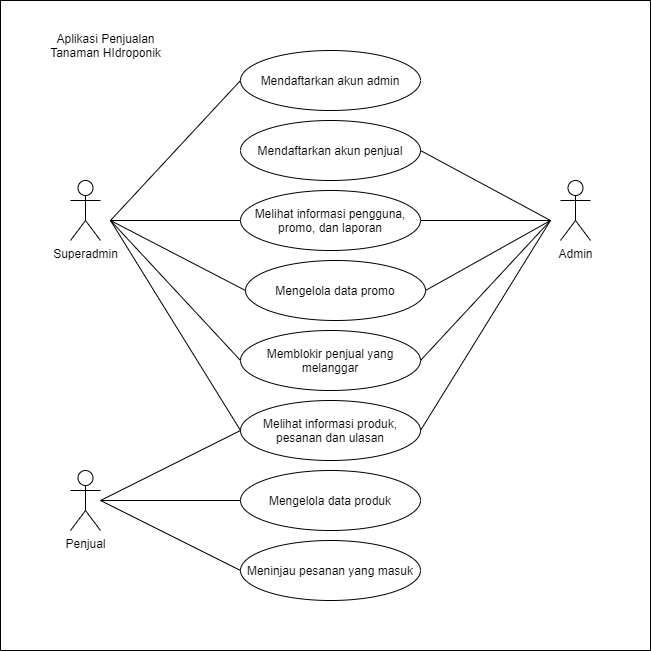
\includegraphics [width = 13cm, height= 13cm]{gambar/use_case_diagram}}
	\caption{\textit{Use Case Diagram}}
	\label{use_case_diagram}
\end{figure}

\par Gambar \ref*{use_case_diagram} merupakan\textit{ Use case diagram} yang menjelaskan interaksi antara superadmin, admin dan penjual dengan sistem aplikasi. Di mana level yang paling tinggi di sistem ini adalah superadmin yang bertindak untuk mendaftarkan admin, lalu nantinya para admin inilah yang bertugas mendaftarkan para penjual yang ingin menjual produknya di aplikasi AgriHub ini. Superadmin dan admin di sini dapat memantau informasi semua pengguna yang sudah terdaftar diaplikasi baik itu penjual maupun pembeli yang mendaftar lewat aplikasi Android dan dapat melihat produk-produk apa saja yang telah diunggah oleh para penjual, serta dapat menghapusnya jika dianggap tidak sesuai. Superadmin dan admin juga dapat melihat semua pesanan yang sudah terjadi antara penjual dengan pembeli, melihat ulasan dari pembeli terhadap produk yang dibeli dari penjual serta dapat mengadakan promo sesekali di aplikasinya dan dapat melihat laporan yang masuk dari pembeli terhadap penjual serta dapat mengambil tindakan seperti memblokir penjual tersebut dari sistem.
\newpage
\par Sedangkan dari sisi aktor penjual. Setelah penjual didaftarkan oleh admin, penjual harus memverifikasi emailnya terlebih dahulu sebelum bisa menggunakan aplikasinya. Baru setelah verifikasi email penjual dapat menggunakan aplikasinya untuk menambahkan produk yang ingin dijualnya, mengelolanya seperti mengubah dan menghapus produk, menerima pesanan dari pembeli dan mengubah statusnya dari belum menjadi diproses, dikirim dan sampai selesai. Penjual juga dapat melihat ulasan-ulasan dari pembeli terhadap pesanan dan produk yang ia jual di aplikasi.

% \subsection{\textit{Business Diagram}}
% \textit{Business diagram} merupakan diagram yang menggambarkan alur proses bisnis yang berjalan dari sebuah sistem. \textit{Business diagram} dapat membuat alur proses bisnis menjadi lebih sederhana sehingga mudah dipahami oleh semua orang. \textit{Business diagram} juga dapat dibuat secara umum dengan hanya berfokus pada proses bisnis inti saja. Pada rancangan \textit{business diagram} ini, proses bisnis inti terdiri dari :

% \begin{enumerate}
% 	\item Mendaftarkan diri sebagai penjual kepada admin
% 	\item Memverifikasi email yang sudah didaftarkan admin
% 	\item Menambahkan produk yang ingin dijual
% 	\item Menerima dan memproses pesanan.
% \end{enumerate}

% Untuk \textit{Business Diagram} dapat dilihat pada Gambar \ref{bisnis_diagram}.

% \begin{figure}[H]
% 	\centering
% 	{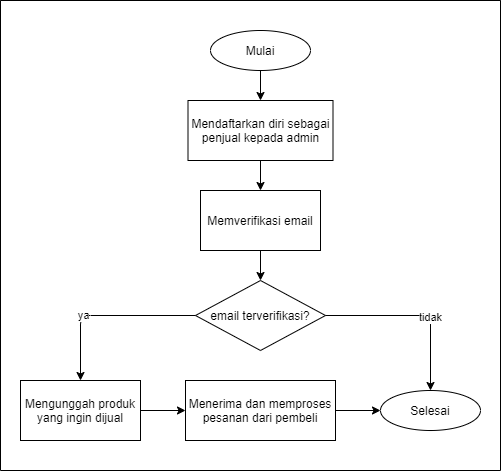
\includegraphics [width = 12cm, height= 10cm]{gambar/bisnis diagram baru}}
% 	\caption{\textit{Business Diagram}}
% 	\label{bisnis_diagram}
% \end{figure}

% Gambar 4.2 memperlihatkan alur bisnis di dalam sistem. Dimulai ketika pengguna ingin mendaftarkan diri sebagai penjual kepada admin, kemudian admin meminta datanya beserta email yang valid dari penjual untuk didaftarkan di sistem. Setelah datanya didaftarkan maka penjual harus memverifikasi emailnya terlebih dahulu sebelum bisa menggunakan aplikasi, setelah terverifikasi maka proses bisnis selanjutnya adalah penjual menjual produknya di dalam sistem. Tahapan tersebut penting agar produk dari penjual dapat dilihat dan dipesan oleh pembeli. Setelah pembeli membeli atau memesan produk, tahapan selanjutnya adalah penjual menerima dan memproses pesanan dari pembeli.

\subsection{\textit{Sequence Diagram}}
\textit{Sequence diagram} atau diagram urutan adalah sebuah diagram yang digunakan untuk menjelaskan dan menampilkan interaksi antar objek-objek dalam sebuah sistem secara terperinci. Selain itu \textit{sequence diagram} juga akan menampilkan pesan atau perintah yang dikirim, beserta waktu pelaksanaannya. Objek-objek yang berhubungan dengan berjalannya proses operasi biasanya diurutkan dari kiri ke kanan. Berikut merupakan \textit{sequence} diagram dalam penelitian ini :

\begin{enumerate}
	\item \textit{Sequence Diagram Login}
	\begin{figure}[H]
		\centering
		{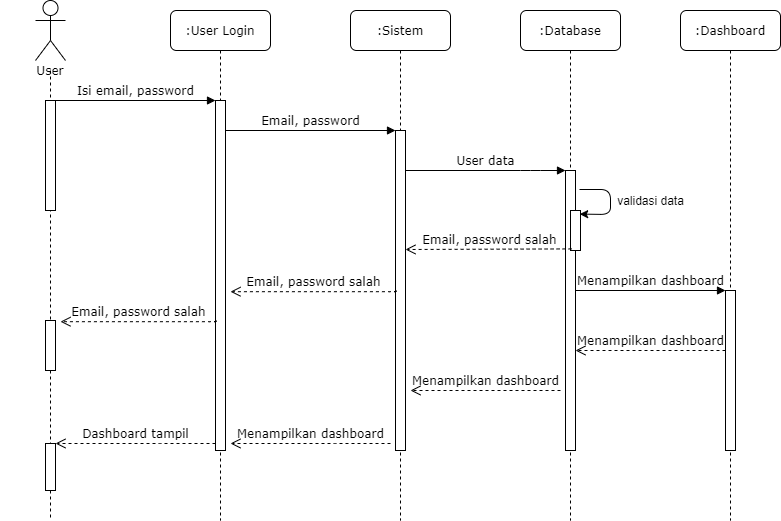
\includegraphics [width = 12cm, height= 7.6cm]{gambar/sequence/login}}
		\caption{\textit{Sequence Diagram Login}}
		\label{seq login}
	\end{figure}
	\par Gambar \ref*{seq login} memperlihatkan urutan interaksi ketika pengguna ingin \textit{login} ke dalam sistem. Pengguna mengisi \textit{email} dan \textit{password} pada halaman \textit{login}, kemudian sistem akan mengirimkan data tersebut ke \textit{database} untuk divalidasi apakah terdaftar atau tidak. Jika tidak terdaftar atau tidak sesuai maka sistem akan menampilkan pesan \textit{email} dan \textit{password} salah, tapi jika terdaftar dan sesuai maka sistem akan menampilkan \textit{dashboard} kepada pengguna.

	\item \textit{Sequence Diagram} Menu Produk
	\begin{figure}[H]
		\centering
		{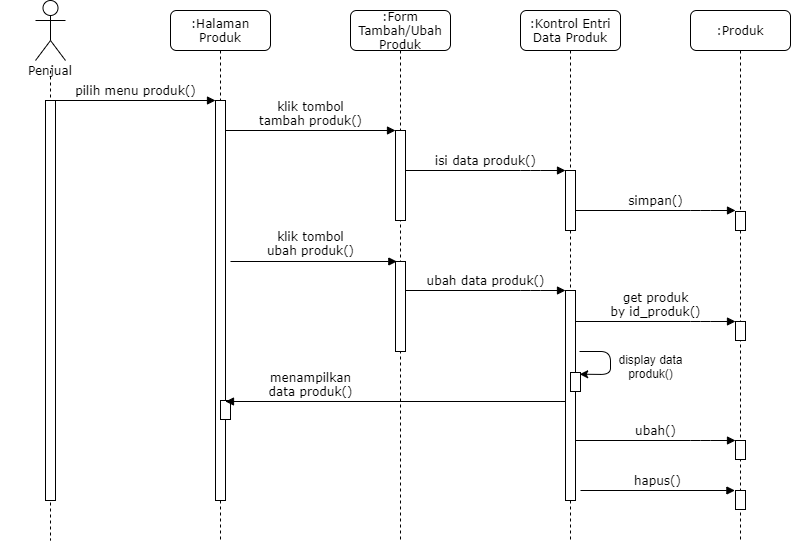
\includegraphics [width = 12cm, height= 7.35cm]{gambar/sequence/tambah, ubah, hapus produk}}
		\caption{\textit{Sequence Diagram} Menu Produk}
		\label{seq produk}
	\end{figure}
	\par Gambar \ref*{seq produk} memperlihatkan urutan interaksi ketika penjual mengakses menu produk, penjual dapat menambahkan produk dengan menklik tombol tambah dan mengisi data produk pada form yang tampil, kemudian sistem melakukan proses penyimpanan data ke dalam tabel produk. Jika penjual ingin mengubah atau menghapus produk dapat menklik tombol ubah di halaman produk, kemudian sistem akan memanggil data produk berdasarkan idnya dan menampilkan kembali data produknya setelah diubah atau dapat menklik tombol hapus maka sistem akan menghapus data produknya dari tabel produk.

	\item \textit{Sequence Diagram} Menu Pesanan
	\begin{figure}[H]
		\centering
		{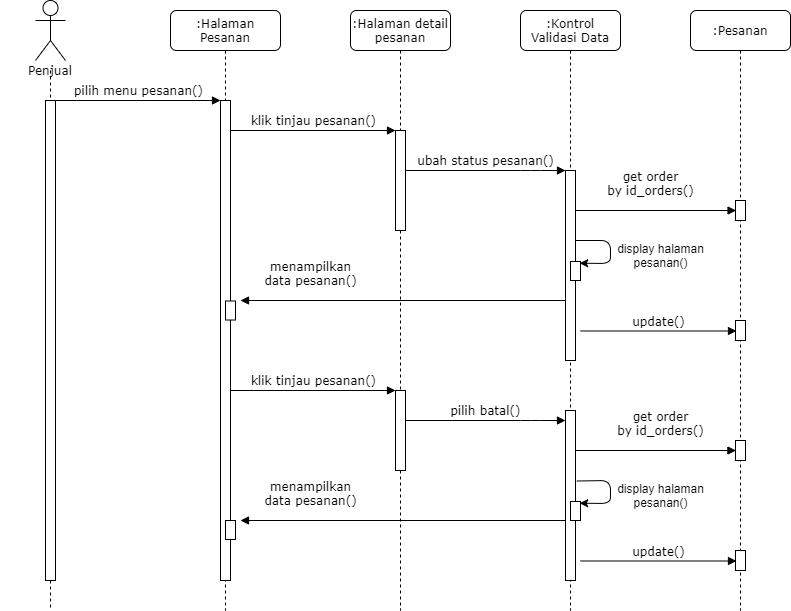
\includegraphics [width = 12cm, height= 7.35cm]{gambar/sequence/proses pesanan}}
		\caption{\textit{Sequence Diagram} Menu Pesanan}
		\label{seq pesanan}
	\end{figure}
	\par Gambar \ref*{seq pesanan} memperlihatkan urutan interaksi ketika penjual mengakses menu pesanan. Penjual dapat memproses pesanan yang masuk atau membatalkannya dengan menklik tombol tinjau pesanan, lalu mengisi ongkos kirim dan mengubah status pesanan menjadi diproses, dikirim atau selesai jika ingin memprosesnya, namun jika ingin membatalkannya dapat memilih batal. Kemudian sistem akan mencari data pesanan tersebut berdasarkan id\_order dan mengupdate data pesanannya lalu menampilkan kembali data pesanan pada halaman pesanan.

	\item \textit{Sequence Diagram} Menu Promo
	\begin{figure}[H]
		\centering
		{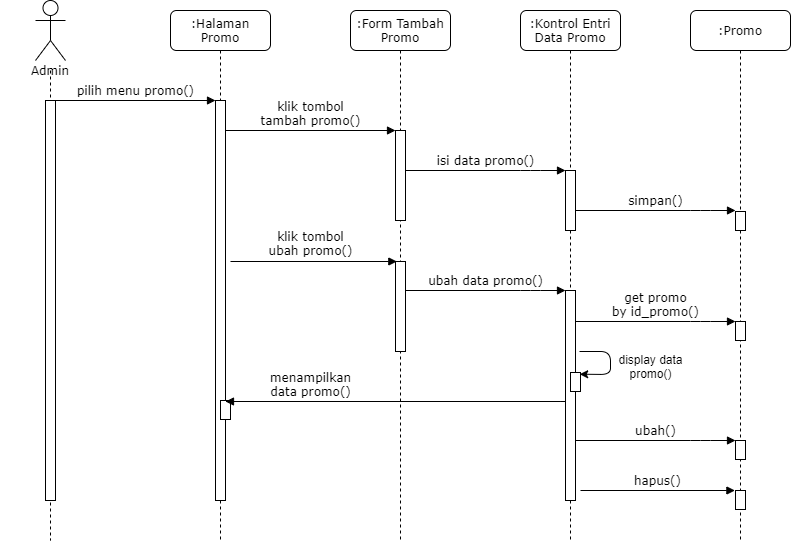
\includegraphics [width = 12cm, height= 8cm]{gambar/sequence/tambah, ubah, hapus promo}}
		\caption{\textit{Sequence Diagram} Menu Promo}
		\label{seq promo}
	\end{figure}
	\par Gambar \ref*{seq promo} memperlihatkan urutan interaksi ketika admin mengakses menu promo, admin dapat menambahkan promo dengan menklik tombol tambah dan mengisi data promo pada form yang tampil, kemudian sistem melakukan proses penyimpanan data ke dalam tabel promo. Jika admin ingin mengubah atau menghapus promo dapat menklik tombol ubah di halaman promo, kemudian sistem akan memanggil data promo berdasarkan idnya dan menampilkan kembali data promonya setelah diubah atau dapat menklik tombol hapus maka sistem akan menghapus datanya dari tabel promo.

	\newpage
	\item \textit{Sequence Diagram} Menu Pengguna
	\begin{figure}[H]
		\centering
		{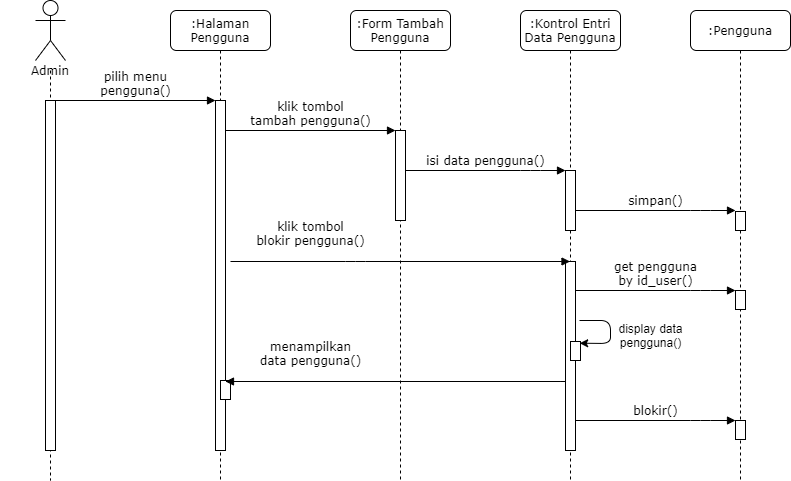
\includegraphics [width = 12cm, height= 8cm]{gambar/sequence/tambah, blokir pengguna}}
		\caption{\textit{Sequence Diagram} Menu Pengguna}
		\label{seq pengguna}
	\end{figure}
	\par Gambar \ref*{seq pengguna} memperlihatkan urutan interaksi ketika admin mengakses menu pengguna, admin dapat menambahkan pengguna baru dalam hal ini yaitu penjual dengan menklik tombol tambah dan mengisi data penjual pada form yang tampil, kemudian sistem akan menyimpan datanya ke dalam tabel pengguna. Jika admin ingin memblokir penjual dapat menekan tombol blokir maka sistem akan mencari data penjual tersebut berdasarkan id\_user dan mengubah status akunnya menjadi diblokir dan menampilkan kembali data pengguna pada halaman pengguna.

	\item \textit{Sequence Diagram} Menu Keluhan
	\begin{figure}[H]
		\centering
		{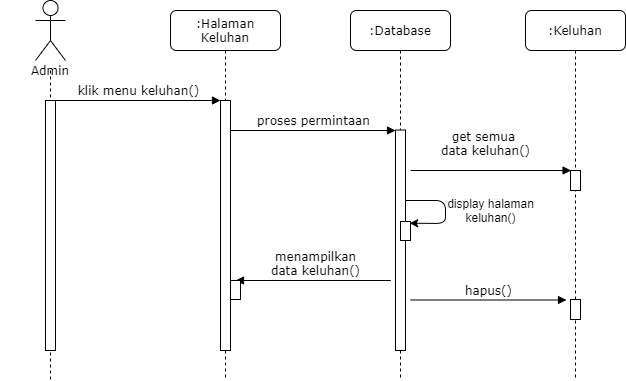
\includegraphics [width = 11cm, height= 6.7cm]{gambar/sequence/keluhan}}
		\caption{\textit{Sequence Diagram} Menu Keluhan}
		\label{seq keluhan}
	\end{figure}
	\par Gambar \ref*{seq keluhan} memperlihatkan urutan interaksi ketika admin mengakses menu keluhan. Admin dapat melihat keluhan dari pembeli dengan menklik menu keluhan, kemudian sistem akan mengirimkan permintaan ke \textit{database} untuk mendapatkan semua data keluhan dan menampilkannya pada halaman keluhan. Admin juga dapat menghapus keluhan dari pembeli jika dinilai asal-asalan dengan menekan tombol hapus maka sistem akan menghapusnya dari tabel keluhan.

	\item \textit{Sequence Diagram} Menu Ulasan
	\begin{figure}[H]
		\centering
		{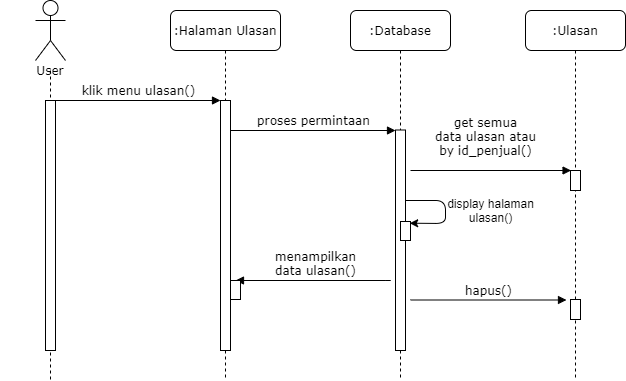
\includegraphics [width = 11cm, height= 8cm]{gambar/sequence/ulasan}}
		\caption{\textit{Sequence Diagram} Menu Ulasan}
		\label{seq ulasan}
	\end{figure}
	\par Gambar \ref*{seq ulasan} memperlihatkan urutan interaksi ketika user mengakses menu ulasan. User disini yaitu admin dan penjual dapat melihat ulasan dari pembeli dengan menklik menu ulasan, kemudian sistem akan mengirimkan permintaan ke \textit{database} untuk mendapatkan semua data ulasan bagi admin dan data ulasan berdasarkan id\_penjual bagi penjual lalu menampilkannya pada halaman ulasan. Admin dan penjual juga dapat menghapus ulasan dari pembeli jika dinilai mengandung kata tidak pantas dengan menekan tombol hapus maka sistem akan menghapusnya dari tabel ulasan.

	\newpage
	\item \textit{Sequence Diagram Update} Profil
	\begin{figure}[H]
		\centering
		{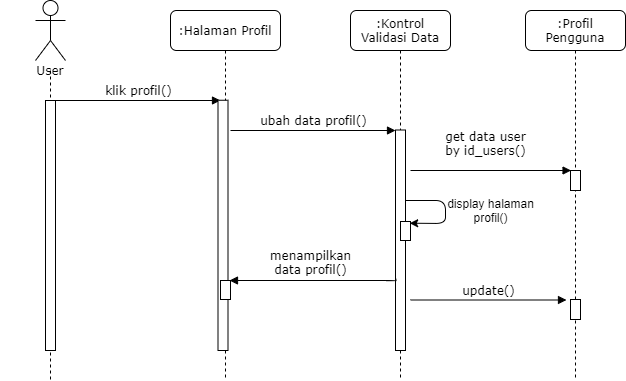
\includegraphics [width = 11cm, height= 8cm]{gambar/sequence/update profil}}
		\caption{\textit{Sequence Diagram Update} Profil}
		\label{seq profil}
	\end{figure}
	\par Gambar \ref*{seq profil} memperlihatkan urutan interaksi ketika \textit{user} ingin meng\textit{update} profil. \textit{User} dapat menklik profil, kemudian mengubah data profilnya lalu sistem akan mencari data \textit{user} tersebut berdasarkan id\_user yang \textit{login} dan meng\textit{update} data profilnya. Kemudian sistem menampilkan kembali data profil \textit{user} yang telah ter\textit{update}.
\end{enumerate}
	
\subsection{\textit{Activity Diagram}}
\textit{Activity Diagram} merupakan salah satu diagram yang menggambarkan langkah-langkah alur yang lebih rinci dari sistem. \textit{Activity Diagram} mempunyai titik mulai dan titik selesai yang di dalamnya menjelaskan berbagai alur kerja sistem secara beruntun. Biasanya \textit{Activity
Diagram} digunakan oleh pengembang aplikasi untuk memahami alur program yang akan dibuat. Berikut merupakan \textit{activity} diagram dalam penelitian ini :

\newpage

\begin{enumerate}
	\item \textit{Activity Diagram} Masuk Akun
	\begin{figure}[H]
		\centering
		{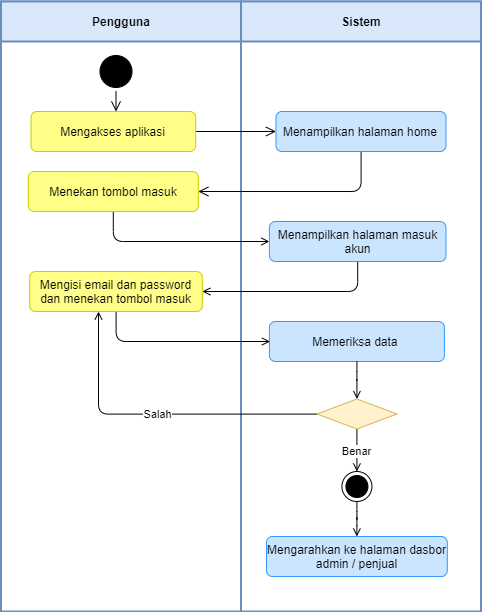
\includegraphics [width = 8cm, height= 10.5cm]{gambar/activity diagram/masuk akun}}
		\caption{\textit{Activity Diagram} Masuk Akun}
		\label{masuk akun}
	\end{figure}
	\par Gambar \ref*{masuk akun} memperlihatkan aktivitas ketika pengguna ingin masuk akun atau \textit{login} ke dalam sistem. Pengguna mengakses aplikasi terlebih dahulu dan menekan tombol masuk lalu mengisi data seperti \textit{email} dan \textit{password} yang kemudian akan diperiksa oleh sistem.

	\item \textit{Activity Diagram} Melihat Produk
	\begin{figure}[H]
		\centering
		{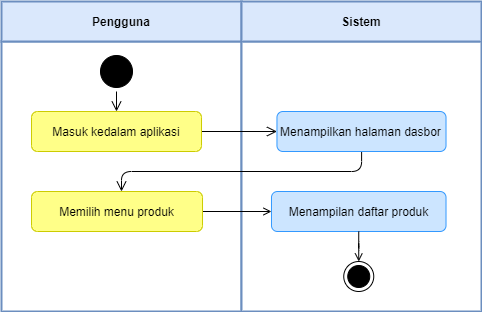
\includegraphics [width = 8cm, height= 6cm]{gambar/activity diagram/lihat produk}}
		\caption{\textit{Activity Diagram} Melihat Produk}
		\label{lihat produk}
	\end{figure}
	\par Gambar \ref*{lihat produk} memperlihatkan aktivitas ketika pengguna baik itu admin maupun penjual ketika hendak melihat daftar produk. Pengguna harus terlebih dahulu masuk ke dalam aplikasi lalu memilih menu produk, maka akan tampil halaman daftar semua produk yang dijual disistem bagi sisi admin dan akan tampil halaman daftar produk yang ia jual bagi sisi penjual.

	\item \textit{Activity Diagram} Menambahkan Produk
	\begin{figure}[H]
		\centering
		{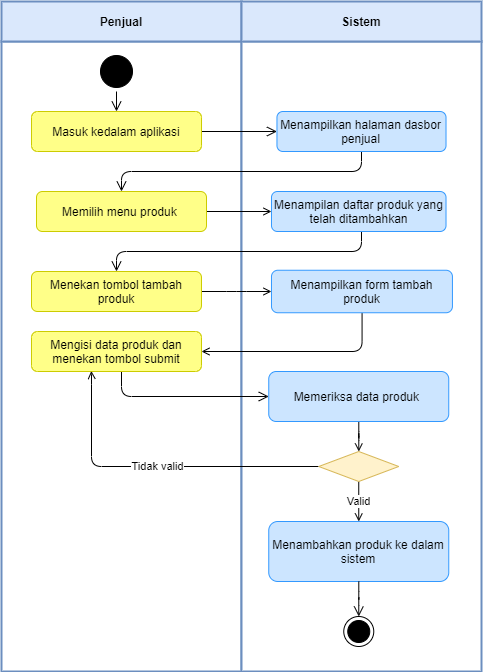
\includegraphics [width = 8cm, height= 11cm]{gambar/activity diagram/jual produk}}
		\caption{\textit{Activity Diagram} Menambahkan Produk}
		\label{jual produk}
	\end{figure}
	\par Gambar \ref*{jual produk} memperlihatkan aktivitas ketika penjual hendak menambahkan produk ke dalam sistem. Aktivitas ini hanya bisa dilakukan oleh penjual dan sudah melakukan aktivitas masuk akun (\textit{login}). Pada halaman produk penjual dapat menambahkan produk dengan menekan tombol tambah, lalu sistem akan menampilkan \textit{form} data produk untuk diisi oleh penjual. Setelah penjual mengisi semua data mengenai produk baru lalu menekan tombol \textit{submit}, maka sistem akan memvalidasi datanya. Apabila bila data yang di \textit{input} valid maka proses tambah produk berhasil dan data tersebut akan disimpan di sistem.

	\newpage
	\item \textit{Activity Diagram} Mengubah atau Menghapus Produk
	\begin{figure}[H]
		\centering
		{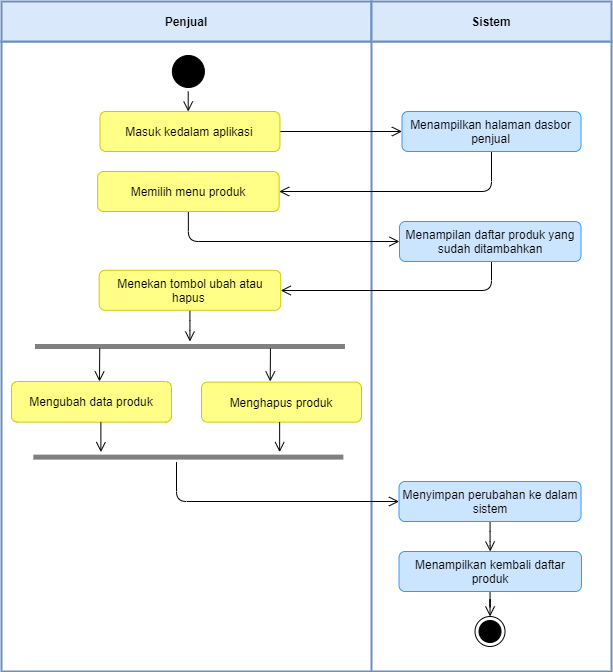
\includegraphics [width = 8cm, height= 11cm]{gambar/activity diagram/ubah atau hapus produk}}
		\caption{\textit{Activity Diagram} Mengubah atau Menghapus Produk}
		\label{ubah atau hapus produk}
	\end{figure}
	\par Gambar \ref*{ubah atau hapus produk} memperlihatkan aktivitas ketika penjual hendak mengubah atau menghapus produk yang dia jual di sistem. Penjual dapat mengubah data produk seperti gambar, nama, harga, stok dan data lainnya atau penjual bisa juga menghapus produknya dari sistem jika diinginkan.

	\item \textit{Activity Diagram} Melihat Pesanan
	\begin{figure}[H]
		\centering
		{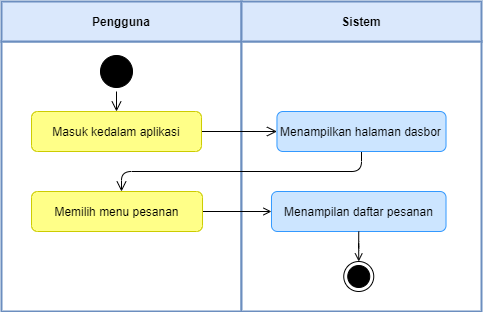
\includegraphics [width = 8cm, height= 6cm]{gambar/activity diagram/lihat pesanan}}
		\caption{\textit{Activity Diagram} Melihat Pesanan}
		\label{lihat pesanan}
	\end{figure}
	\par Gambar \ref*{lihat pesanan} memperlihatkan aktivitas ketika pengguna baik itu admin maupun penjual ketika hendak melihat daftar pesanan. Pengguna harus terlebih dahulu masuk ke dalam aplikasi lalu memilih menu pesanan, maka akan tampil halaman daftar semua pesanan yang sudah terjadi disistem bagi sisi admin dan akan tampil halaman daftar pesanan yang dia terima dari pembeli bagi sisi penjual.

	\item \textit{Activity Diagram} Mengubah Status Pesanan
	\begin{figure}[H]
		\centering
		{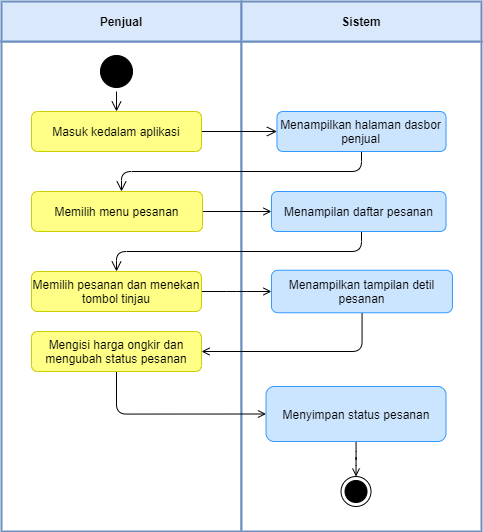
\includegraphics [width = 8cm, height= 11cm]{gambar/activity diagram/ubah status pesanan}}
		\caption{\textit{Activity Diagram} Mengubah Status Pesanan}
		\label{ubah status pesanan}
	\end{figure}
	\par Gambar \ref*{ubah status pesanan} memperlihatkan aktivitas ketika penjual ingin mengubah status pesanan dari pembeli. Penjual memilih terlebih dahulu pesanan yang ingin diproses lalu menekan tombol tinjau dan mengisi harga ongkos kirim pesanan tersebut serta mengubah status pesanannya dari belum menjadi diproses, dikirim, sampai selesai. Penjual juga bisa membatalkan pesanannya dengan mengubah status pesanan menjadi batal.

	\newpage
	\item \textit{Activity Diagram} Membuat Promo
	\begin{figure}[H]
		\centering
		{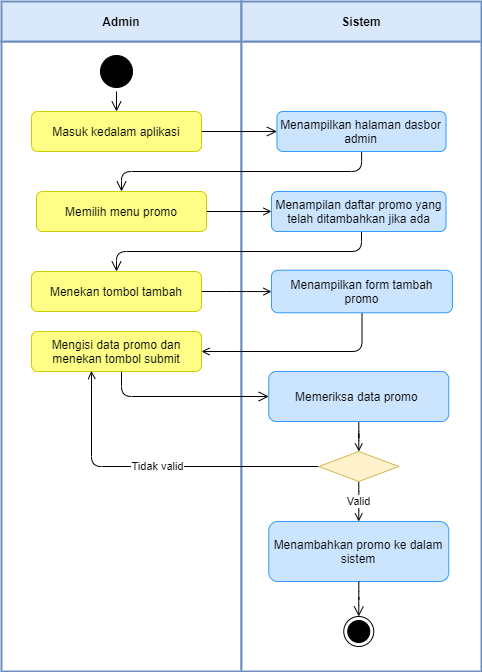
\includegraphics [width = 8cm, height= 12cm]{gambar/activity diagram/buat promo}}
		\caption{\textit{Activity Diagram} Membuat Promo}
		\label{buat promo}
	\end{figure}
	\par Gambar \ref*{buat promo} memperlihatkan aktivitas ketika admin ingin membuat promo di aplikasi. Admin masuk ke aplikasi terlebih dahulu, lalu memilih menu promo dan menekan tombol tambah. Kemudian mengisi data promo seperti gambar, nama promo, potongan, awal periode dan akhir periode. Setelah itu menekan tombol \textit{submit} maka sistem akan memeriksa datanya. Apabila data yang di \textit{input} valid maka proses pembuatan promo berhasil dan promo tersebut dapat digunakan oleh penjual nantinya.

	\newpage
	\item \textit{Activity Diagram} Mengubah atau Menghapus Promo
	\begin{figure}[H]
		\centering
		{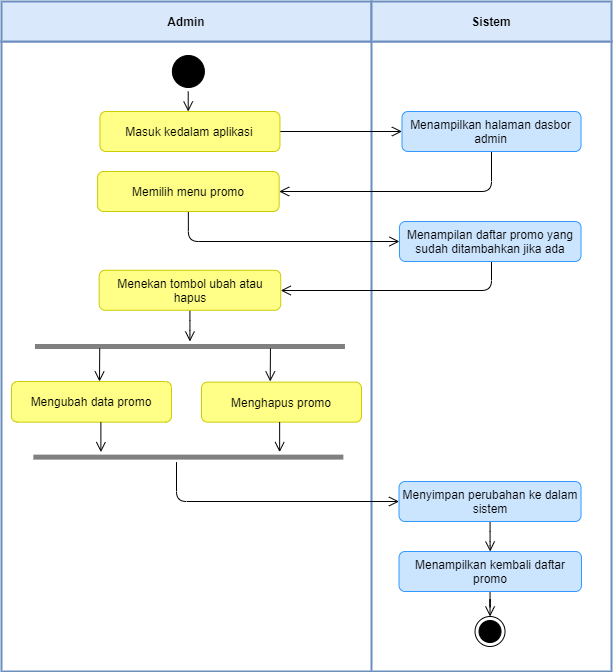
\includegraphics [width = 8cm, height= 11cm]{gambar/activity diagram/ubah atau hapus promo}}
		\caption{\textit{Activity Diagram} Mengubah atau Menghapus Promo}
		\label{ubah atau hapus promo}
	\end{figure}
	\par Gambar \ref*{ubah atau hapus promo} memperlihatkan aktivitas ketika admin hendak mengubah atau menghapus promo yang sedang berlangsung. Admin dapat mengubah data mengenai promo atau menghapusnya. Promo yang sudah melewati tanggal akhir periode akan terhapus otomatis di sistem.

	\item \textit{Activity Diagram} Melihat Pengguna
	\begin{figure}[H]
		\centering
		{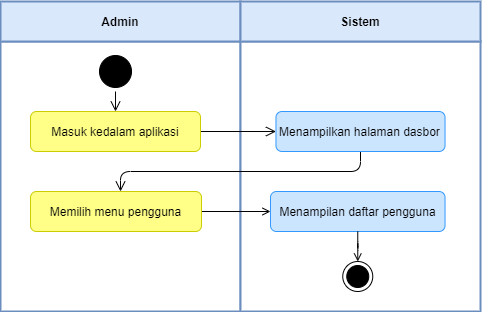
\includegraphics [width = 8cm, height= 6cm]{gambar/activity diagram/lihat pengguna}}
		\caption{\textit{Activity Diagram} Melihat Pengguna}
		\label{lihat pengguna}
	\end{figure}
	\par Gambar \ref*{lihat pengguna} memperlihatkan aktivitas ketika admin ingin melihat semua daftar pengguna yang sudah terdaftar disistem. Admin dapat melakukannya dengan masuk ke aplikasi dan memilih menu pengguna maka akan tampil daftar semua pengguna yang sudah terdaftar disistem baik itu admin, penjual maupun pembeli yang mendaftar lewat aplikasi Android.

	\item \textit{Activity Diagram} Mendaftarkan Akun Penjual
	\begin{figure}[H]
		\centering
		{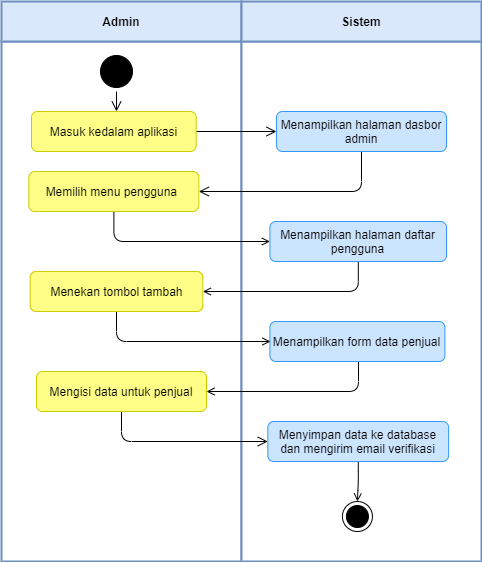
\includegraphics [width = 8cm, height= 11cm]{gambar/activity diagram/daftar akun penjual}}
		\caption{\textit{Activity Diagram} Masuk Akun Penjual}
		\label{daftar akun penjual}
	\end{figure}
	\par Gambar \ref*{daftar akun penjual} memperlihatkan aktivitas ketika admin ingin mendaftarkan akun penjual.
	Admin masuk ke aplikasi lalu memilih menu pengguna dan menekan tombol tambah. Kemudian mengisi data penjual seperti nama, \textit{username, email, password}, nomor hp, alamat dan menekan tombol \textit{submit}. Maka sistem akan menyimpan data penjual di \textit{database} dan mengirimkan \textit{email} verifikasi kepada penjual. Penjual harus memverifikasi \textit{email} tersebut agar dapat menggunakan akun yang sudah didaftarkan admin di aplikasi.

	\newpage
	\item \textit{Activity Diagram} Memblokir Akun Penjual
	\begin{figure}[H]
		\centering
		{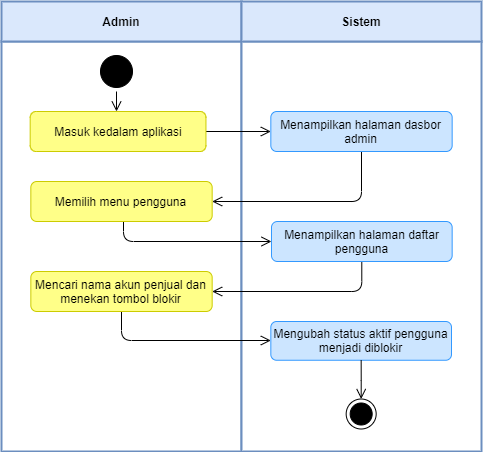
\includegraphics [width = 8cm, height= 10cm]{gambar/activity diagram/blokir penjual}}
		\caption{\textit{Activity Diagram} Memblokir Akun Penjual}
		\label{blokir penjual}
	\end{figure}
	\par Gambar \ref*{blokir penjual} memperlihatkan aktivitas ketika admin hendak memblokir salah satu akun penjual. Admin harus terlebih dahulu masuk ke dalam aplikasi, lalu memilih menu pengguna, kemudian mencari pengguna yang ingin diblokir dan menekan tombol blokir. Maka sistem akan mengubah status akun penjual tersebut menjadi diblokir dan penjual tersebut tidak bisa lagi masuk ke dalam aplikasi sampai admin mengubah status akunnya kembali.

	\item \textit{Activity Diagram} Melihat Keluhan
	\begin{figure}[H]
		\centering
		{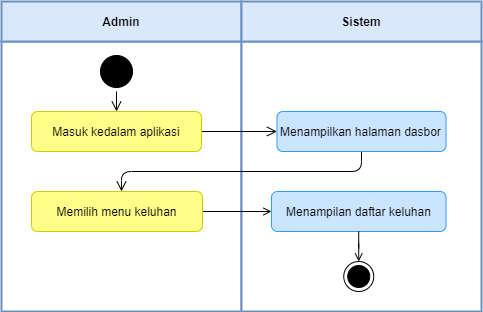
\includegraphics [width = 8cm, height= 6cm]{gambar/activity diagram/lihat keluhan}}
		\caption{\textit{Activity Diagram} Melihat Keluhan}
		\label{lihat keluhan}
	\end{figure}
	\par Gambar \ref*{lihat keluhan} memperlihatkan aktivitas ketika admin ingin melihat semua keluhan yang masuk dari para pembeli terhadap penjual yang terdaftar disistem. Admin dapat melakukannya dengan masuk ke aplikasi dan memilih menu keluhan maka akan tampil daftar semua keluhan yang dikirim oleh pembeli terhadap penjual.

	\item \textit{Activity Diagram} Melihat Ulasan Produk
	\begin{figure}[H]
		\centering
		{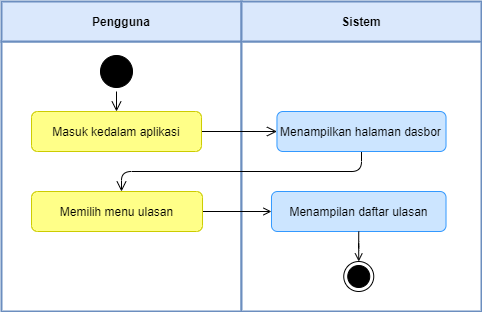
\includegraphics [width = 8cm, height= 6cm]{gambar/activity diagram/lihat ulasan}}
		\caption{\textit{Activity Diagram} Melihat Ulasan Produk}
		\label{lihat ulasan}
	\end{figure}
	\par Gambar \ref*{lihat ulasan} memperlihatkan aktivitas ketika pengguna ingin melihat daftar ulasan. Pengguna masuk ke dalam aplikasi lalu menekan tombol ulasan, maka akan tampil halaman daftar semua ulasan yang ada disistem bagi sisi admin dan akan tampil halaman daftar ulasan yang dia terima dari pembelinya bagi sisi penjual.

	\newpage
	\item \textit{Activity Diagram} Mengubah Profil Akun
	\begin{figure}[H]
		\centering
		{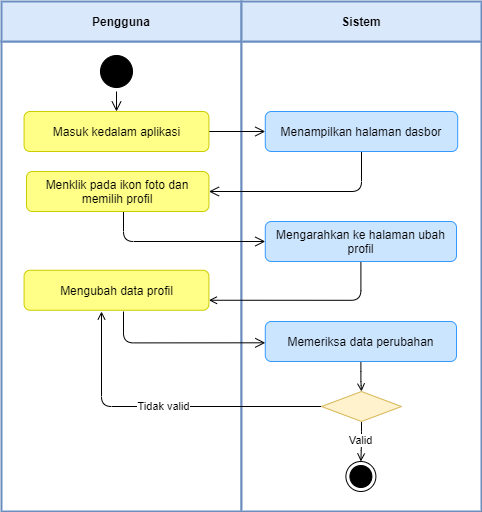
\includegraphics [width = 8cm, height= 9.5cm]{gambar/activity diagram/ubah profil}}
		\caption{\textit{Activity Diagram} Mengubah Profil Akun}
		\label{ubah profil}
	\end{figure}
	\par Gambar \ref*{ubah profil} memperlihatkan aktivitas ketika pengguna ingin mengubah profil akunnya. Pengguna masuk ke dalam aplikasi lalu menekan ikon foto dan memilih profil, maka akan diarahkan ke halaman ubah profil. Pengguna dapat mengubah data akunnya seperti foto profil, nama, email, nomor hp, alamat dan \textit{password}. Setelah selesai melakukan perubahan dan menekan tombol simpan, maka sistem akan memeriksa data perubahannya. Jika data \textit{input}nya valid maka akan disimpan di sistem.
\end{enumerate}

\subsection{\textit{Entity Relationship Diagram}}
\textit{Entity Relationship Diagram} (ERD) merupakan diagram yang menggambarkan hubungan antar data-data yang ada disistem yang saling berelasi satu sama yang lain. \textit{Entity Relationship Diagram} (ERD) dapat dilihat pada Gambar \ref{erd} berikut ini.
\begin{landscape}
	\begin{figure}[H]
		\centering
		{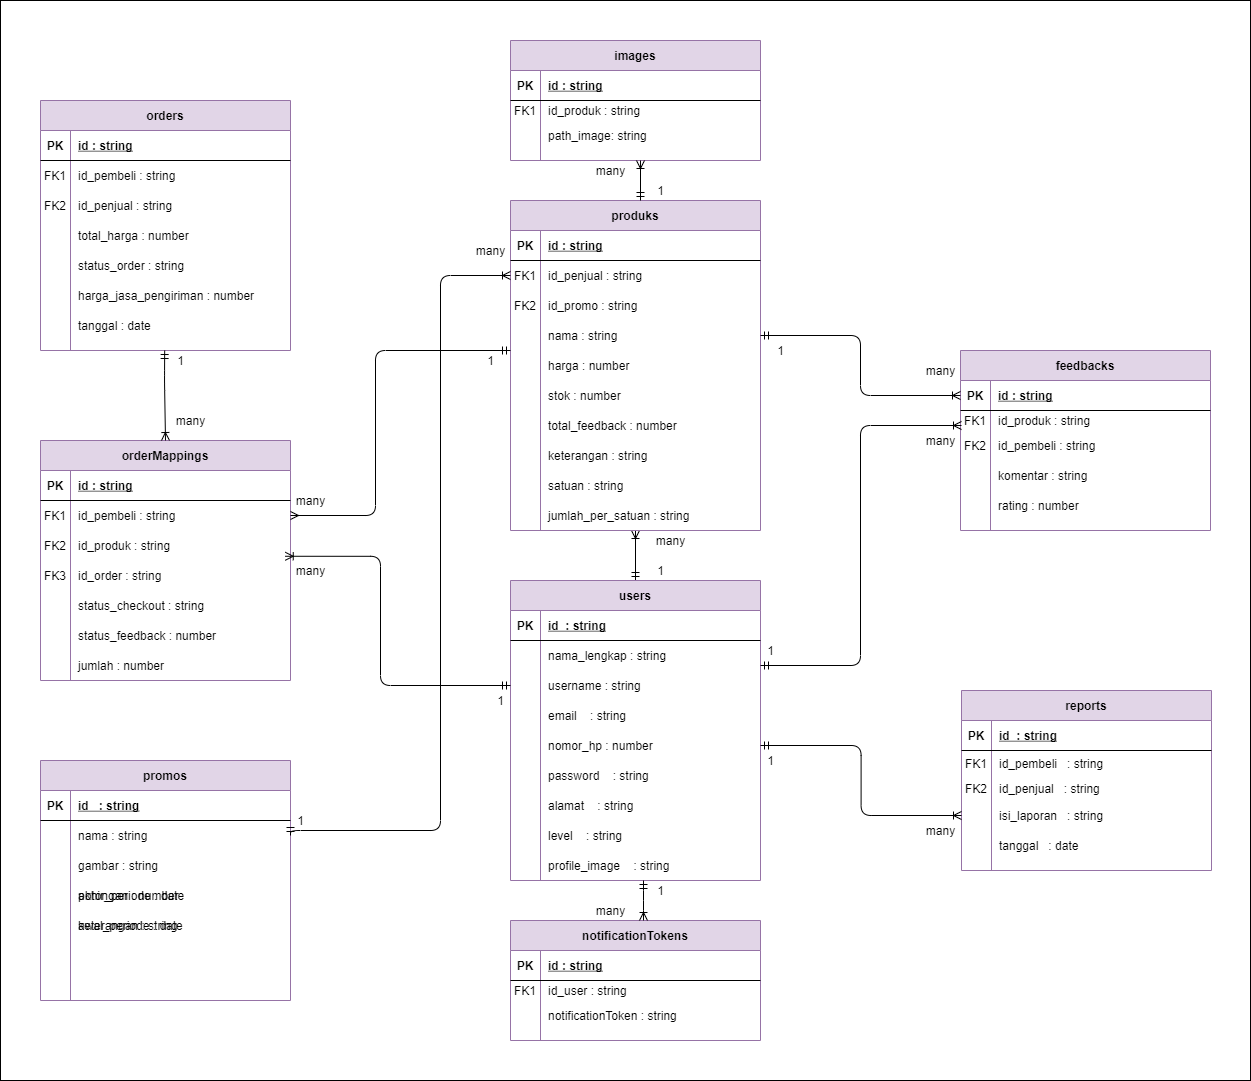
\includegraphics [width = 22cm, height= 13cm]{gambar/erd}}
		\caption{\textit{Entity Relationship Diagram}}
		\label{erd}
	\end{figure}
\end{landscape}

ERD yang dibuat pada penelitian ini mempunyai 9 entitas. Tiap entitas mempunyai atributnya masing-masing. Relasi antar entitas di dalam sistem ini memiliki kardinalitas (derajat) \textit{one to many}.  Adapun 9 entitas tersebut yang terdiri dari :

\begin{enumerate}
	\item Entitas \textit{users}
	\par Entitas ini akan menyimpan data semua pengguna di dalam aplikasi. Pada entitas \textit{users} terdapat 9 atribut yaitu : id, nama\_lengkap, \textit{username}, email, nomor\_hp, \textit{password}, alamat, level, dan \textit{profile\_image} . Atribut id akan menjadi \textit{primary key} serta di dalam entitas ini tidak memiliki \textit{foreign key}.
	\item Entitas \textit{notificationTokens}
	\par Entitas ini akan menyimpan data token ketika pengguna masuk ke dalam aplikasi berbasis Android. Pada entitas \textit{notificationTokens} terdapat 3 atribut yaitu : id, \textit{notificationToken}, dan id\_user . Atribut id akan menjadi \textit{primary key} serta id\_user dari entitas \textit{users} akan menjadi \textit{foreign key}.
	\item Entitas \textit{produks}
	\par Entitas ini akan menyimpan data produk yang akan ditambahkan oleh penjual. Pada entitas \textit{produks} terdapat 11 atribut yaitu : id, id\_penjual, id\_promo, nama, harga, stok, total\_feedback, keterangan, satuan jumlah\_per\_satuan. Atribut id akan menjadi \textit{primary key} serta id\_penjual dari entitas \textit{users} dan id\_promo dari entitas \textit{promos} akan menjadi \textit{foreign key}.
	\item Entitas \textit{images}
	\par Entitas ini akan menyimpan data yang berupa gambar dari entitas \textit{produks} dikarenakan satu data produk dapat memiliki lebih dari satu gambar. Pada entitas \textit{images} terdapat 3 atribut yaitu : id, id\_produk dan path\_image . Atribut id akan menjadi \textit{primary key} serta id\_produk dari entitas \textit{produks} akan menjadi \textit{foreign key}.
	\item Entitas \textit{promos}
	\par Entitas ini akan menyimpan data promo yang akan digunakan ketika suatu produk memiliki potongan harga atau promo. Pada entitas \textit{promos} terdapat 5 atribut yaitu : id, nama, gambar, potongan, awal\_periode, akhir\_periode, dan keterangan . Atribut id akan menjadi \textit{primary key} serta di dalam entitas ini tidak memiliki \textit{foreign key} apapun.
	\newpage
	\item Entitas \textit{orderMappings}
	\par Entitas ini akan menyimpan data setiap produk yang dipilih oleh pembeli ketika pembeli memesan produk atau melakukan checkout di dalam aplikasi berbasis Android. Pada entitas \textit{orderMappings} terdapat 7 atribut yaitu : id, id\_pembeli,
	id\_produk, id\_order, status\_checkout, status\_feedback, dan jumlah. Atribut id
	akan menjadi \textit{primary key} serta id\_pembeli dari entitas \textit{users}, id\_produk dari entitas \textit{produks} dan id\_order dari entitas \textit{orders} akan menjadi \textit{foreign key}.
	\item Entitas \textit{orders}
	\par Entitas ini akan menyimpan data pesanan pembeli yang berasal dari entitas \textit{orderMappings}. Pada entitas \textit{orders} terdapat 7 atribut yaitu : id, id\_pembeli, id\_penjual, total\_harga, status\_order harga\_jasa\_pengiriman, dan tanggal. Atribut id akan menjadi \textit{primary key} serta id\_pembeli dan id\_penjual dari entitas \textit{users} akan menjadi \textit{foreign key}.
	\item Entitas \textit{feedbacks}
	\par Entitas ini akan menyimpan data ulasan setiap produk yang diberikan oleh pembeli. Pada entitas \textit{feedbacks} terdapat 5 atribut yaitu : id, id\_produk,
	id\_pembeli, komentar, dan rating. Atribut id akan menjadi \textit{primary key} serta id\_pembeli dari entitas \textit{users} dan id\_produk dari entitas \textit{produks} akan menjadi \textit{foreign key}.
	\item Entitas \textit{reports}
	\par Entitas ini akan menyimpan data laporan tentang penjual yang dilakukan oleh pembeli. Pada entitas \textit{reports} terdapat 5 atribut yaitu : id, id\_penjual, id\_pembeli, isi\_laporan, dan tanggal. Atribut id akan menjadi \textit{primary key} serta id\_pembeli dan id\_penjual dari entitas \textit{users} akan menjadi \textit{foreign key}.
\end{enumerate}
	
\subsection{Antarmuka Aplikasi}
Antarmuka aplikasi adalah tampilan dari sebuah aplikasi yang dapat dilihat oleh pengguna. Antarmuka dalam aplikasi berbasis web ini terdiri dari bagian superadmin/admin dan bagian penjual. Dikarenakan terdapat beberapa perbedaan fitur aplikasi sesuai dengan jenis penggunanya.

\begin{enumerate}
	\item Antarmuka Aplikasi Bagian Superadmin/Admin
	
	Antarmuka aplikasi pada bagian superadmin/admin memiliki beberapa halaman yang dapat dilihat sebagai berikut :

	\newpage
	\begin{enumerate}[a.]
		\item Halaman Utama
		\par Halaman utama merupakan halaman yang pertama kali tampil ketika mengakses aplikasi web melalui \textit{browser}. Pada halaman utama ini terdapat 2 \textit{tab} navigasi dipojok kanan atas yaitu \textit{tab} informasi dan \textit{tab} masuk. Halaman utama dapat dilihat pada gambar \ref*{homepage}.
		\begin{figure}[H]
			\centering
			{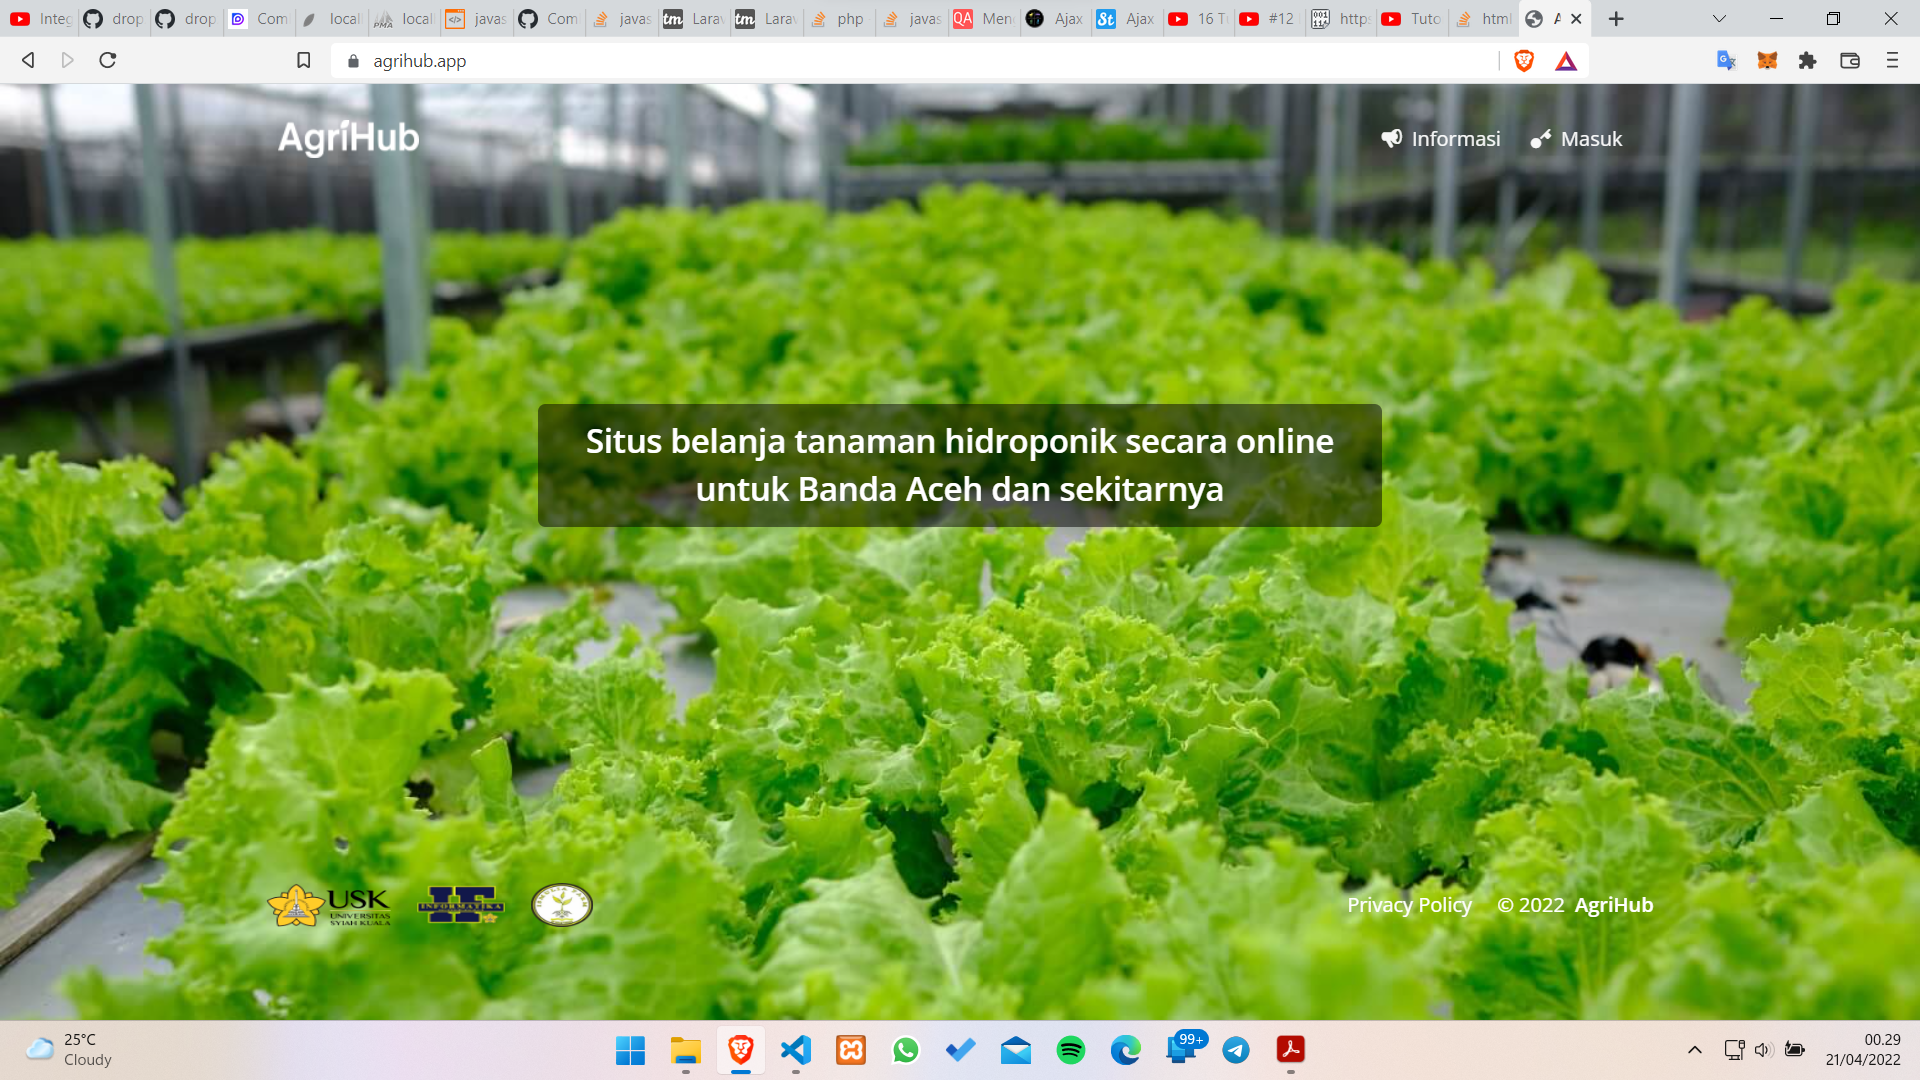
\includegraphics [width = 13cm, height= 7.5cm]{gambar/homepage}}
			\caption{Halaman Utama}
			\label{homepage}
		\end{figure}

		\item Halaman Masuk
		\par Halaman masuk merupakan halaman yang berfungsi untuk masuk ke dalam aplikasi dengan cara mengisi \textit{email} dan \textit{password} lalu menekan tombol Masuk yang berwarna hijau. Apabila data yang diisi benar, maka proses masuk akan berhasil. Halaman masuk dapat dilihat pada gambar \ref*{login}.
		\begin{figure}[H]
			\centering
			{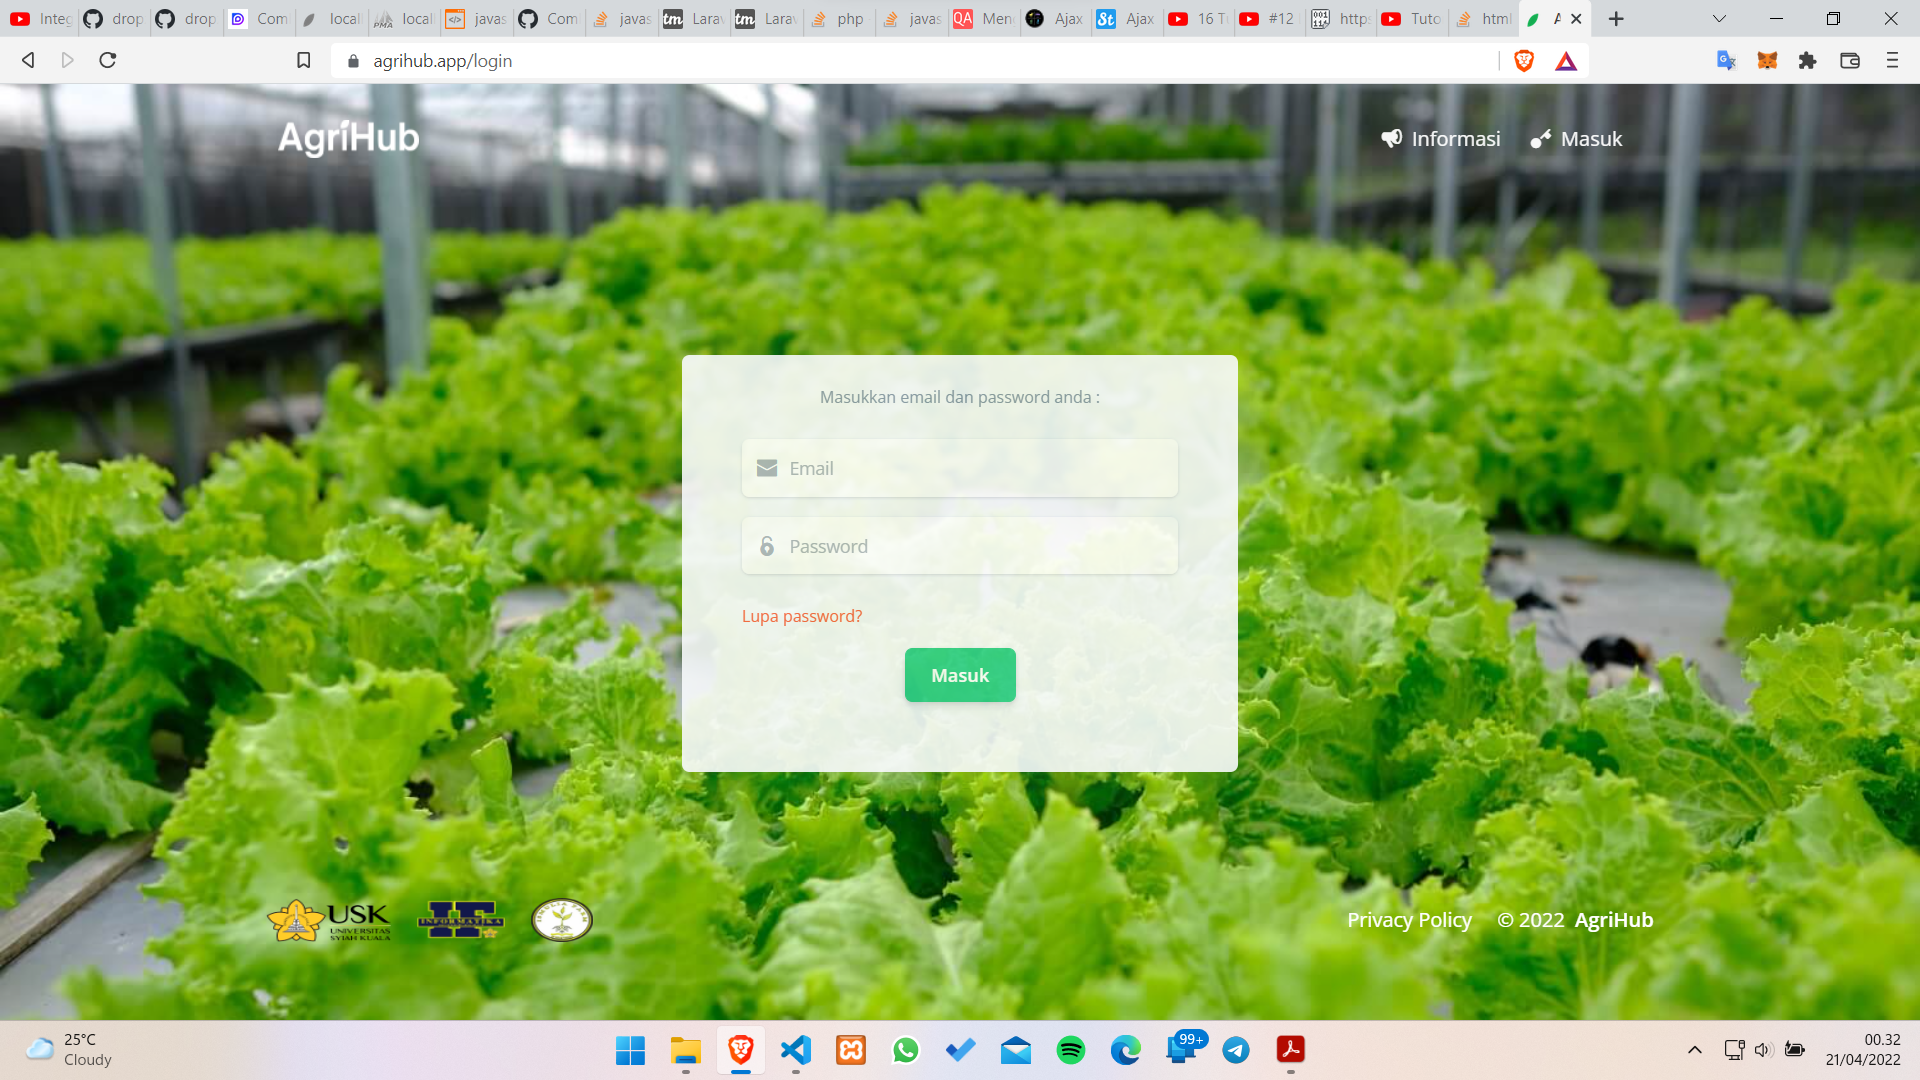
\includegraphics [width = 13cm, height= 7.5cm]{gambar/login}}
			\caption{Halaman Masuk}
			\label{login}
		\end{figure}
	
		\item Halaman Dasbor
		\par Setelah berhasil masuk ke aplikasi, maka akan tampil halaman dasbor. Halaman ini berisi informasi data jumlah produk yang sudah diunggah oleh para penjual, jumlah pesanan yang sudah terjadi di aplikasi, jumlah promo yang sedang berlangsung, jumlah pengguna yang sudah terdaftar di aplikasi, jumlah laporan yang masuk dari pembeli, dan jumlah ulasan yang sudah diberikan oleh pembeli terhadap produk yang dijual oleh penjual. Serta ditampilkan grafik jumlah pesanan yang selesai dan batal perbulannya dari para penjual, dan grafik jumlah produk baru yang diunggah oleh para penjual selama 6 bulan terakhir serta grafik jumlah admin, penjual dan pembeli. Halaman dasbor admin dapat dilihat pada gambar \ref*{dashboard_admin}.
		\begin{figure}[H]
			\centering
			{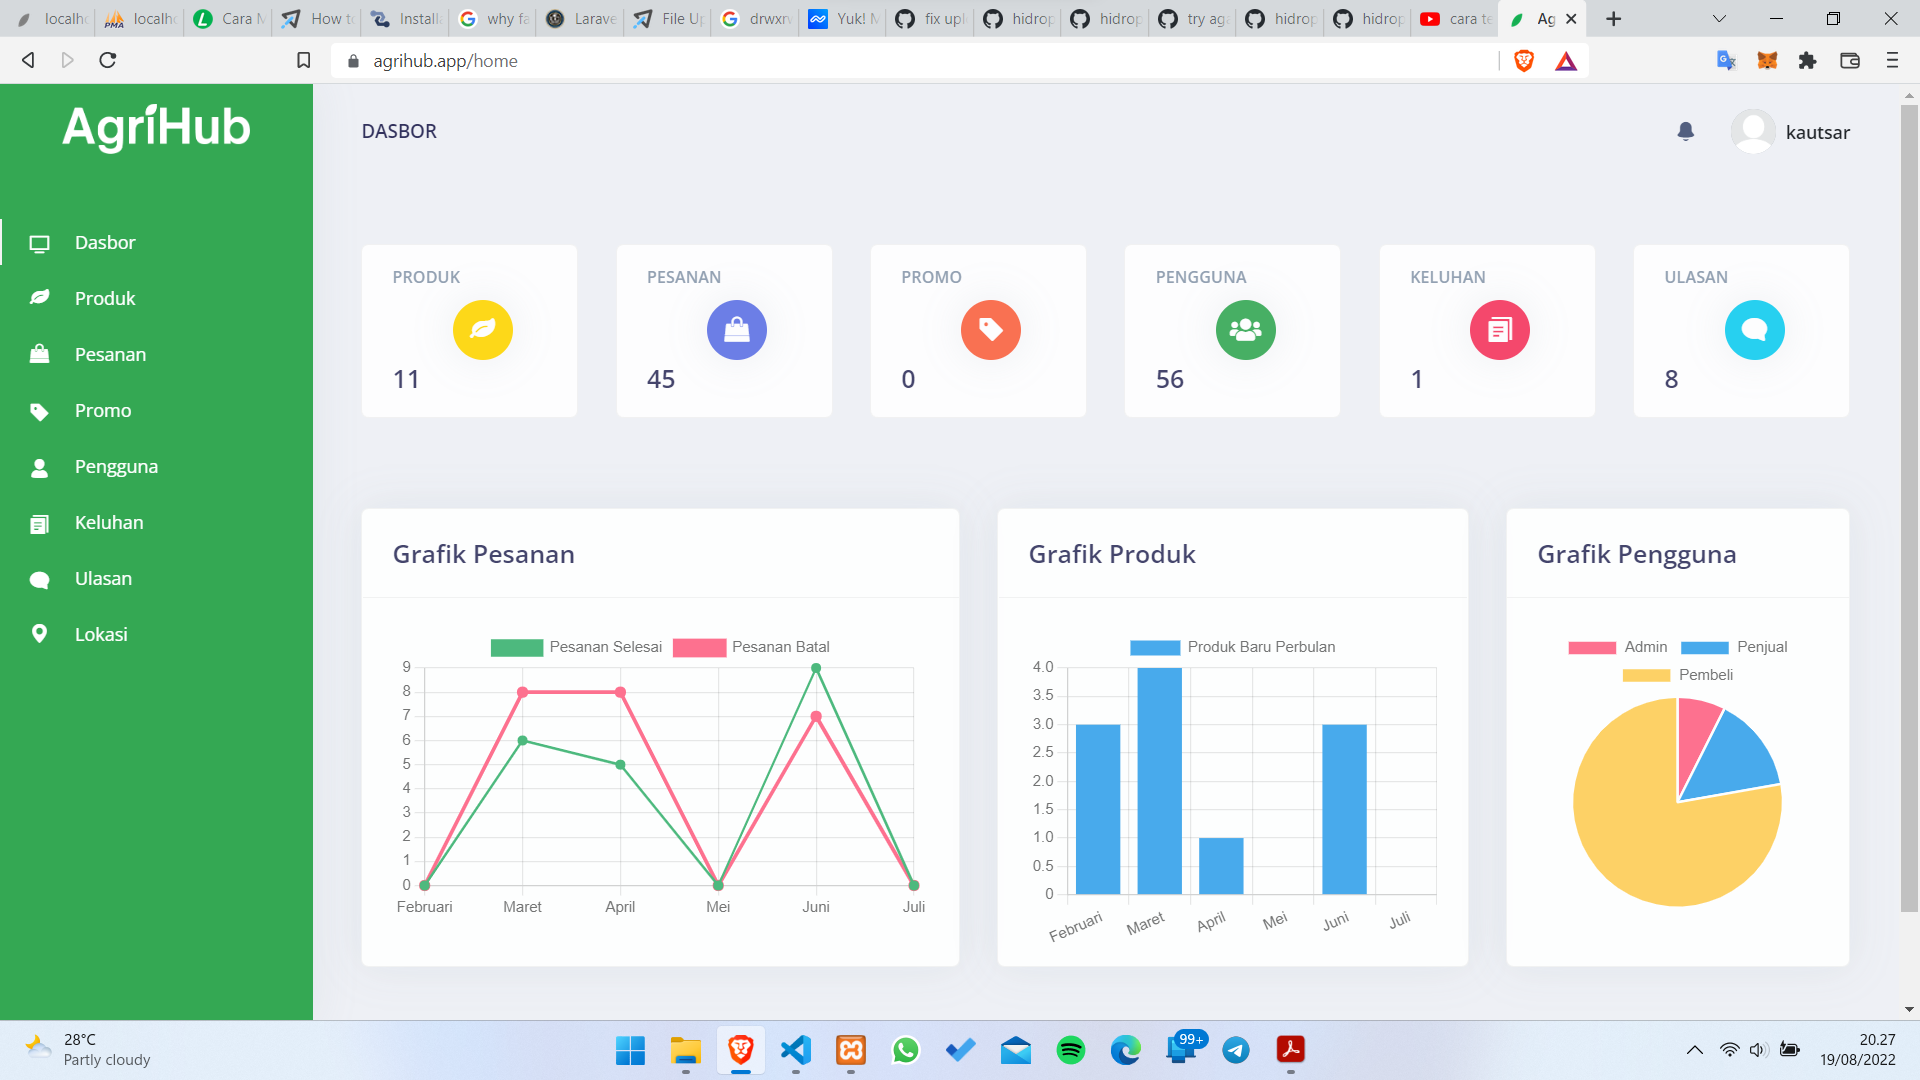
\includegraphics [width = 13cm, height= 7.5cm]{gambar/admin/dashboard_admin}}
			\caption{Halaman Dasbor pada sisi Admin}
			\label{dashboard_admin}
		\end{figure}

		\item Halaman Produk
		\par Pada halaman produk, admin dapat melihat informasi mengenai produk seperti id produk, gambar produk, nama produk dan lainnya. Admin juga dapat melakukan pencarian produk tertentu dengan memasukkan kata kunci di kolom cari produk, serta dapat memfilter produk berdasarkan satuannya dan menampilkan produk per halaman sebanyak 5, 10, atau 25 data. Dikarenakan gambar produk bisa lebih dari 1 maka admin dapat melihat gambar produk lainnya beserta dengan keterangan produk dan jumlah/satuannya dengan menekan tombol Lihat. Admin juga dapat menghapus produk penjual jika diperlukan dengan menekan tombol Hapus. Halaman produk dan tampilan detail produk dapat dilihat pada gambar \ref*{produk_admin} dan \ref*{lihat_produk_admin}.
		\begin{figure}[H]
			\centering
			{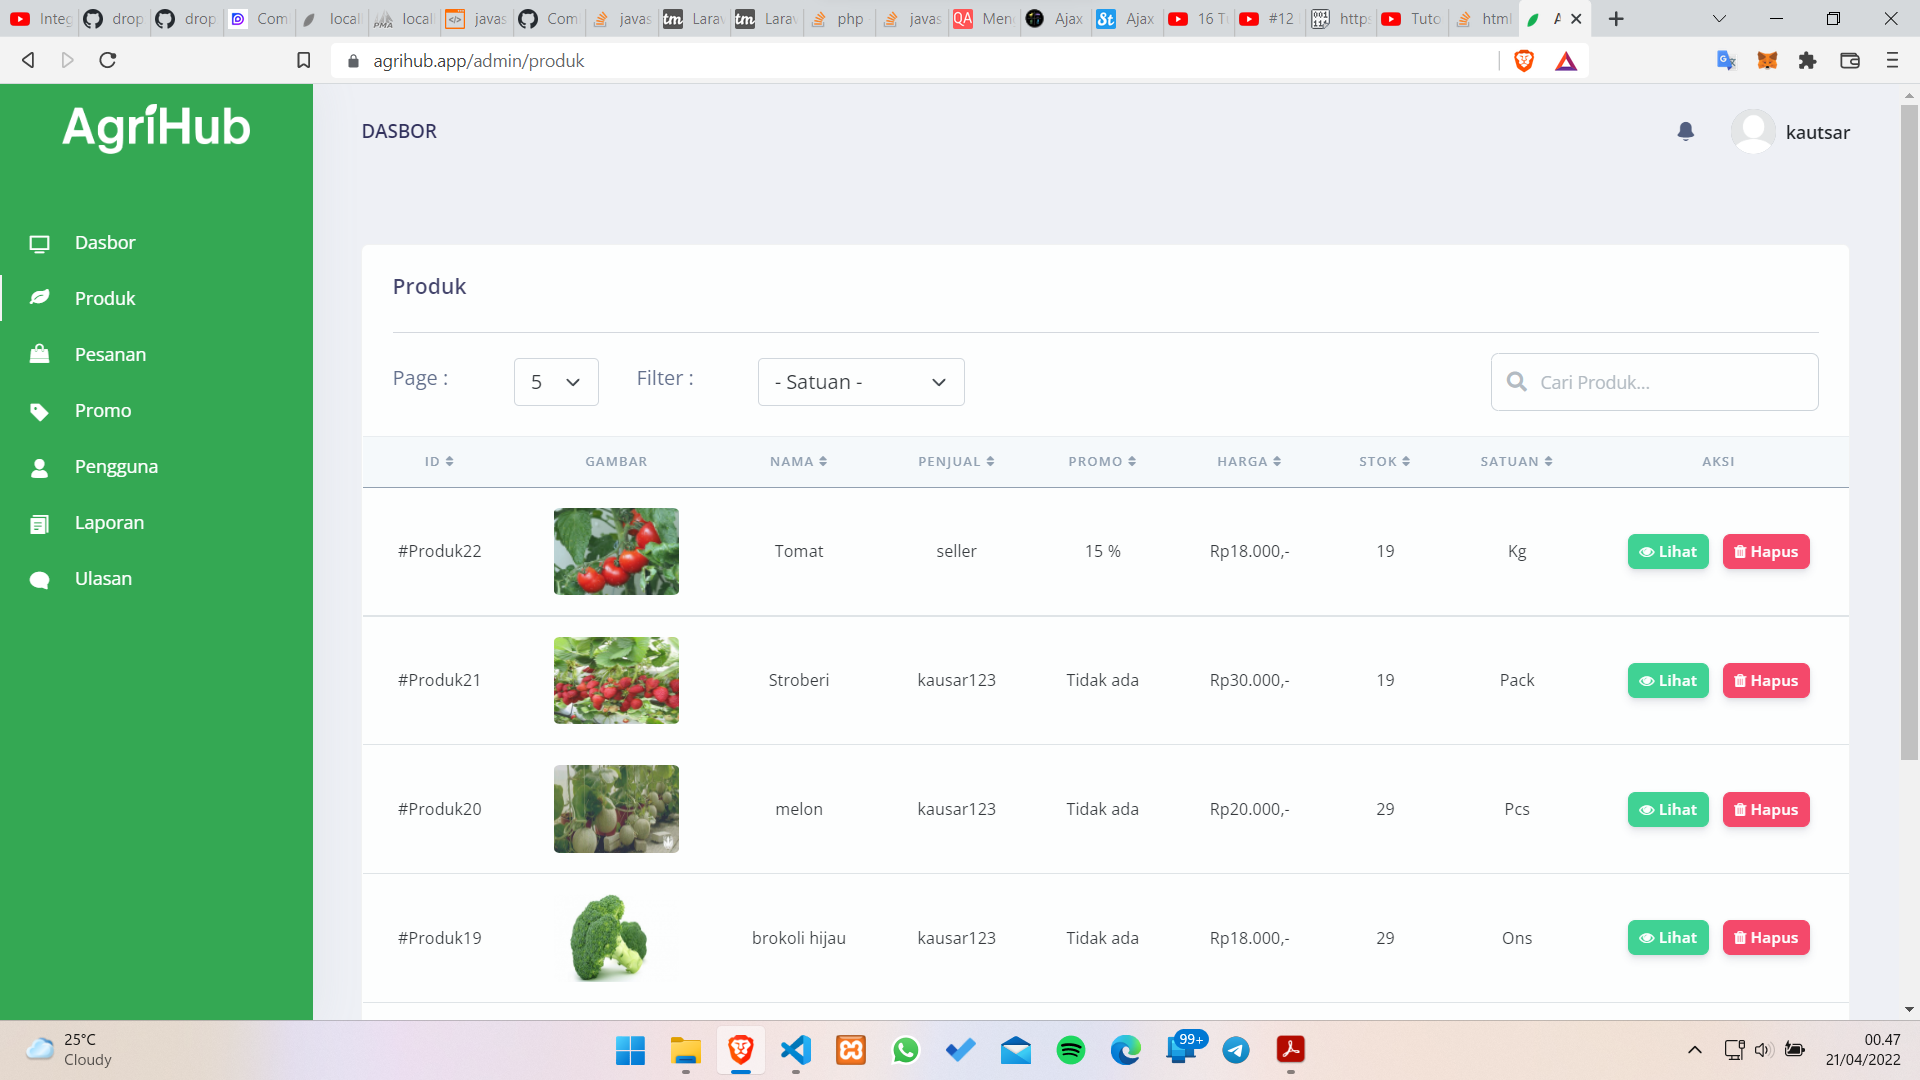
\includegraphics [width = 13cm, height= 7.5cm]{gambar/admin/produk_admin}}
			\caption{Halaman Produk pada sisi Admin}
			\label{produk_admin}
		\end{figure}
		\begin{figure}[H]
			\centering
			{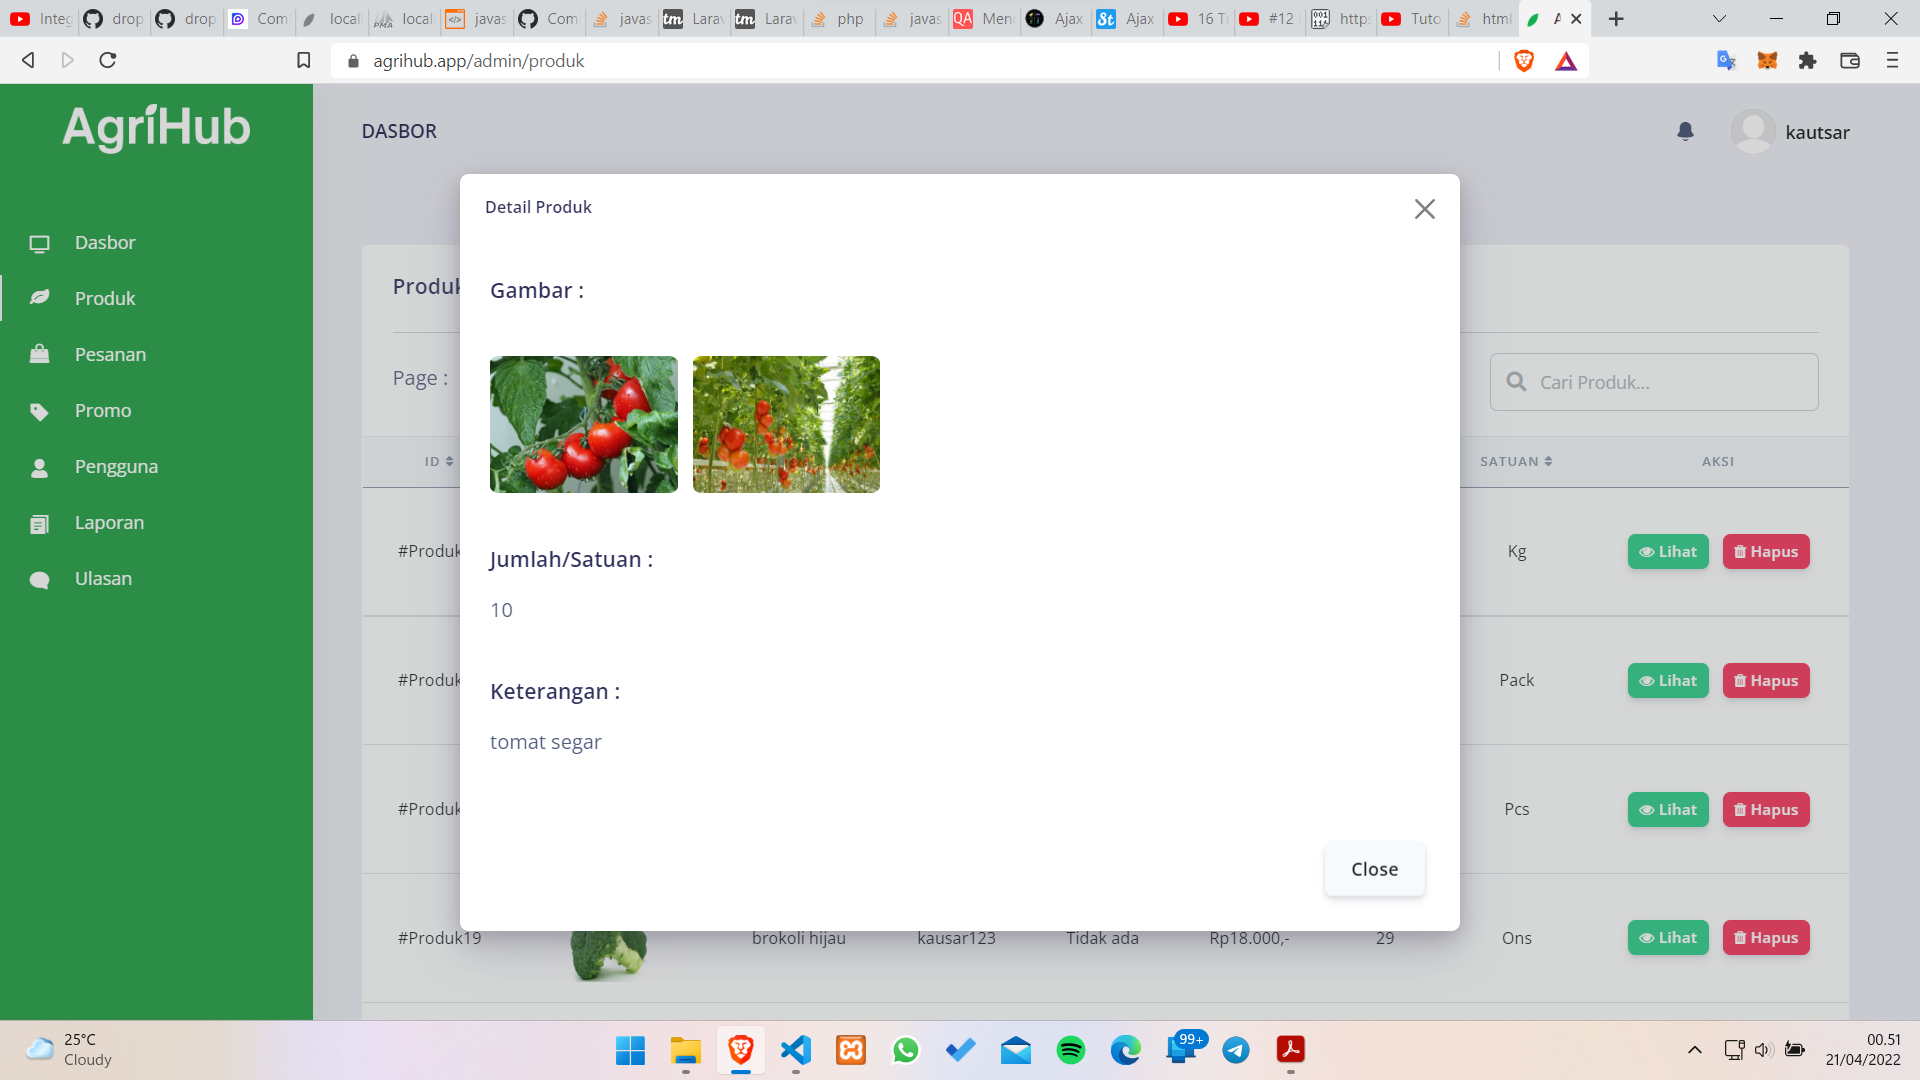
\includegraphics [width = 13cm, height= 7.5cm]{gambar/admin/lihat_produk_admin}}
			\caption{Tampilan Detail Produk}
			\label{lihat_produk_admin}
		\end{figure}

		\item Halaman Pesanan
		\par Pada halaman pesanan admin dapat melihat semua pesanan yang sudah terjadi diaplikasi antara penjual dengan pembeli, dan dapat memfilter datanya berdasarkan status pesanannya. Admin juga dapat melihat detail pesanan dengan menekan tombol Detail serta dapat mengekspor datanya dalam bentuk pdf jika diperlukan dengan menekan tombol \textit{Export} PDF. Halaman pesanan dan tampilan detail serta ekspor pdf pesanan dapat dilihat pada gambar \ref*{pesanan_admin} hingga gambar \ref*{export_pesanan_admin}.
		\begin{figure}[H]
			\centering
			{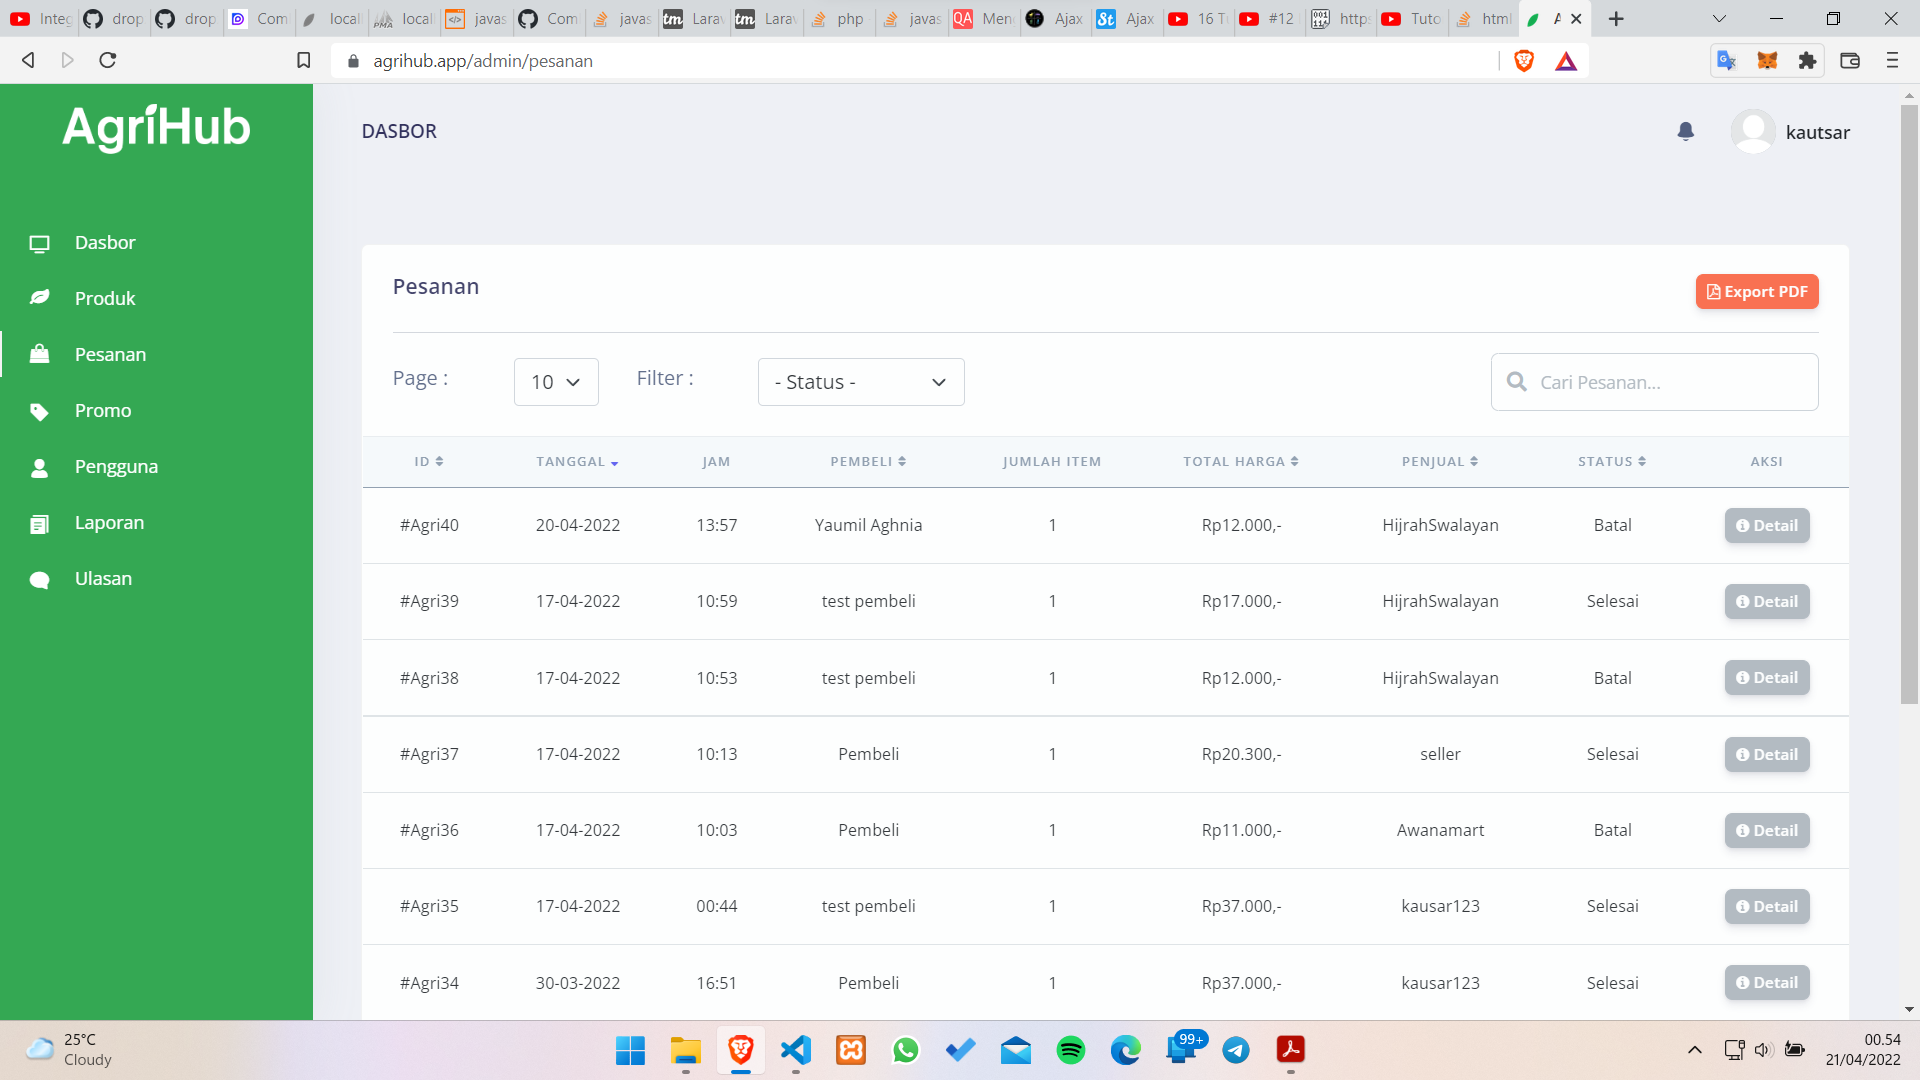
\includegraphics [width = 13cm, height= 7.5cm]{gambar/admin/pesanan_admin}}
			\caption{Halaman Pesanan pada sisi Admin}
			\label{pesanan_admin}
		\end{figure}
		\begin{figure}[H]
			\centering
			{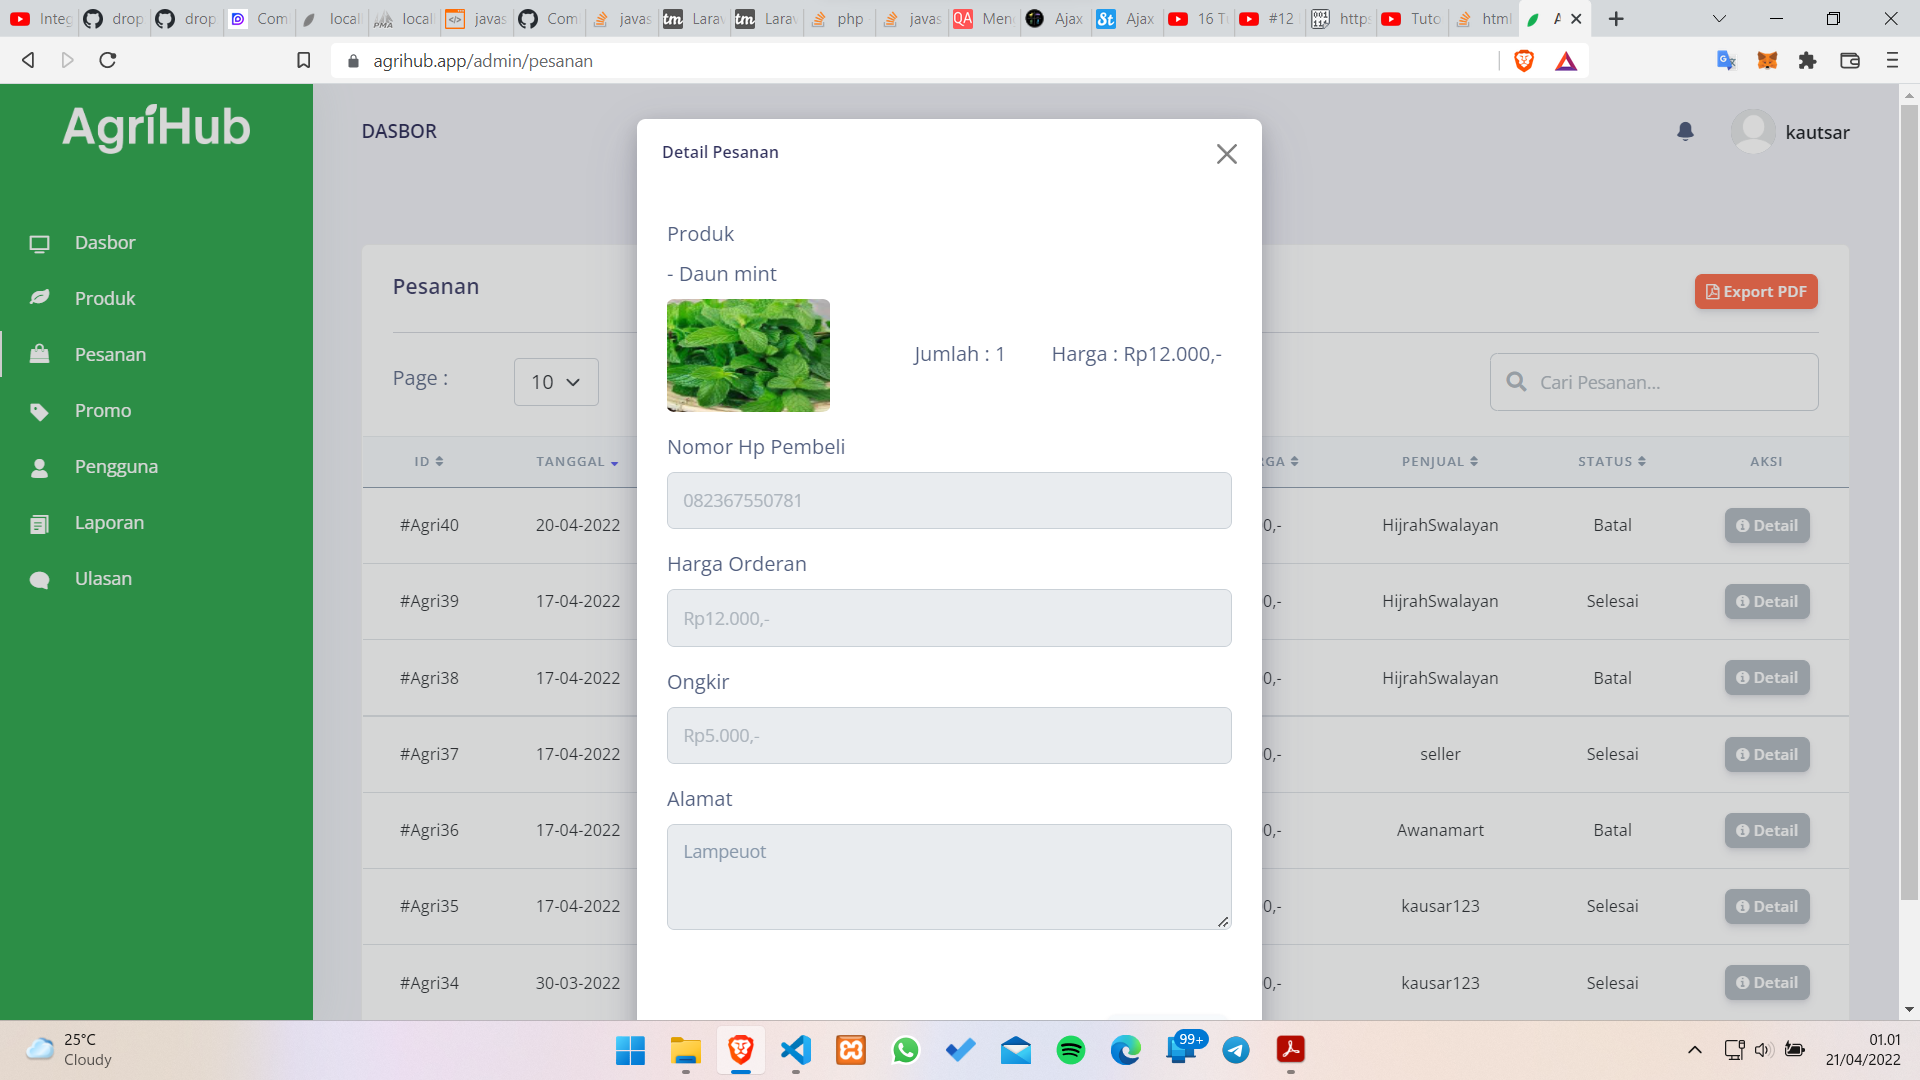
\includegraphics [width = 13cm, height= 7.5cm]{gambar/admin/detail_pesanan}}
			\caption{Tampilan Detail Pesanan}
			\label{detail_pesanan}
		\end{figure}
		\begin{figure}[H]
			\centering
			{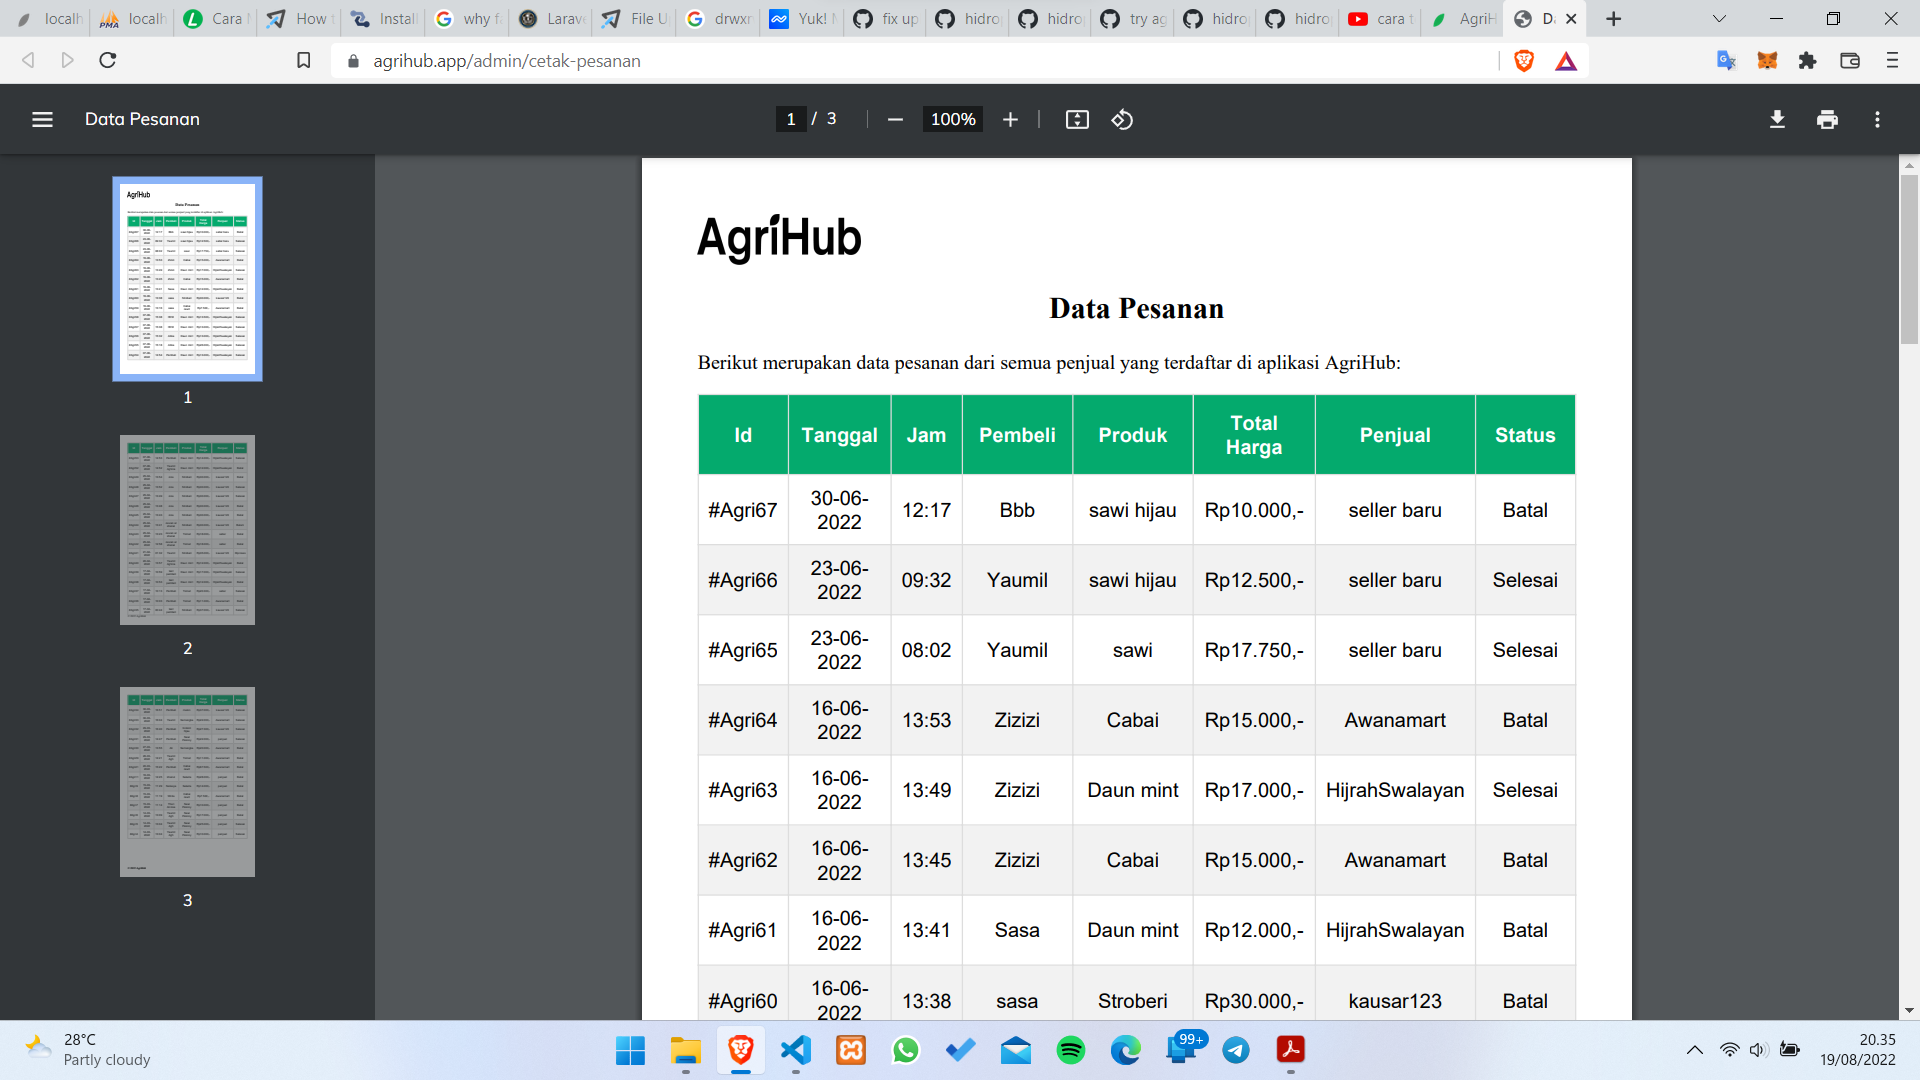
\includegraphics [width = 13cm, height= 7.5cm]{gambar/admin/export_pesanan_admin}}
			\caption{Tampilan Ekspor PDF Pesanan pada sisi Admin}
			\label{export_pesanan_admin}
		\end{figure}

		\item Halaman Promo
		\par Pada halaman ini admin dapat mengelola promo seperti menambahkan promo baru ke dalam aplikasi sehingga nantinya dapat digunakan oleh para penjual, dan dapat juga mengubah data promo yang sudah ada atau menghapusnya. Halaman promo dan tampilan tambah serta ubah promo dapat dilihat pada gambar \ref*{promo} hingga gambar \ref*{ubah_promo}.
		\begin{figure}[H]
			\centering
			{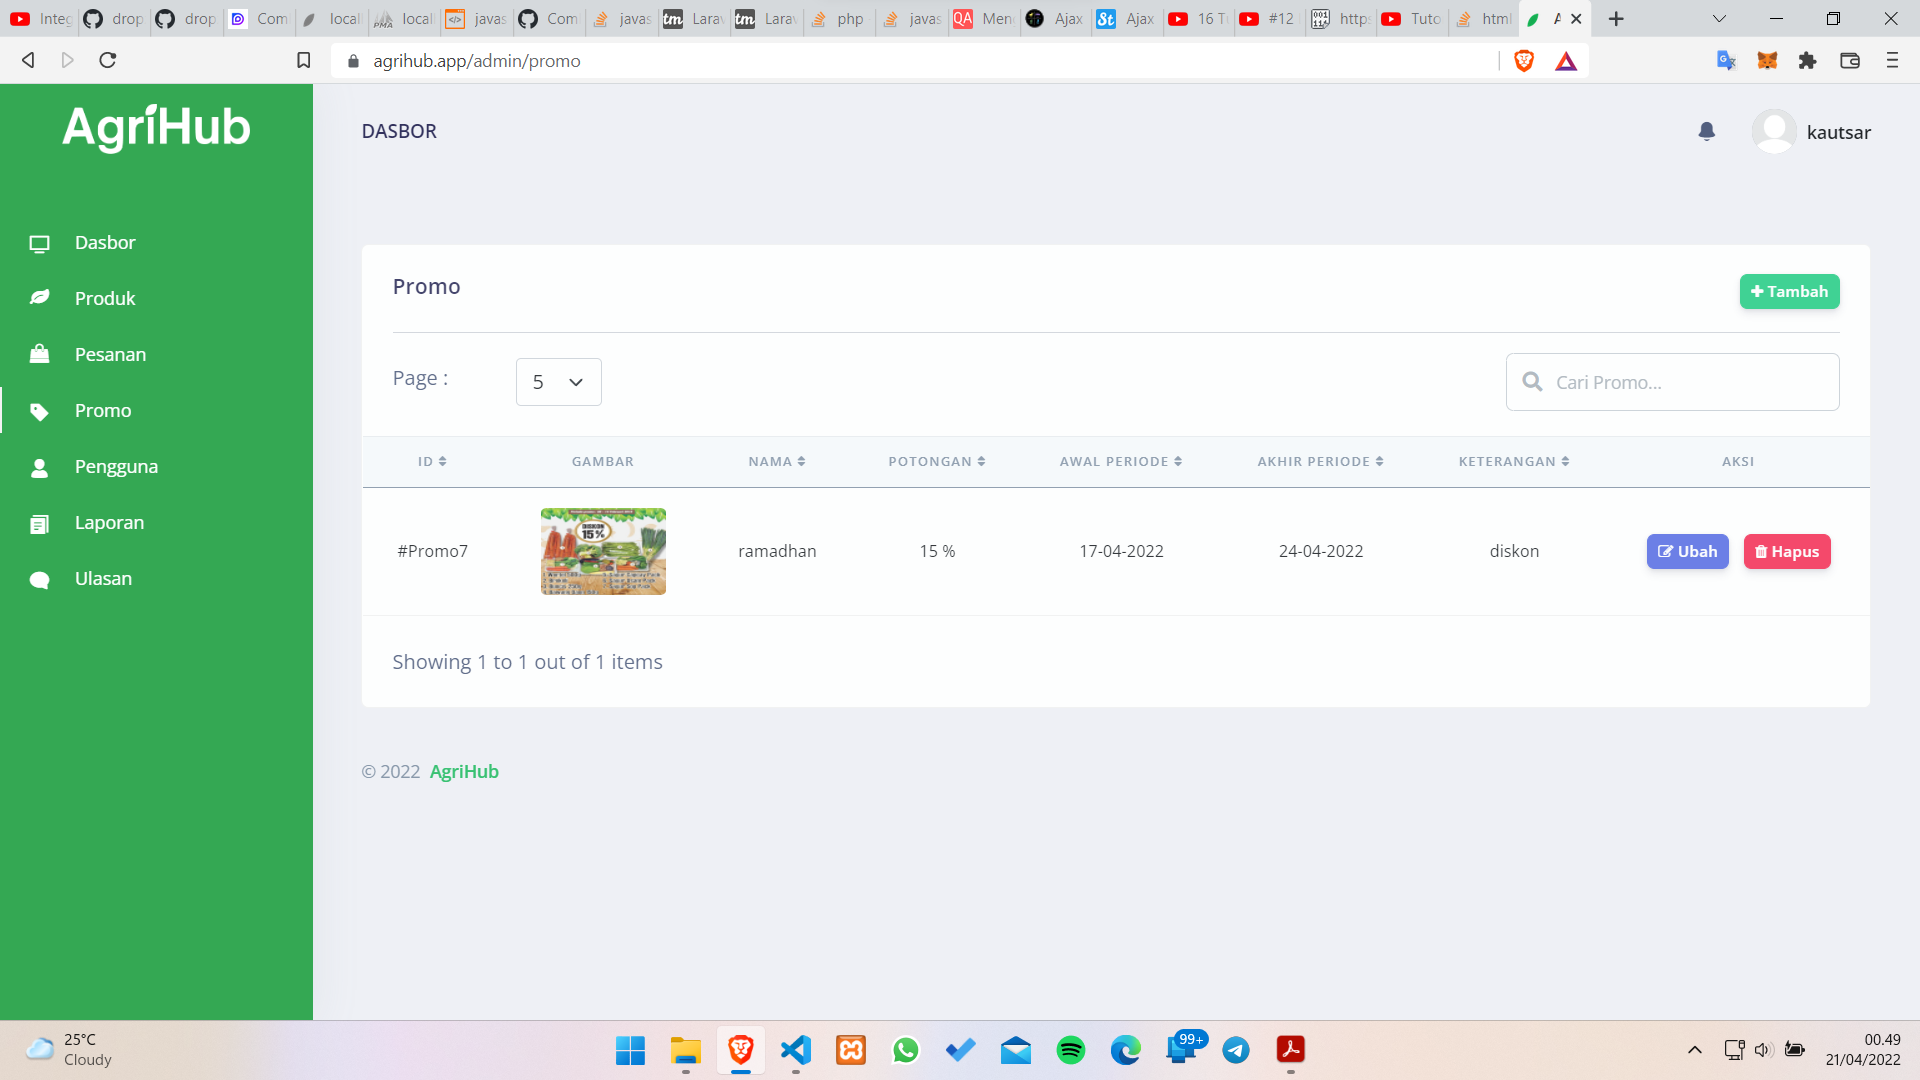
\includegraphics [width = 13cm, height= 7.5cm]{gambar/admin/promo}}
			\caption{Halaman Promo}
			\label{promo}
		\end{figure}
		\begin{figure}[H]
			\centering
			{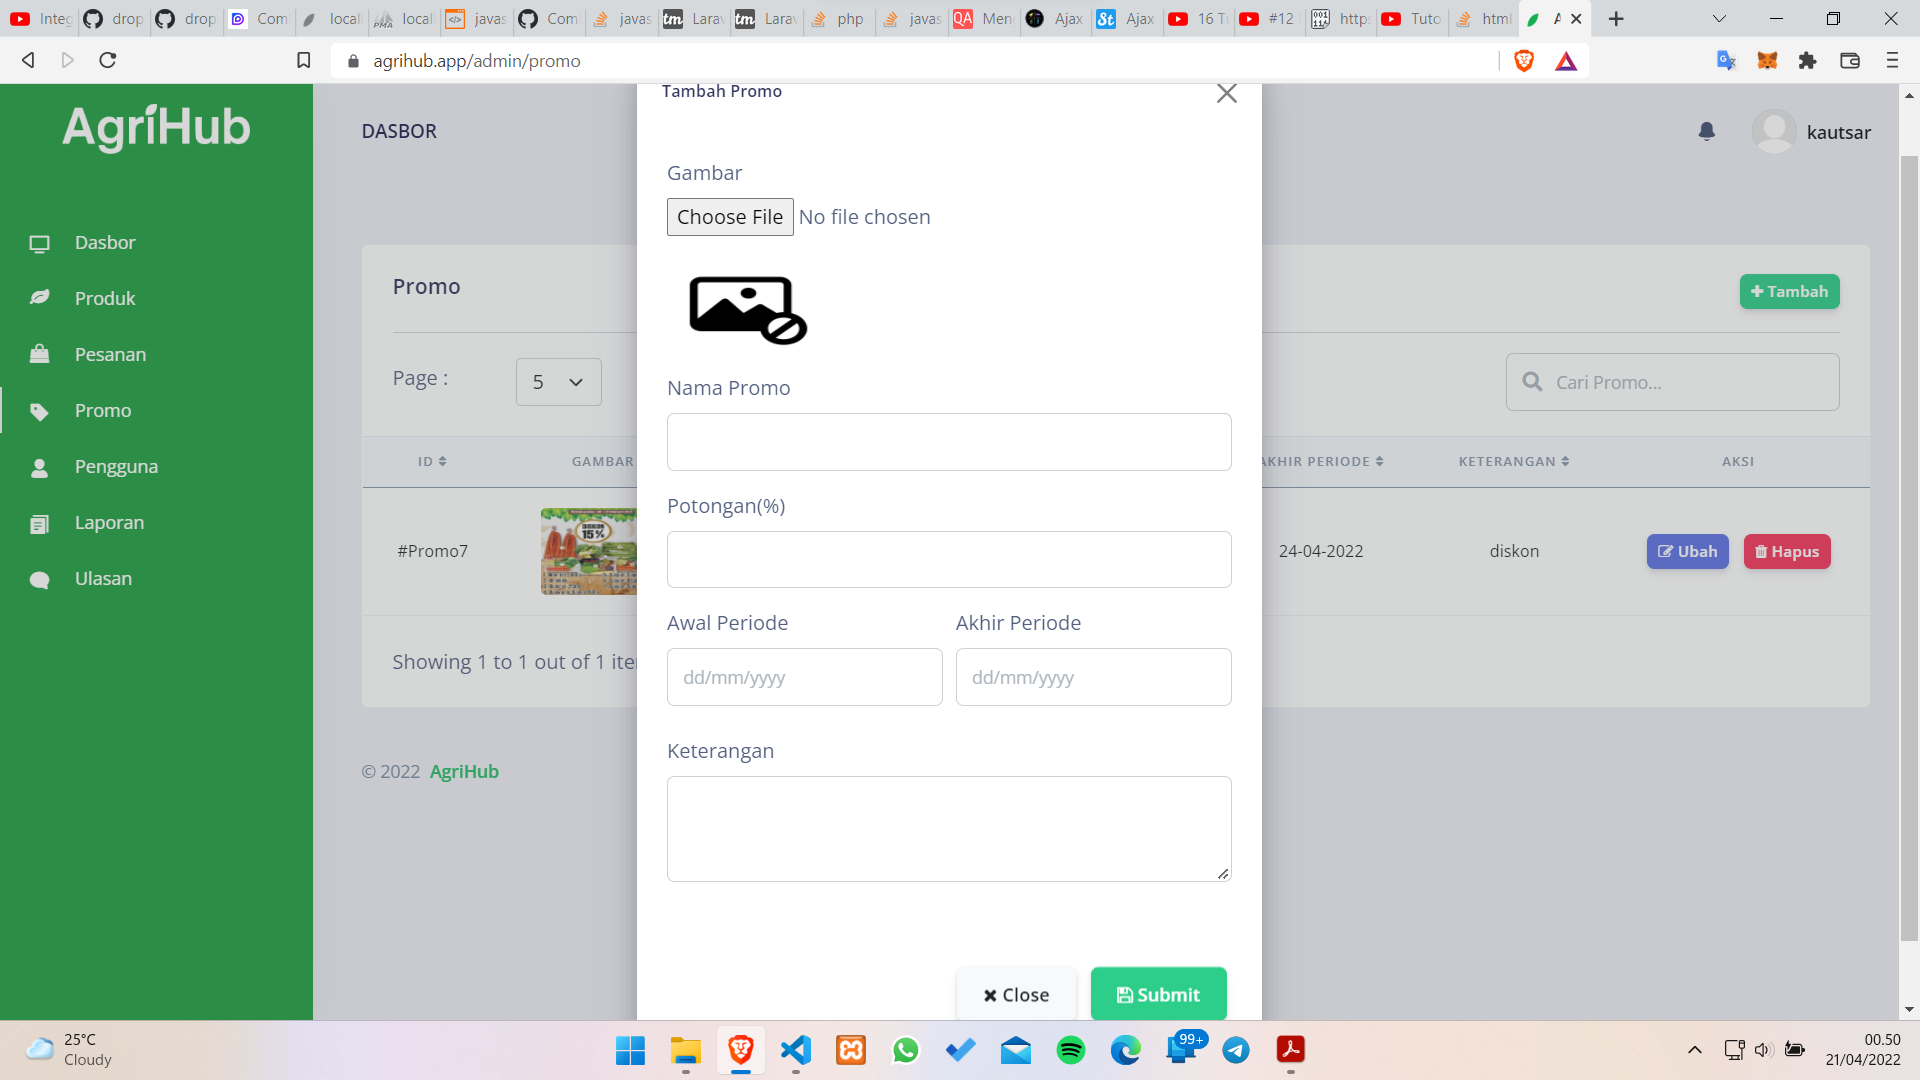
\includegraphics [width = 13cm, height= 7.5cm]{gambar/admin/tambah_promo}}
			\caption{Tampilan Tambah Promo}
			\label{tambah_promo}
		\end{figure}
		\begin{figure}[H]
			\centering
			{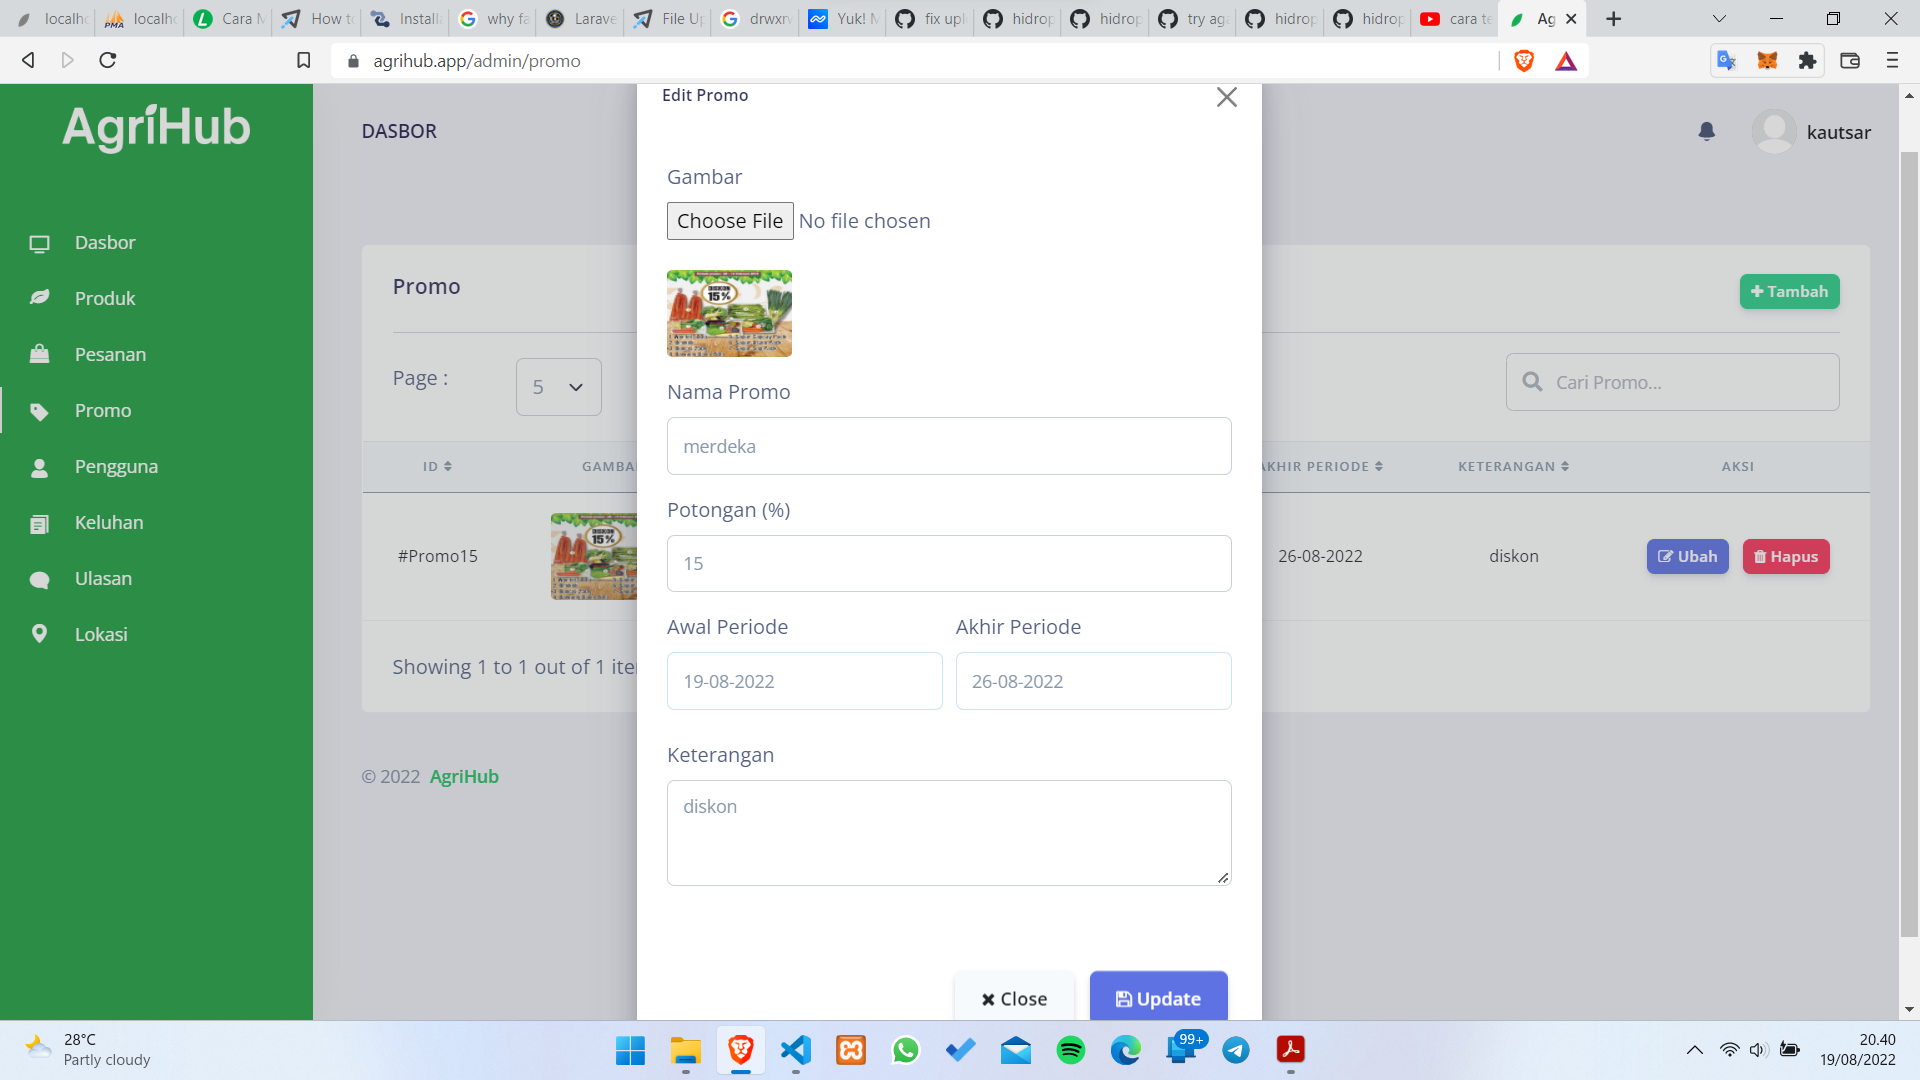
\includegraphics [width = 13cm, height= 7.5cm]{gambar/admin/ubah_promo}}
			\caption{Tampilan Ubah Promo}
			\label{ubah_promo}
		\end{figure}

		\item Halaman Pengguna
		\par Pada halaman pengguna ini admin data melihat semua data pengguna yang sudah terdaftar diaplikasi AgriHub ini baik itu admin, penjual maupun pembeli, serta dapat memblokir penjual atau pembeli yang melanggar. Juga dapat menambahkan akun penjual baru dengan menekan tombol tambah penjual dan mengisi data penjual. Halaman pengguna dan tampilan tambah akun penjual dapat dilihat pada gambar \ref*{pengguna}-\ref*{tambah_pengguna}.
		\begin{figure}[H]
			\centering
			{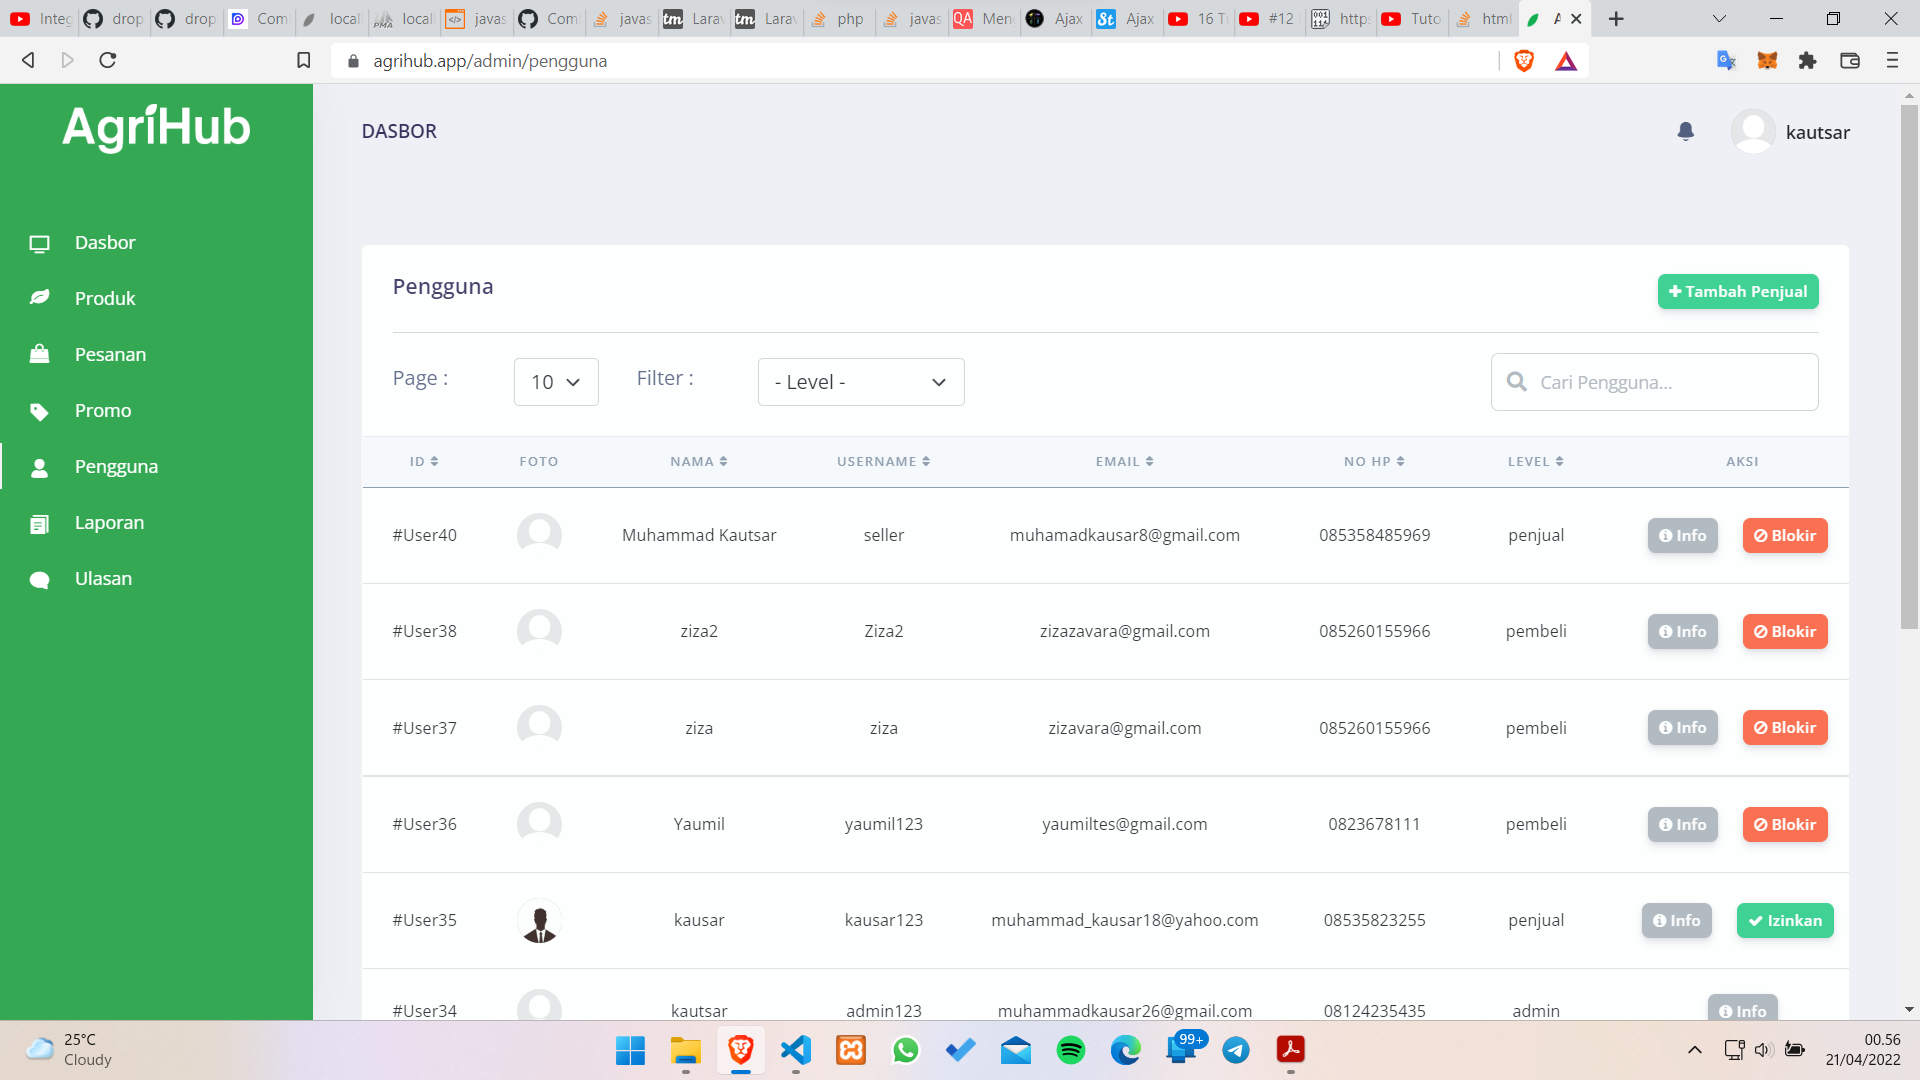
\includegraphics [width = 13cm, height= 7.5cm]{gambar/admin/pengguna}}
			\caption{Halaman Pengguna}
			\label{pengguna}
		\end{figure}
		\begin{figure}[H]
			\centering
			{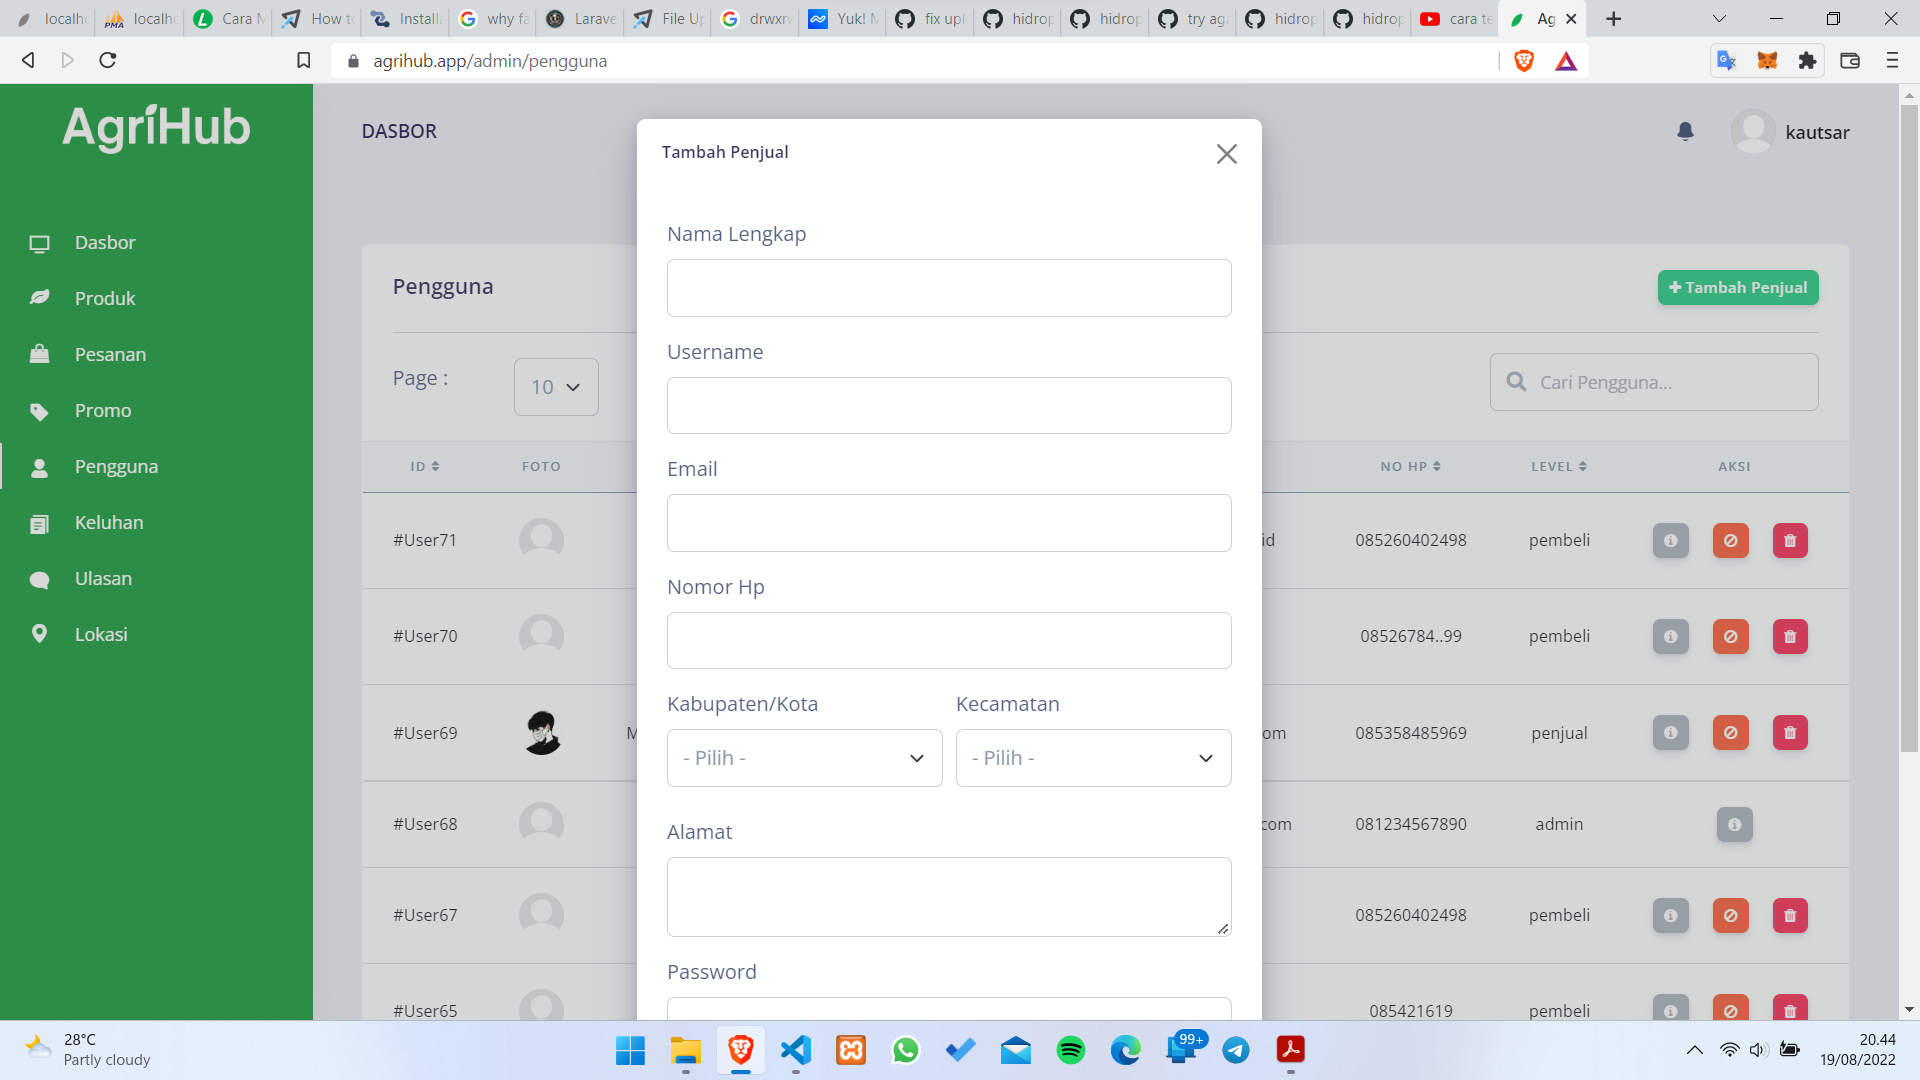
\includegraphics [width = 13cm, height= 7.5cm]{gambar/admin/tambah_pengguna}}
			\caption{Tampilan Tambah Akun Penjual}
			\label{tambah_pengguna}
		\end{figure}

		\item Halaman Laporan
		\par Pada halaman ini admin dapat melihat data laporan yang masuk dari para pembeli terhadap penjual seperti id, tanggal, isi laporan, nama pelapor dan nama penjual yang dilaporkan. Setelah mendapat laporan dari pembeli, admin dapat mengambil tindakan pemblokiran pada akun penjual tersebut melalui halaman pengguna. Halaman laporan dapat dilihat pada gambar \ref*{laporan}.
		\begin{figure}[H]
			\centering
			{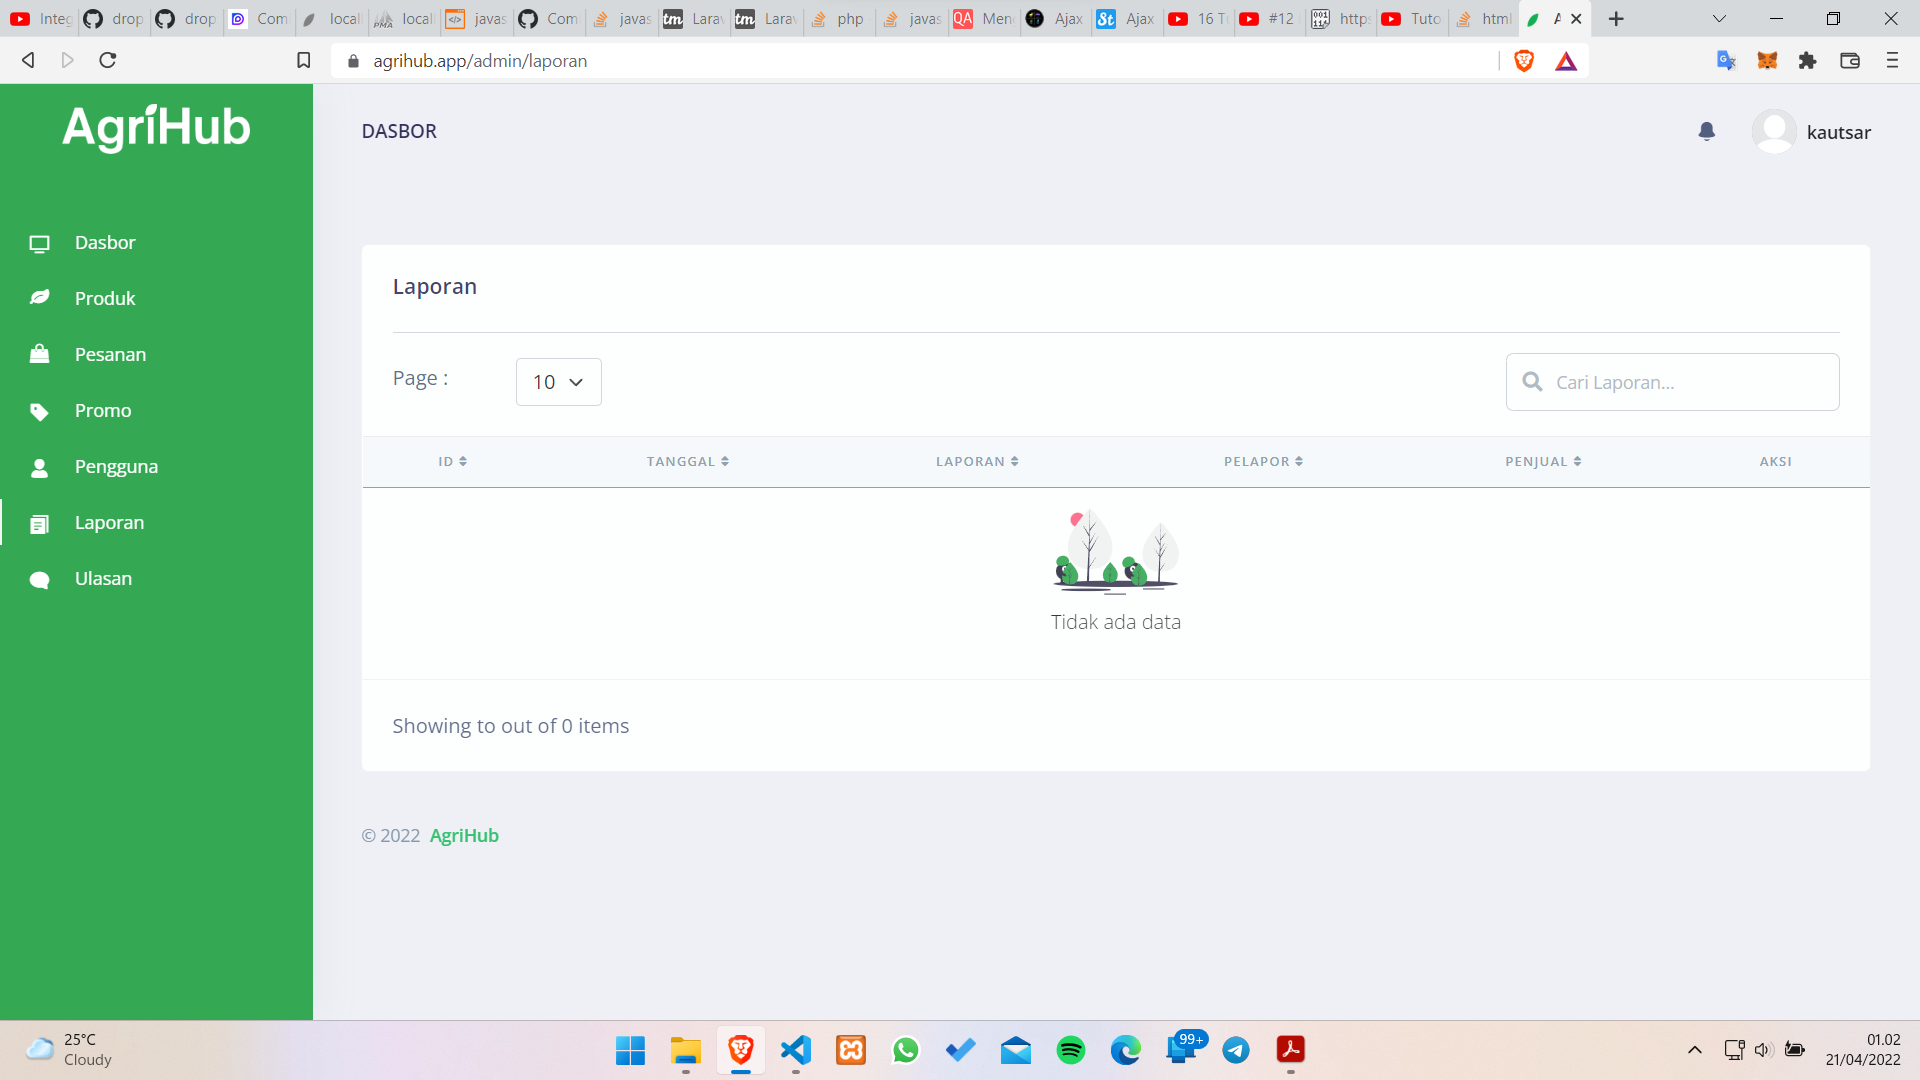
\includegraphics [width = 13cm, height= 7.5cm]{gambar/admin/laporan}}
			\caption{Halaman Laporan}
			\label{laporan}
		\end{figure}

		\item Halaman Ulasan
		\par Halaman ulasan berisi semua ulasan yang sudah diberikan oleh para pembeli terhadap produk yang dia beli dari penjual. Admin dapat memfilter ulasannya berdasarkan \textit{rating} bintang yang diberikan oleh pembeli dan dapat juga menghapus ulasan pembeli jika dianggap mengandung kata tidak pantas. Halaman ulasan dapat dilihat pada gambar \ref*{ulasan_admin}.
		\begin{figure}[H]
			\centering
			{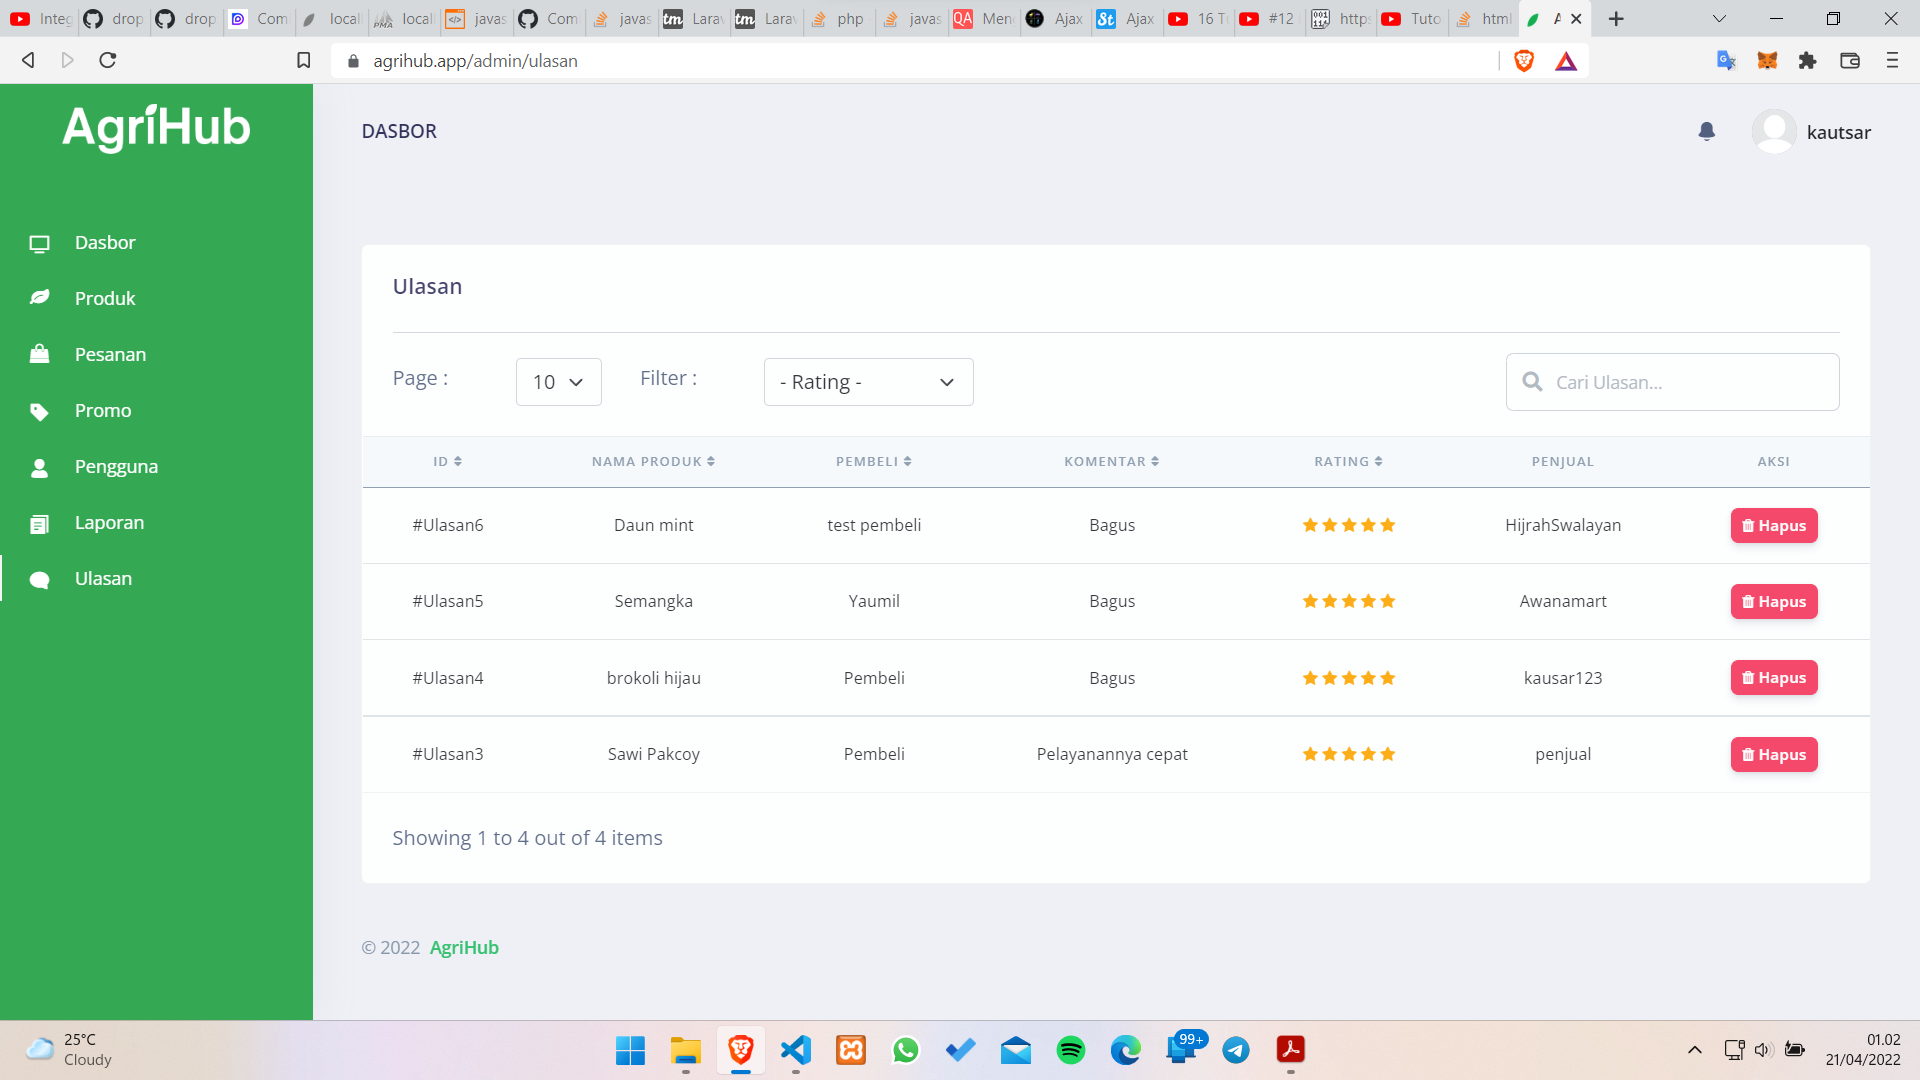
\includegraphics [width = 13cm, height= 7.5cm]{gambar/admin/ulasan_admin}}
			\caption{Halaman Ulasan pada sisi Admin}
			\label{ulasan_admin}
		\end{figure}
	\end{enumerate}

	\newpage
	\item Antarmuka Aplikasi Bagian Penjual
	\par Antarmuka aplikasi pada bagian penjual pada dasarnya hampir sama seperti antarmuka pada bagian admin hanya saja ada beberapa halaman dan menunya yang berbeda. Halaman aplikasi pada bagian penjual sebagai berikut :

	\begin{enumerate}[a.]
		\item Halaman Informasi
		\par Halaman informasi menampilkan informasi mengenai tata cara mendaftar sebagai penjual diaplikasi AgriHub ini. Penjual dapat mengakses halaman informasi ini dengan menklik \textit{tab} informasi yang ada dipojok kanan atas pada halaman utama. Halaman informasi dapat dilihat pada gambar \ref*{informasi}.
		\begin{figure}[H]
			\centering
			{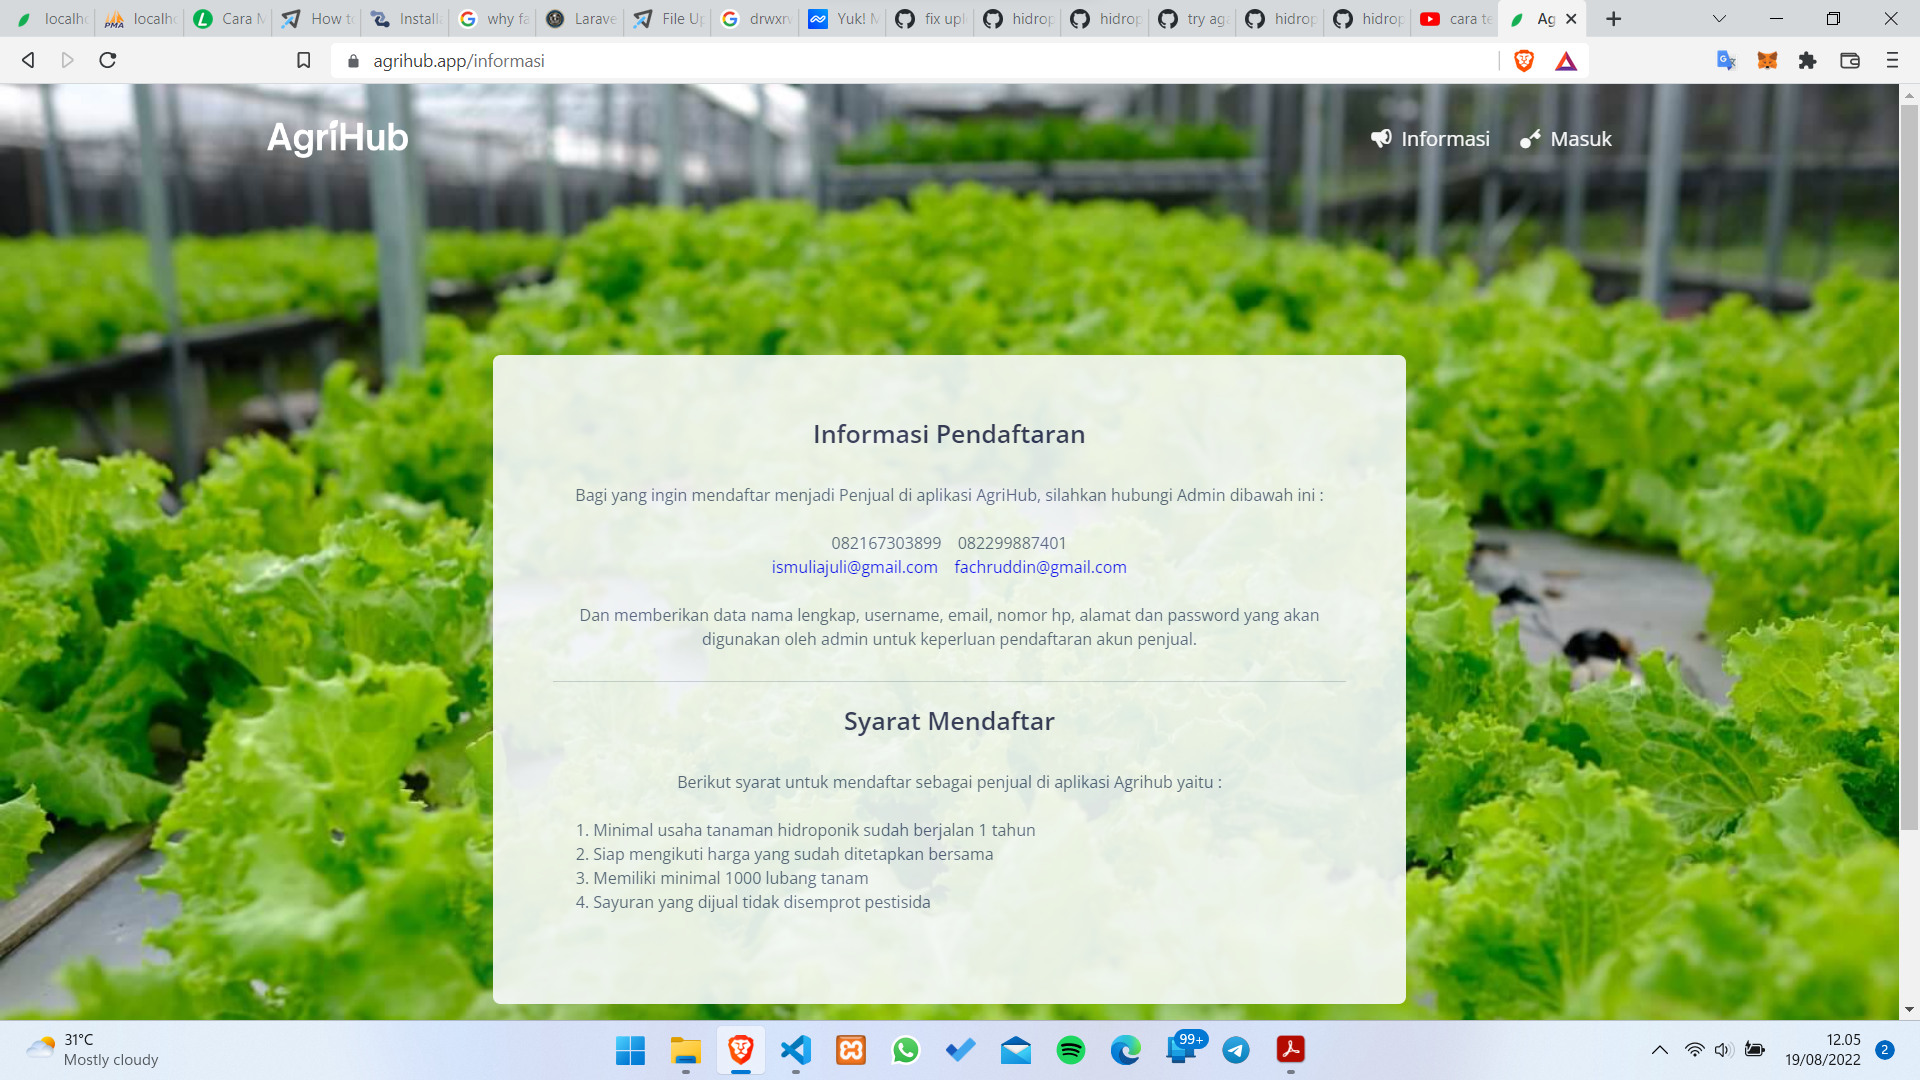
\includegraphics [width = 13cm, height= 7.5cm]{gambar/informasi}}
			\caption{Halaman Informasi}
			\label{informasi}
		\end{figure}

		\item Halaman Masuk
		\par Halaman masuk (\textit{login}) penjual sama seperti pada bagian admin, hanya saja ada sedikit perbedaan ketika akun penjual diblokir oleh admin karna melakukan kesalahan. Maka akun penjual tersebut tidak bisa masuk ke dalam aplikasi. Supaya akunnya penjual dapat digunakan kembali bisa menghubungi admin terlebih dahulu. Tampilan diblokir dapat dilihat pada gambar \ref*{diblokir}.
		\begin{figure}[H]
			\centering
			{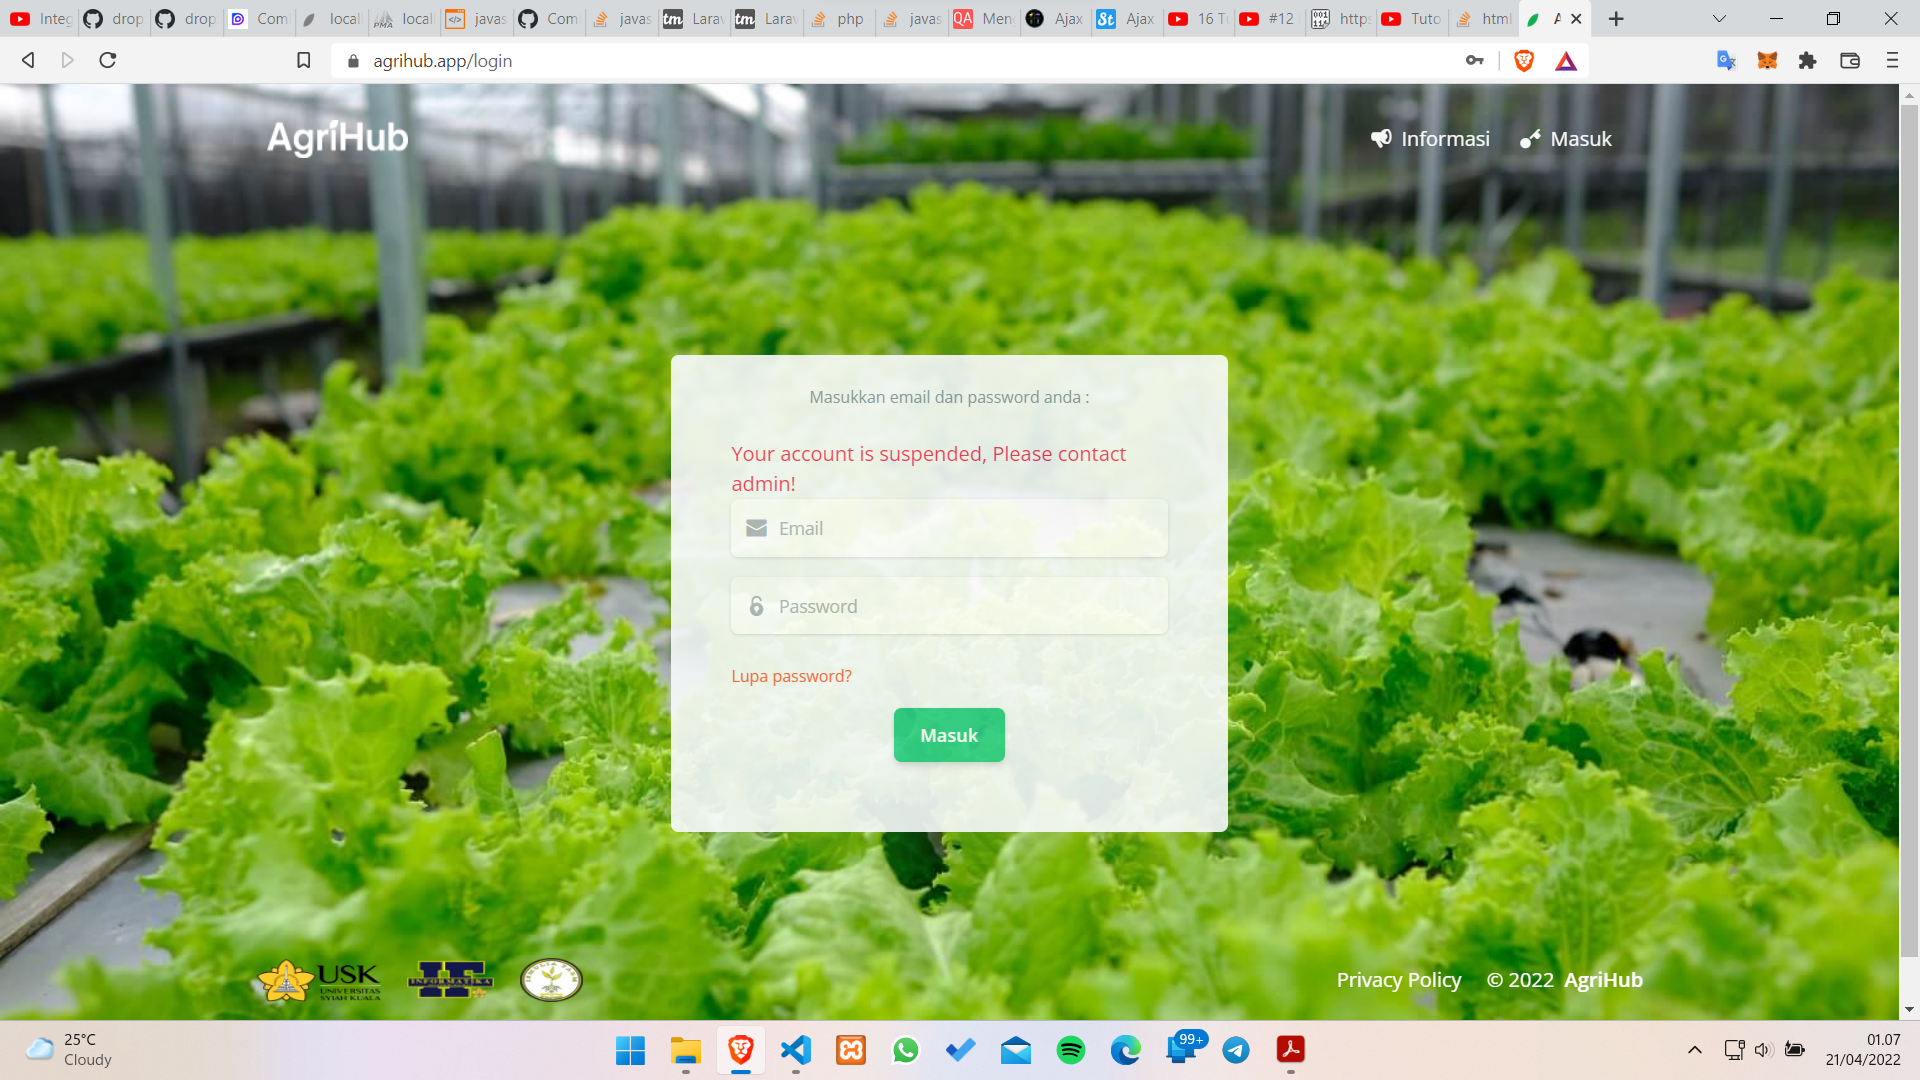
\includegraphics [width = 13cm, height= 7.5cm]{gambar/diblokir}}
			\caption{Tampilan Diblokir}
			\label{diblokir}
		\end{figure}

		\item Halaman Lupa \textit{Password}
		\par Apabila penjual lupa \textit{password} akunnya, maka dapat menklik tulisan lupa \textit{password} yang ada pada halaman masuk kemudian akan diarahkan ke halaman lupa \textit{password}. Pada halaman ini penjual dapat mengisikan emailnya, supaya nanti dikirimkan \textit{email reset password} ke alamat \textit{email} terdaftar untuk mengubah \textit{password}nya. Halaman lupa \textit{password} dapat dilihat pada gambar \ref*{lupa_password}.
		\begin{figure}[H]
			\centering
			{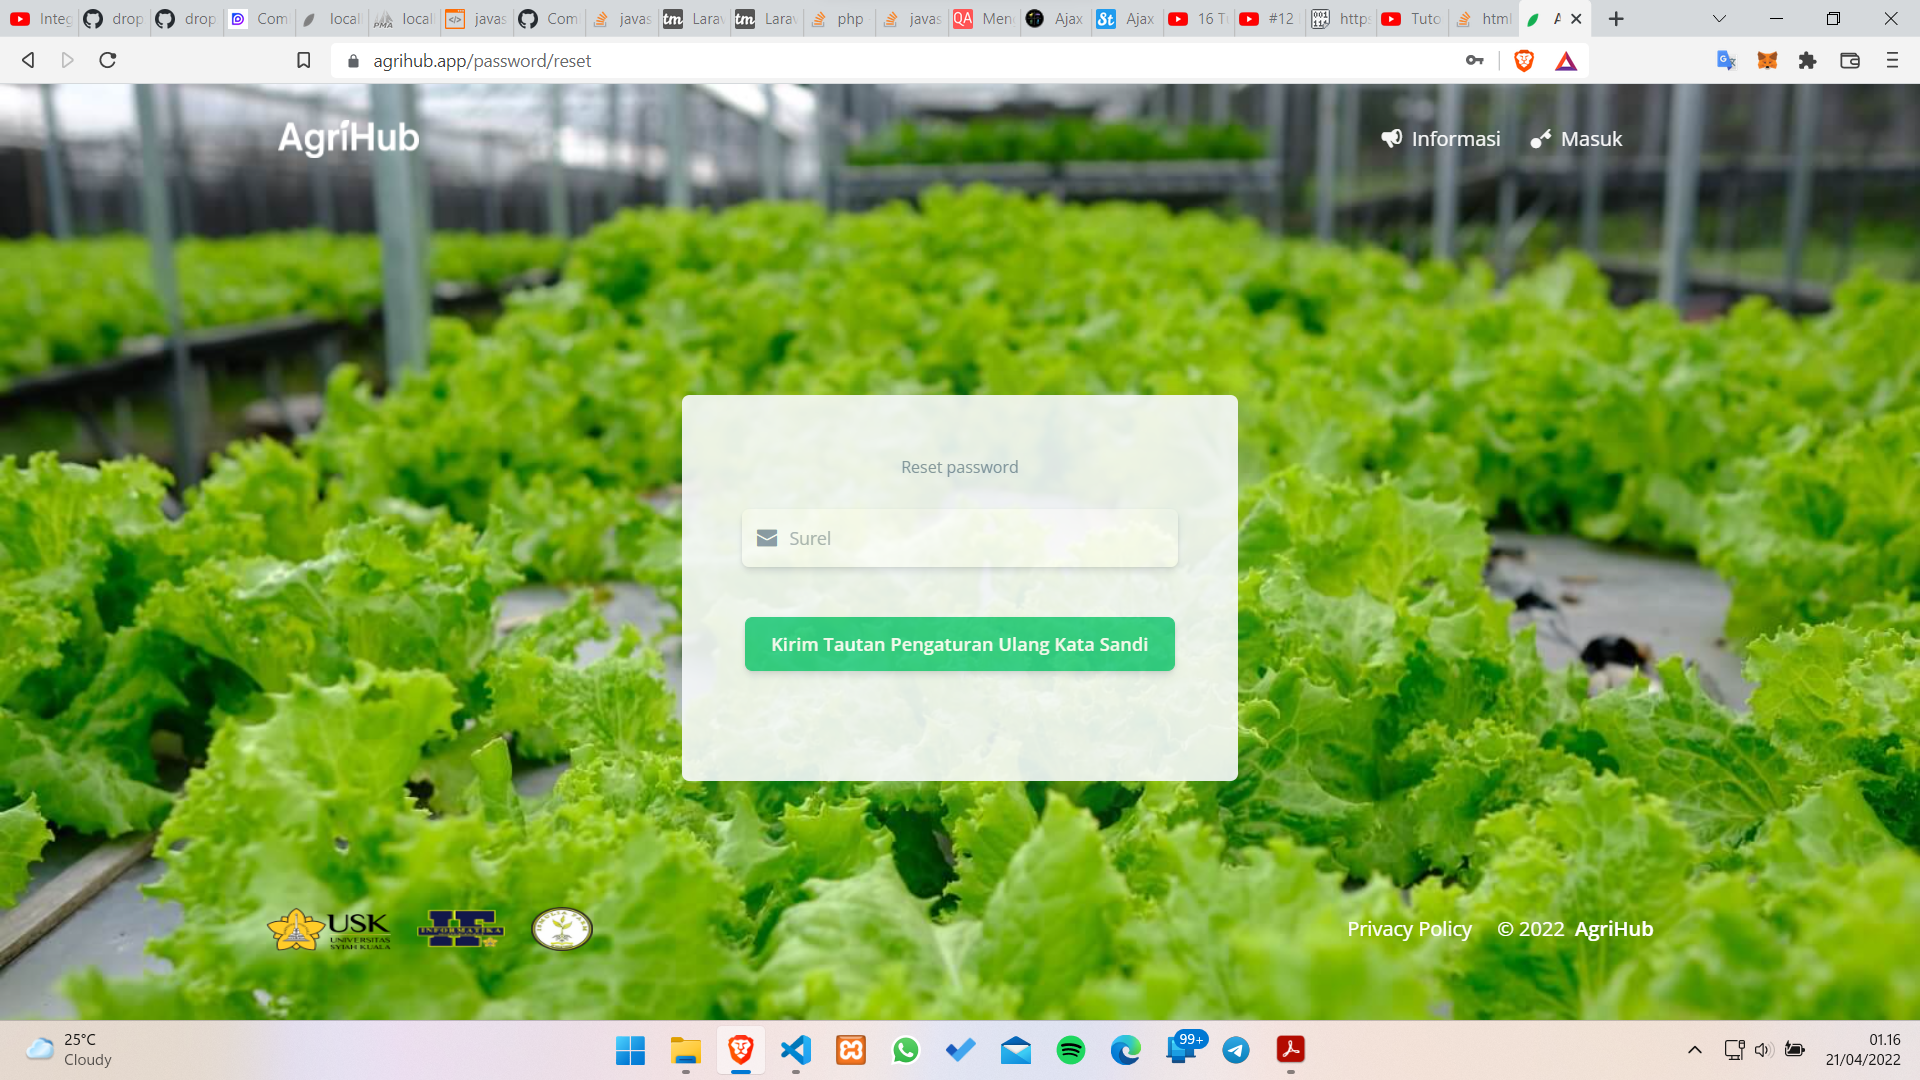
\includegraphics [width = 13cm, height= 7.5cm]{gambar/lupa_password}}
			\caption{Halaman Lupa \textit{Password}}
			\label{lupa_password}
		\end{figure}

		\newpage
		\item Halaman Dasbor
		\par Apabila penjual telah berhasil masuk ke dalam aplikasi, maka akan tampil halaman dasbor yang berisi keterangan mengenai jumlah order baru yang masuk, lagi diproses, dikirim, yang sudah selesai dan jumlah order yang batal, serta jumlah ulasan yang sudah diberikan oleh pembeli. Juga ada grafik jumlah pendapatan perbulan yang sudah diperoleh oleh penjual beserta dengan jumlah pesanan yang selesai dan batal perbulannya selama 6 bulan terakhir. Halaman dasbor penjual dapat dilihat pada gambar \ref*{dashboard_penjual}.
		\begin{figure}[H]
			\centering
			{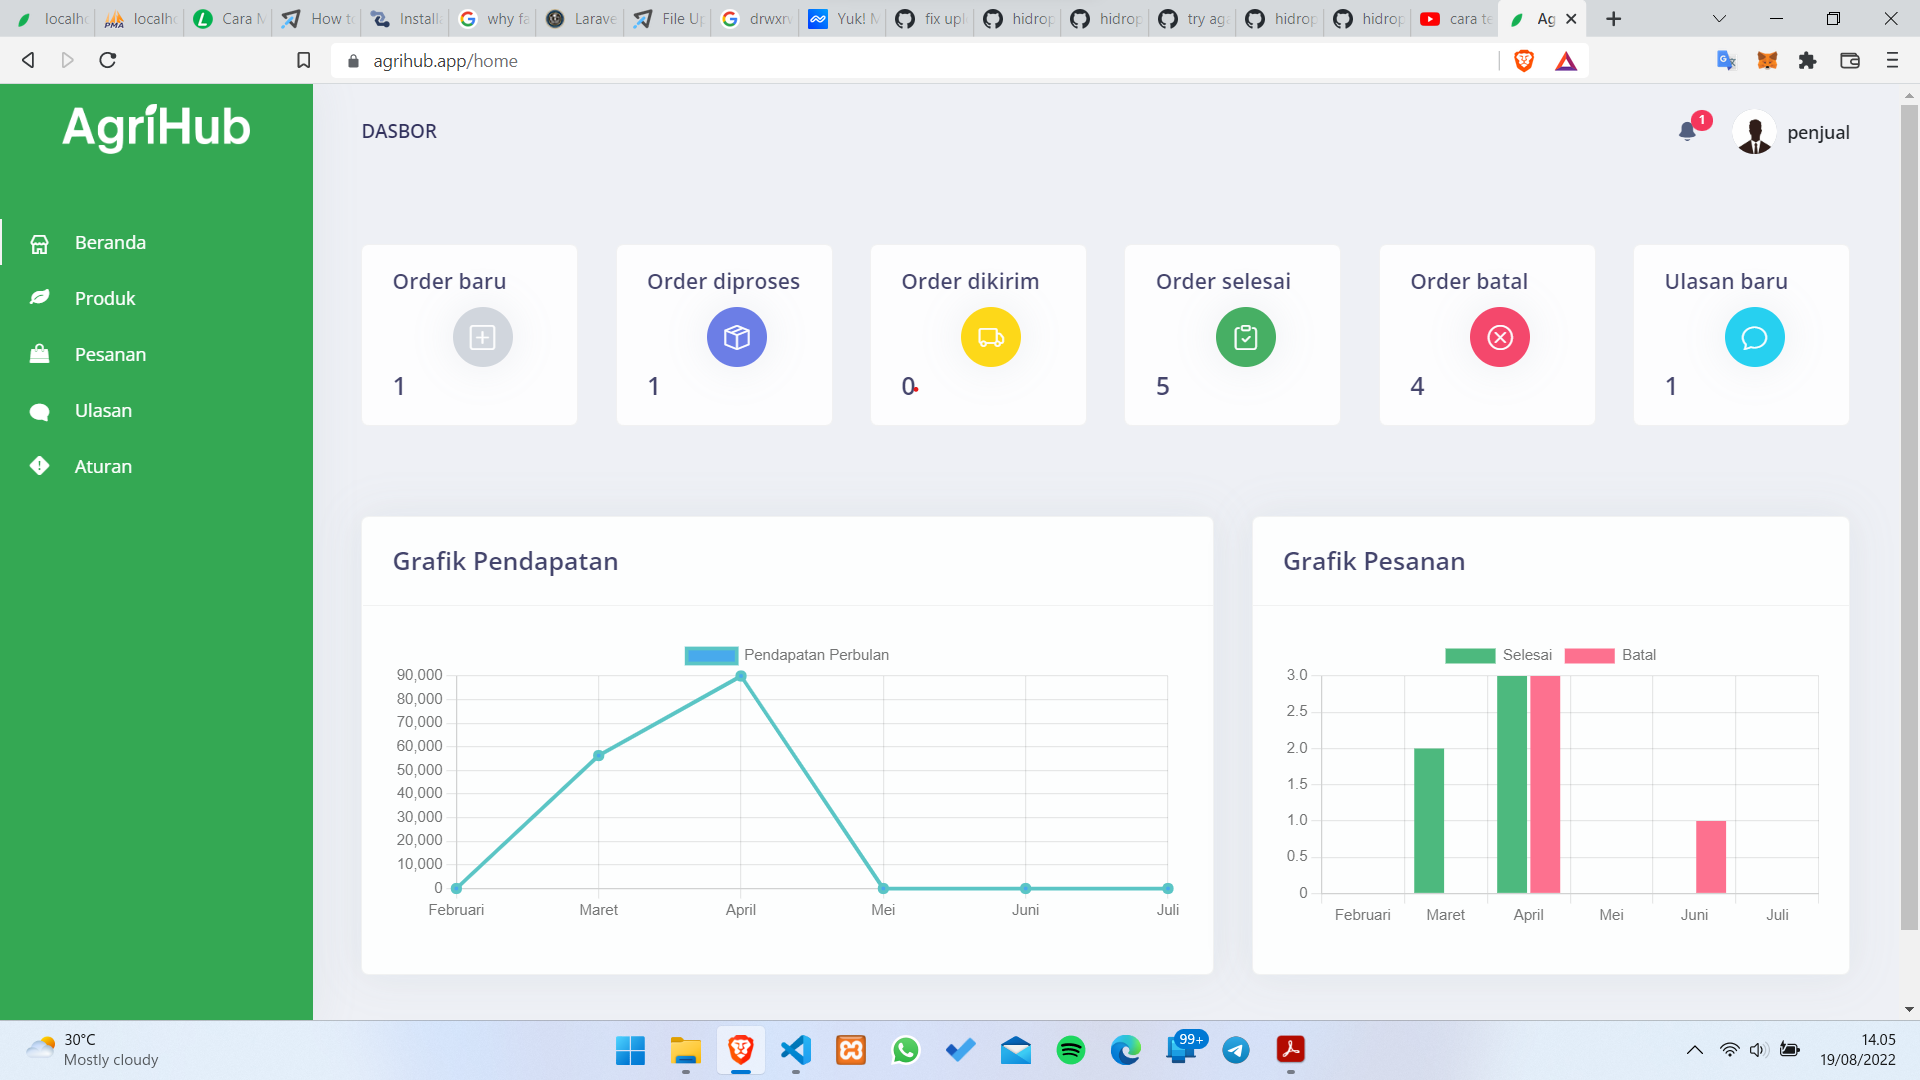
\includegraphics [width = 13cm, height= 7.5cm]{gambar/penjual/dashboard_penjual}}
			\caption{Halaman Dasbor pada sisi Penjual}
			\label{dashboard_penjual}
		\end{figure}

		\item Halaman Produk
		\par Pada halaman produk ini penjual dapat mengelola produknya yang ingin dijual seperti menambahkan produk baru, mengubah data produk yang sudah ada atau menghapus produk yang tidak ingin dijual lagi. Apabila penjual ingin menambahkan produk baru dapat melakukannya dengan menekan tombol tambah, maka akan muncul tampilan tambah produk dan mengisi data-data produk seperti gambar, nama, harga, stok, satuan, jumlah per satuan dan keterangan. Ada juga kolom promo yang bersifat opsional yang bisa dipakai oleh penjual jika admin menyediakan promo. Jika penjual ingin mengubah data produk dapat menekan tombol ubah yang akan diarahkan ke halaman ubah produk dan jika ingin menghapus produk dapat menekan tombol hapus. Halaman produk dan tampilan tambah produk dapat dilihat pada gambar \ref*{produk_penjual} dan gambar \ref*{tambah_produk}.
		\begin{figure}[H]
			\centering
			{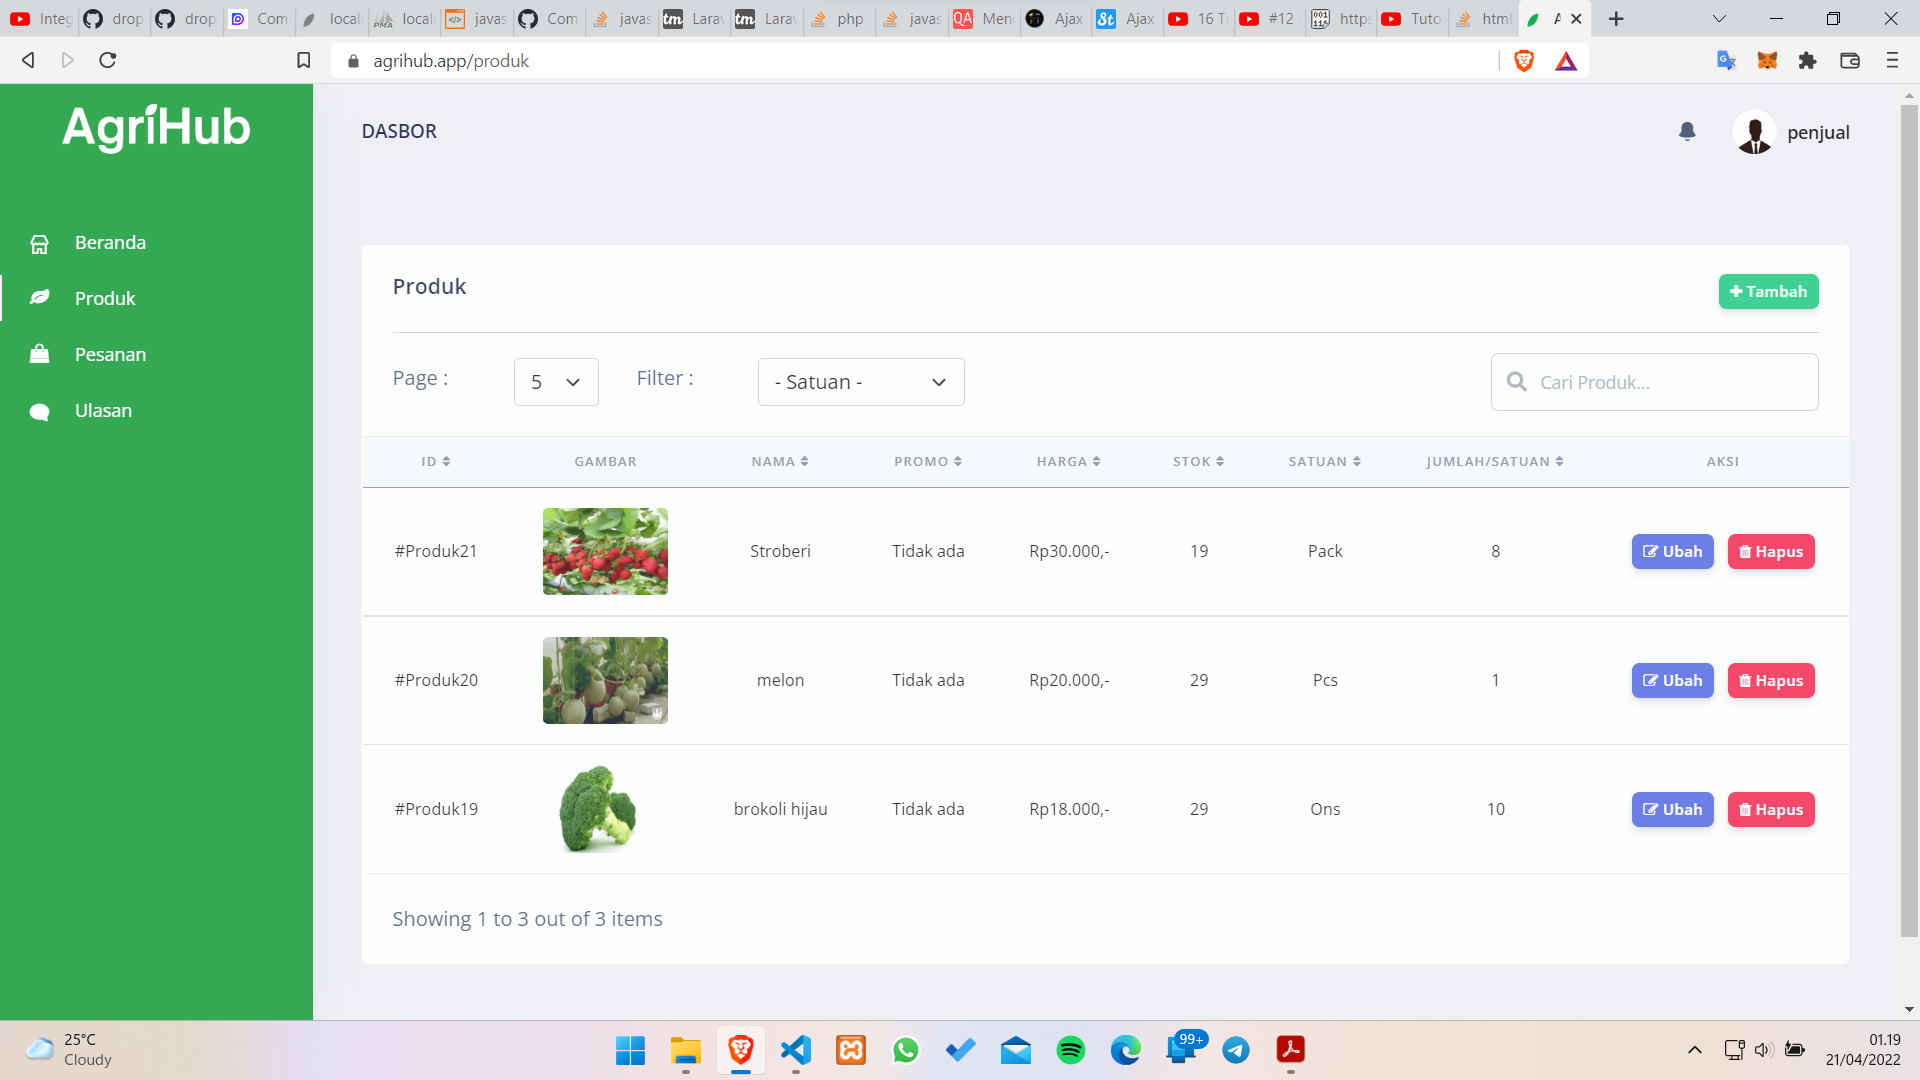
\includegraphics [width = 13cm, height= 7.5cm]{gambar/penjual/produk_penjual}}
			\caption{Halaman Produk pada sisi Penjual}
			\label{produk_penjual}
		\end{figure}
		\begin{figure}[H]
			\centering
			{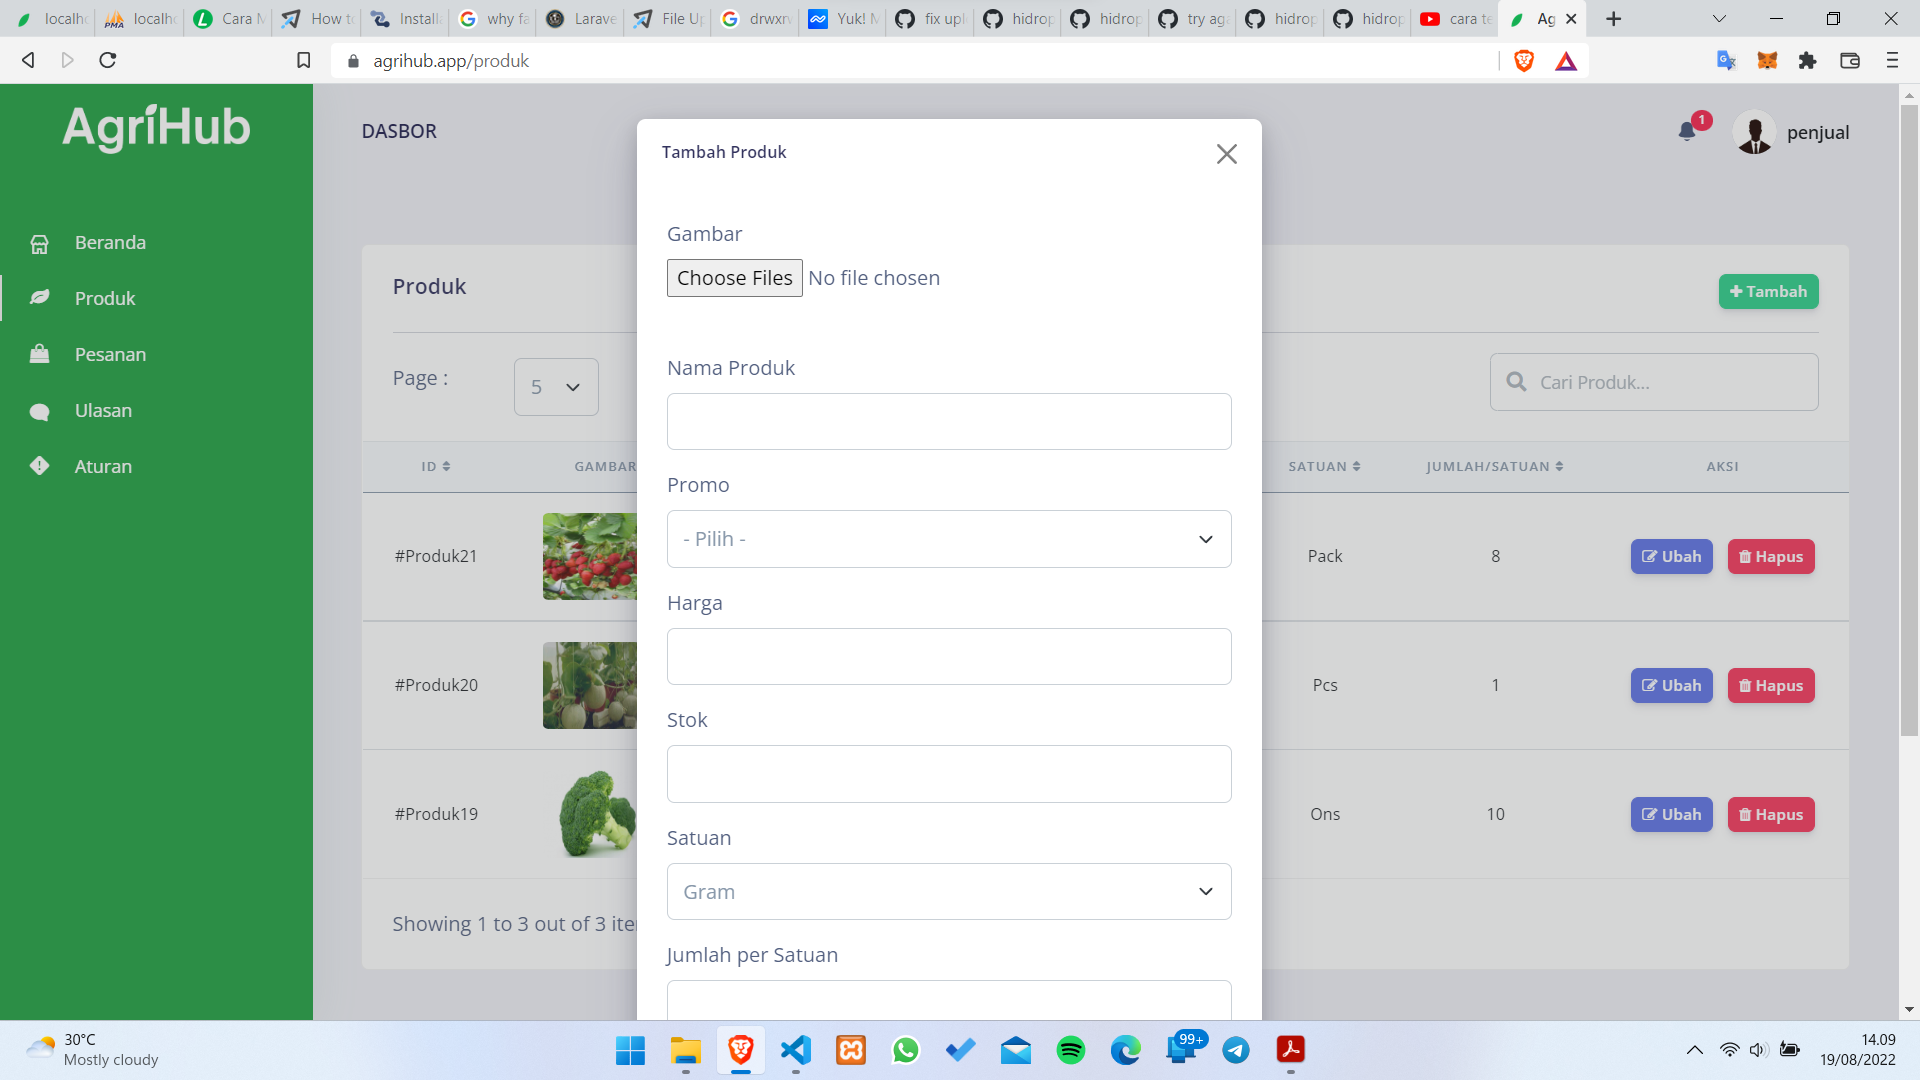
\includegraphics [width = 13cm, height= 7.5cm]{gambar/penjual/tambah_produk}}
			\caption{Tampilan Tambah Produk}
			\label{tambah_produk}
		\end{figure}

		\item Halaman Ubah Produk
		\par Penjual dapat mengubah detail produk yang ia jual melalui halaman ubah produk ini. Di sini penjual dapat menambah atau menghapus gambar produk dan dapat mengubah detail produknya seperti nama, harga, stok, satuan dan lainnya. Halaman ubah produk dapat dilihat pada gambar \ref*{ubah_produk}.
		\begin{figure}[H]
			\centering
			{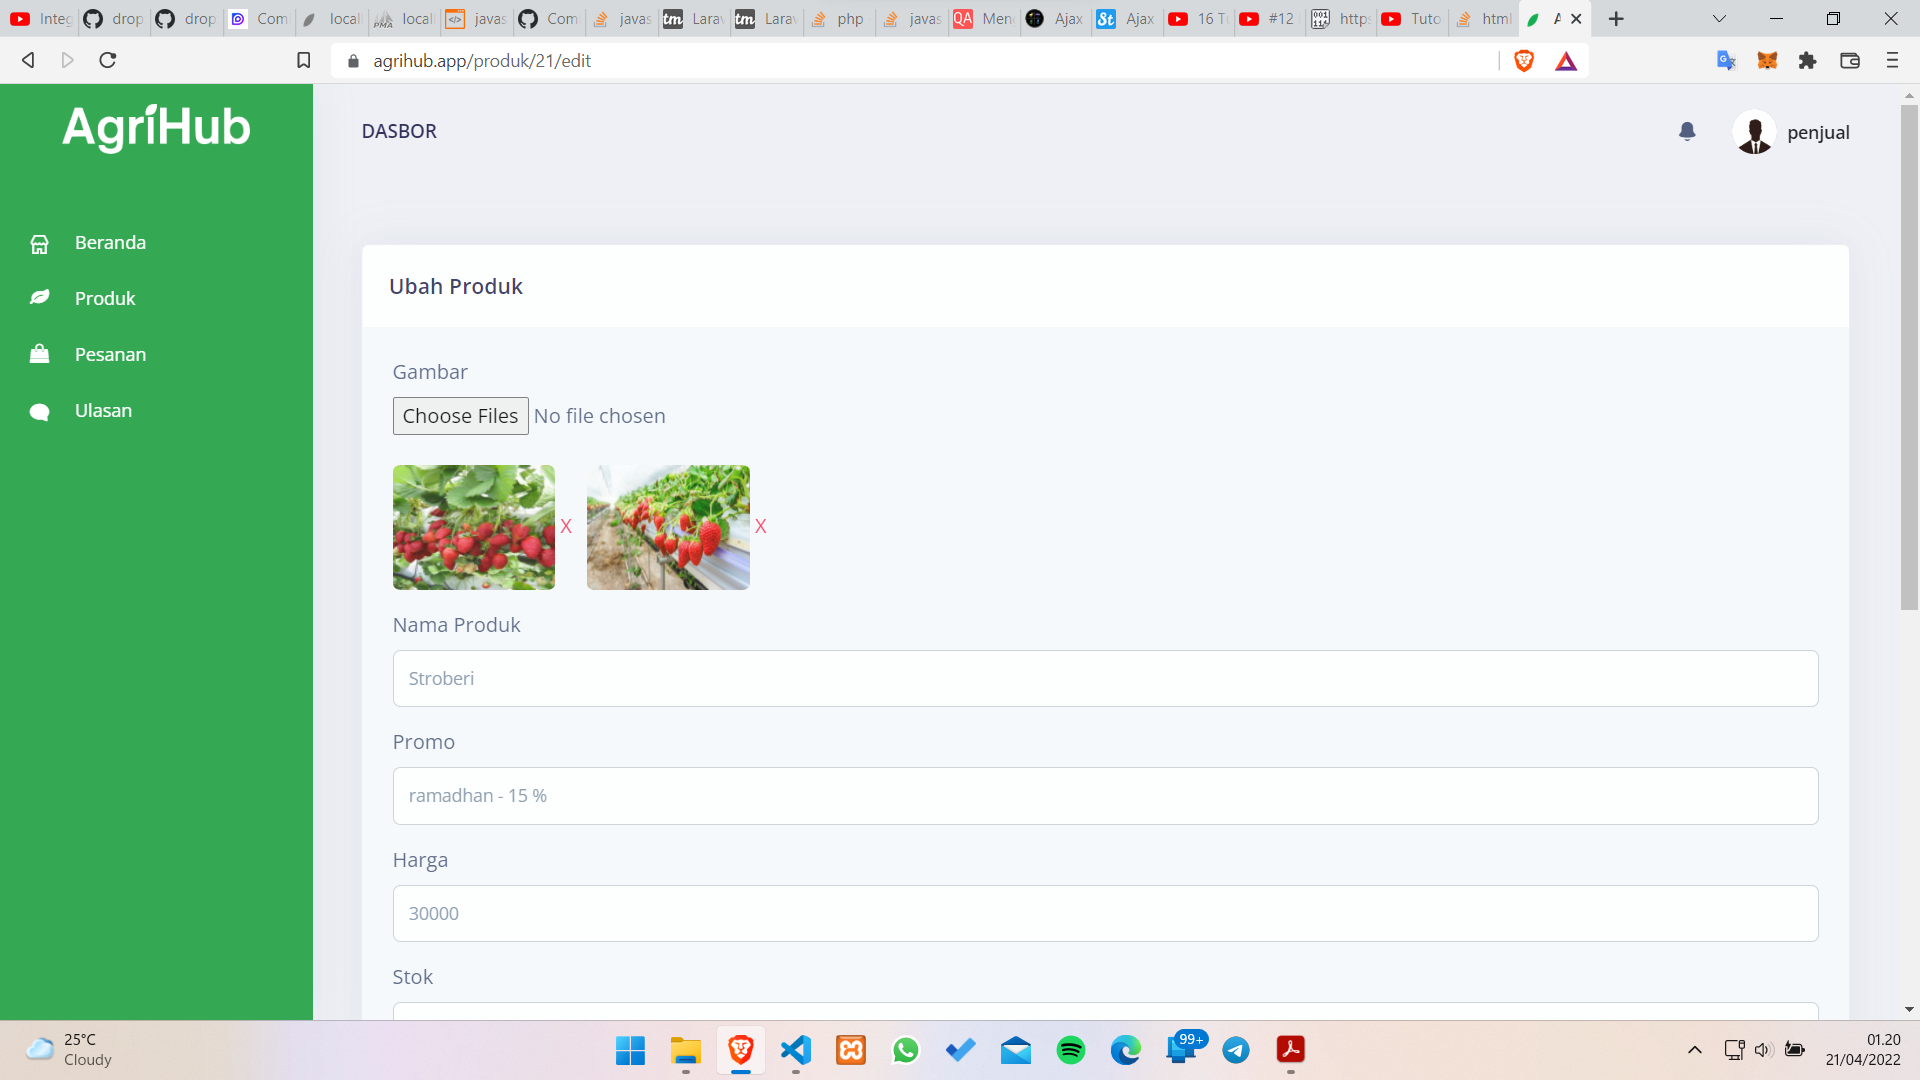
\includegraphics [width = 13cm, height= 7.5cm]{gambar/penjual/ubah_produk}}
			\caption{Halaman Ubah Produk}
			\label{ubah_produk}
		\end{figure}

		\item Halaman Pesanan
		\par Selanjutnya ada halaman pesanan, halaman ini merupakan halaman yang paling penting bagi penjual karna pada halaman ini penjual mengelola semua pesanan yang masuk dari pembeli. Penjual dapat mengetahui informasi mengenai pesanannya seperti tanggal, jam, nama pembeli, jumlah item, ongkos kirim dan total harganya beserta status pesanannya. Halaman pesanan pada sisi penjual dapat dilihat pada gambar \ref*{pesanan_penjual} dibawah ini.
		\begin{figure}[H]
			\centering
			{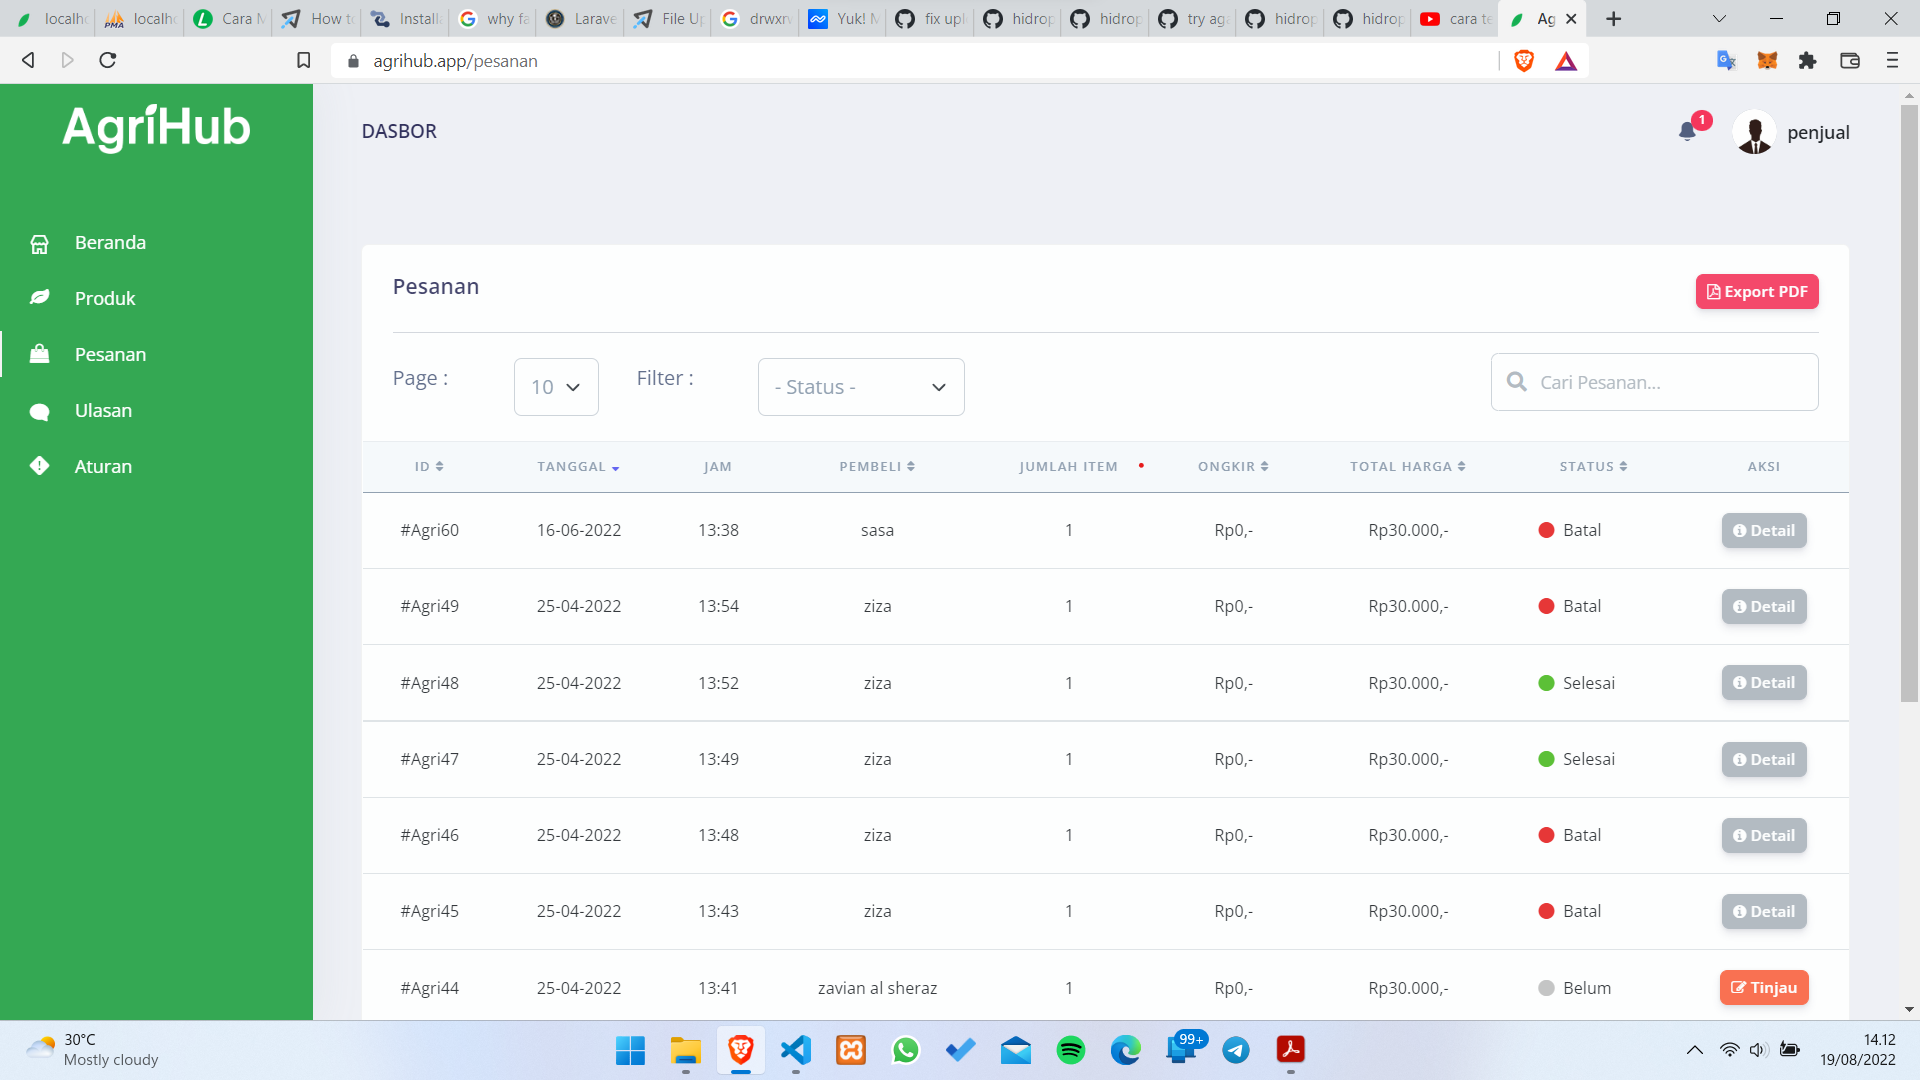
\includegraphics [width = 13cm, height= 7.5cm]{gambar/penjual/pesanan_penjual}}
			\caption{Halaman Pesanan pada sisi Penjual}
			\label{pesanan_penjual}
		\end{figure}
		\newpage
		\par Jika penjual ingin memproses pesanan dari pembeli maka dapat menekan tombol tinjau yang berwarna \textit{orange}, lalu mengisi harga ongkos kirimnya dan mengubah status pesanannya dari belum menjadi diproses. Tombol ini hanya tampil ketika status pesanannya masih belum diproses, lagi diproses dan dikirim. Namun apabila sudah selesai atau batal maka akan tampil tombol detail. Penjual dapat menghubungi pembeli di sini melalui tombol WhatApps apabila ada yang ingin ditanyakan lebih lanjut kepada pembeli. Dan penjual juga dapat menolak pesanannya dengan mengubah status pesanan menjadi batal. Tampilan tinjau pesanan dapat dilihat pada gambar \ref*{tinjau_pesanan}.
		\begin{figure}[H]
			\centering
			{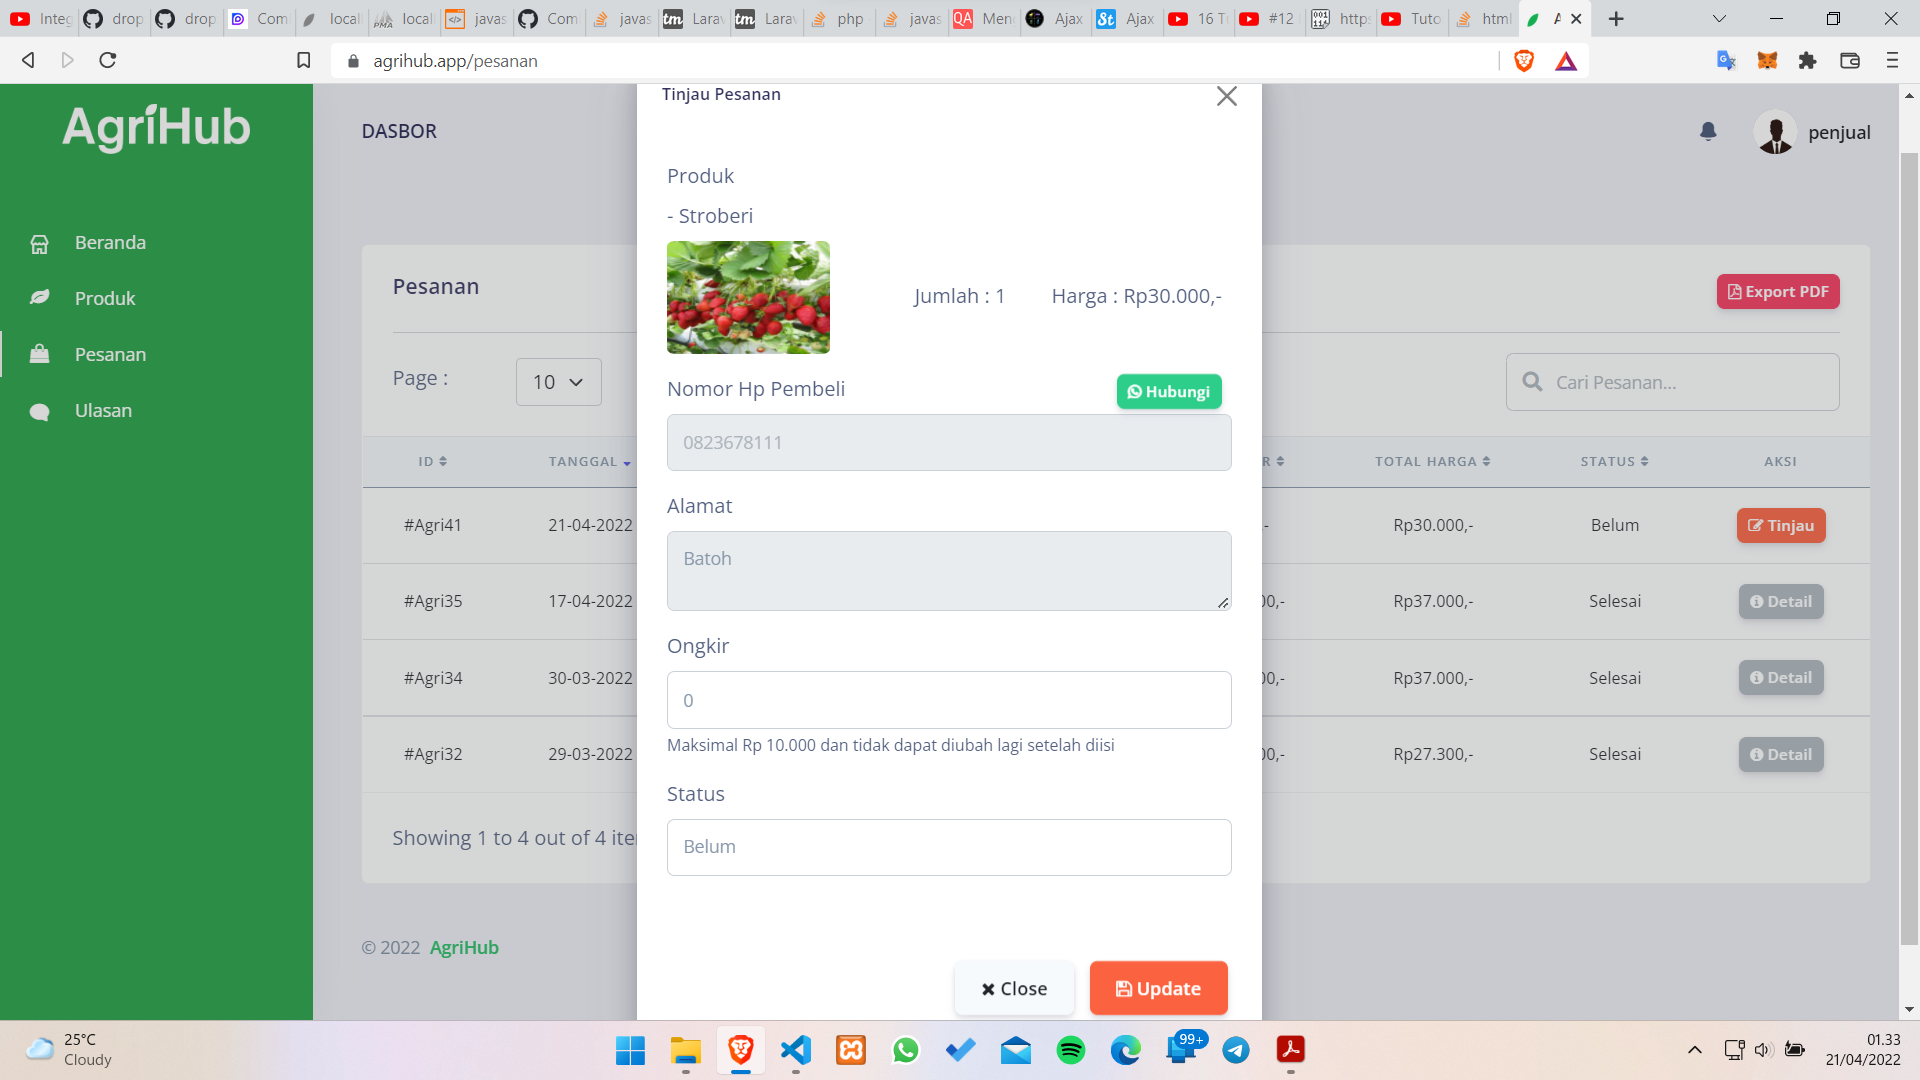
\includegraphics [width = 13cm, height= 7.5cm]{gambar/penjual/tinjau_pesanan}}
			\caption{Tampilan Tinjau Pesanan}
			\label{tinjau_pesanan}
		\end{figure}
		\par Apabila penjual ingin melihat daftar pesanannya dalam bentuk pdf dapat melakukannya dengan menekan tombol \textit{export} pdf yang berwarna merah, maka akan muncul tampilan hasilnya dalam bentuk pdf. Tampilan ekspor pdf pesanan pada sisi penjual dapat dilihat pada gambar \ref*{pdf_penjual}.
		\begin{figure}[H]
			\centering
			{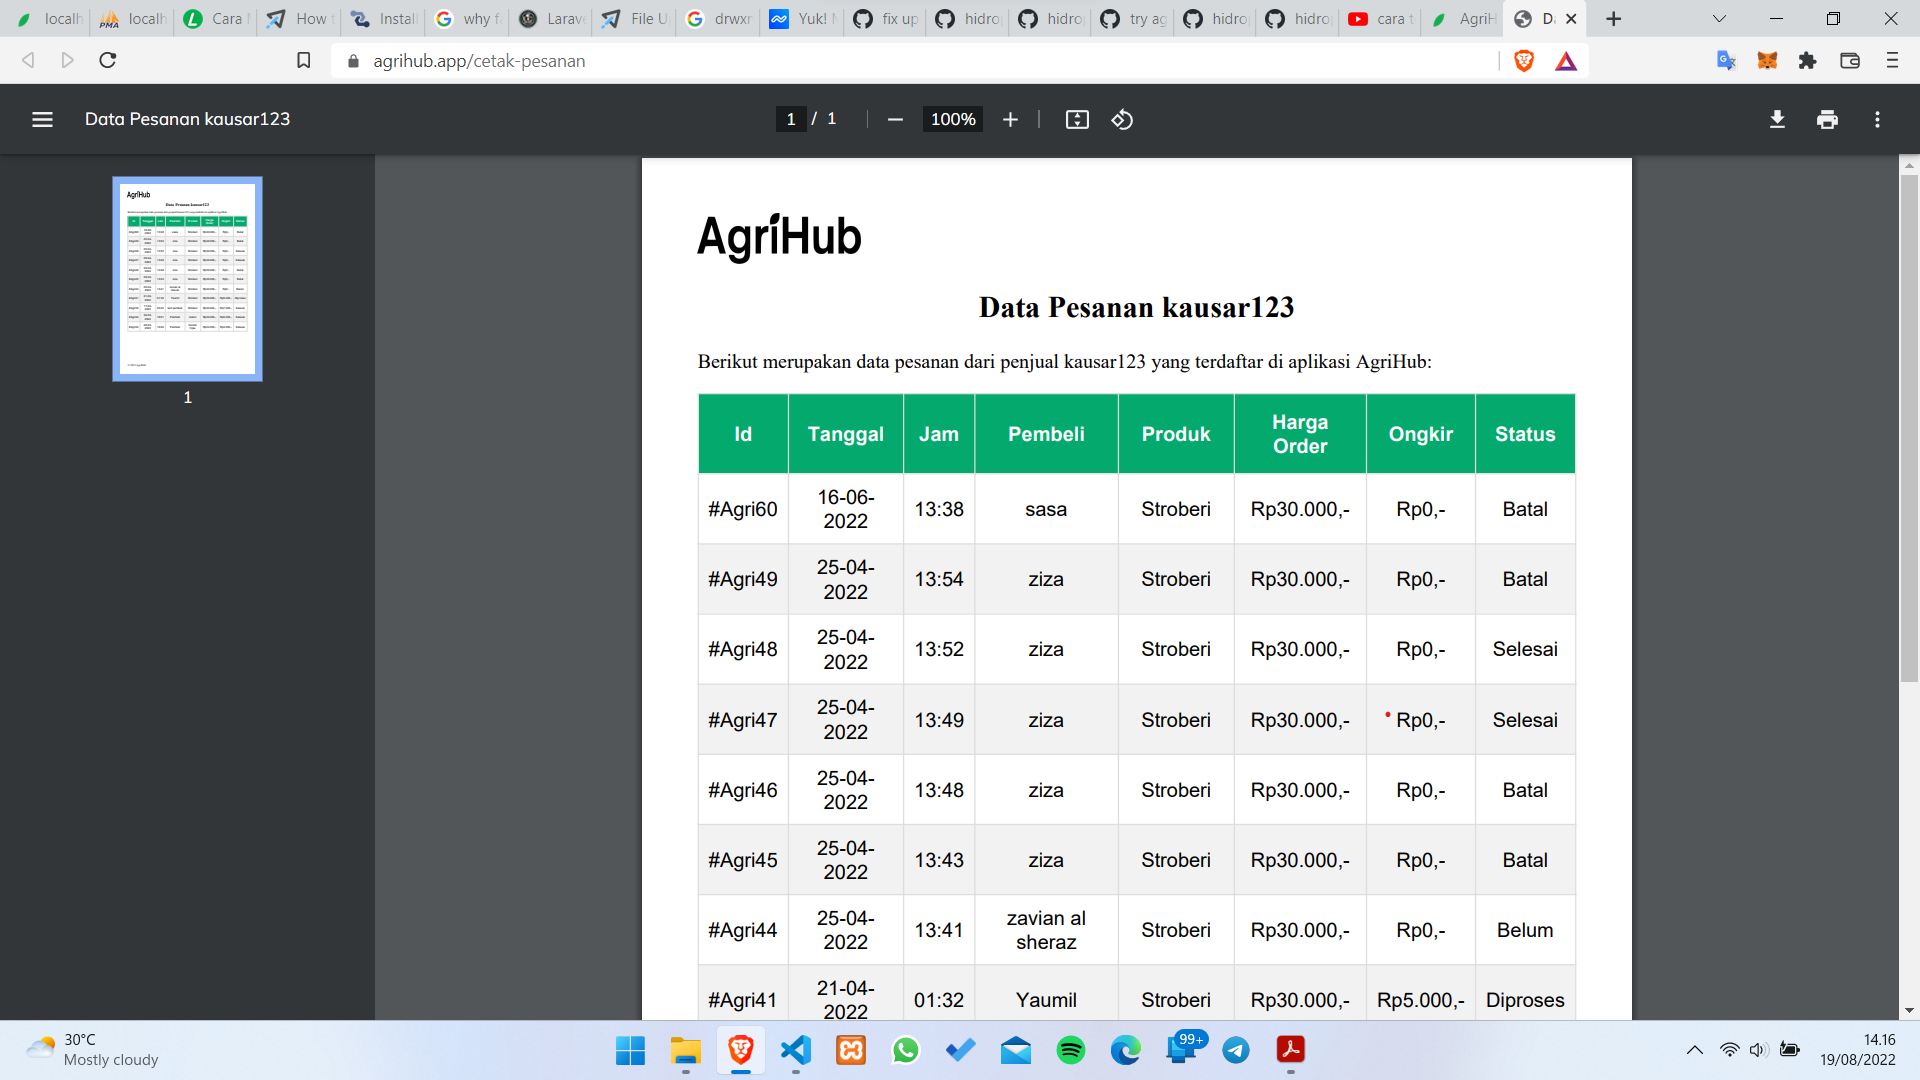
\includegraphics [width = 13cm, height= 7.5cm]{gambar/penjual/pdf_penjual}}
			\caption{Tampilan Ekspor PDF Pesanan pada sisi Penjual}
			\label{pdf_penjual}
		\end{figure}

		\item Halaman Ulasan
		\par Pada halaman ulasan ini penjual dapat melihat semua ulasan yang sudah diberikan oleh pembelinya terhadap produk yang ia jual. Dari ulasan ini dapat menjadi masukan bagi penjual untuk meningkatkan lagi kualitas produk yang ia tawarkan. Penjual juga dapat memfilter ulasannya berdasarkan ratingnya dan dapat menghapus ulasan dari pembeli jika dinilai ulasannya mengandung kata-kata yang tidak pantas. Halaman ulasan pada sisi penjual dapat dilihat pada gambar \ref*{ulasan}.
		\begin{figure}[H]
			\centering
			{\includegraphics [width = 13cm, height= 7.5cm]{gambar/penjual/ulasan}}
			\caption{Halaman Ulasan pada sisi Penjual}
			\label{ulasan}
		\end{figure}

		\newpage
		\item Halaman Ubah Profil
		\par Terakhir ada halaman profil yaitu halaman di mana penjual dapat mengubah informasi mengenai akunnya seperti foto, nama, nomor hp dan alamat serta \textit{password}. Halaman ubah profil dapat dilihat pada gambar \ref*{profil}.
		\begin{figure}[H]
			\centering
			{\includegraphics [width = 13cm, height= 7.5cm]{gambar/penjual/profil}}
			\caption{Halaman Ubah Profil}
			\label{profil}
		\end{figure}
	\end{enumerate}
\end{enumerate}

\section{\uppercase{Implementasi Sistem}}
Aplikasi penjualan tanaman hidroponik berbasis web dibangun
menggunakan \textit{framework} Laravel sebagai alat (\textit{tool}) untuk membangun aplikasi dan \textit{database} MySQL sebagai penyimpanan datanya. Pada aplikasi ini juga dibuatkan API untuk menghubungkan aplikasi Android dengan aplikasi web yang bertindak sebagai \textit{web service} untuk digunakan pada aplikasi berbasis Android. Aplikasi penjualan tanaman hidroponik ini juga sudah memiliki sertifikat Hak Kekayaan Intelektual (HKI) dengan nomor EC00202153108 yang dapat dilihat pada lampiran 1.

% \par Adapun proses implementasi sistem menggunakan metode \textit{Scrum}. Metode \textit{Scrum} terdiri dari kumpulan \textit{product backlog} yang merupakan daftar tugas yang harus dikerjakan dengan prioritasnya masing-masing. Kemudian kumpulan \textit{product backlog} tersebut diimplementasikan dalam bentuk kode pemrograman yang dibagi dalam beberapa kali iterasi atau disebut \textit{sprint}. Pada penelitian ini, terdapat 4 kali iterasi \textit{sprint}. Berikut merupakan pembagian \textit{product backlog} ke dalam beberapa iterasi :

\par Adapun proses implementasi sistem menggunakan metode Scrum. Metode Scrum terdiri dari \textit{product backlog} yang berisi daftar fitur yang akan diterapkan ke dalam aplikasi. \textit{Product backlog} dibuat berdasarkan \textit{user story} yang telah diperoleh pada hasil analisis kebutuhan pengguna. Kemudian \textit{product backlog} tersebut diimplementasikan dalam bentuk kode program yang dibagi dalam beberapa kali iterasi atau disebut \textit{sprint}. Pada penelitian ini, terdapat 4 kali iterasi. Berikut merupakan pembagian \textit{product backlog} ke dalam beberapa iterasi :

% Metode \textit{Scrum} terdiri dari kumpulan \textit{product backlog} yang merupakan daftar pekerjaan yang harus dikerjakan dengan prioritasnya masing-masing.

% Metode \textit{Scrum} terdiri dari \textit{product backlog} yang berisi daftar dari fitur yang akan diterapkan ke dalam sistem.

% \textit{Product backlog} dibuat berdasarkan \textit{user story} yang telah diperoleh pada hasil analisis kebutuhan pengguna.

\newpage
\begin{enumerate}
	\item \textit{Sprint} Pertama
	\par Pada \textit{sprint} pertama ini, merupakan tahap awal pembuatan aplikasi seperti membuat \textit{file migration} untuk \textit{database}, \textit{Models} untuk setiap tabel dan relasinya, fungsi \textit{login}, fitur \textit{upload} produk dan beberapa tampilan (\textit{view}) halaman aplikasi serta API dasar untuk digunakan pada aplikasi Android. Adapun daftar \textit{product backlog} pada \textit{sprint} yang pertama dapat dilihat pada tabel \ref*{tab:sprint pertama} berikut ini.

	% fitur yang difokuskan pada \textit{sprint} ini merupakan fitur-fitur dengan prioritas tinggi seperti membuat file migration untuk database, buat fungsi login dan beberapa view halaman serta API dasar untuk digunakan pada aplikasi Android. Adapun untuk daftar \textit{product backlog} pada \textit{sprint} yang pertama dapat dilihat pada tabel \ref*{tab:sprint pertama} berikut ini.

	\addtocounter{table}{+1}
	\begin{table}[H]
		\begin{center}
		\caption{\textit{Product Backlog sprint} pertama}
		\label{tab:sprint pertama}
		% \footnotesize
		\begin{tabular}{|l|c|}
		\hline
		\multicolumn{1}{|c|}{Item} & Prioritas\\
		\hline
		Buat \textit{file migration} untuk \textit{database} & Tinggi\\
		\hline
		Buat \textit{Models} untuk setiap tabel dan relasinya & Tinggi\\
		\hline
		Implementasi \textit{template bootstrap} Argon & Rendah\\
		\hline
		Buat \textit{role user} admin dan penjual & Tinggi\\
		\hline
		fungsi \textit{login} dua arah & Tinggi\\
		\hline
		Modifikasi halaman dasbor admin dan penjual & Sedang\\
		\hline
		\textit{view} halaman produk & Sedang\\
		\hline
		fitur \textit{upload} produk untuk penjual& Tinggi\\
		\hline
		fitur ubah dan hapus produk & Tinggi\\
		\hline
		\textit{view} halaman pesanan & Sedang\\
		\hline
		fitur proses pesanan untuk penjual & Tinggi\\
		\hline
		\textit{view} halaman pengguna untuk admin & Sedang\\
		\hline
		API \textit{login} dan \textit{register} untuk Android & Tinggi\\
		\hline
		API \textit{get} dan \textit{post} produk untuk Android & Tinggi\\
		\hline
		API \textit{get} dan \textit{post} pesanan untuk Android & Tinggi\\
		\hline
		\end{tabular}
		% \normalsize
		\end{center}
	\end{table}

	\par Kendala yang dihadapi pada \textit{sprint} pertama ini yaitu belum sinkronnya aplikasi web dan Android dikarenakan belum adanya \textit{server} resmi yang disediakan untuk aplikasi penjualan tanaman hidroponik berbasis web ini. Sehingga untuk sementara waktu, aplikasi penjualan tanaman hidroponik berbasis web ini menggunakan \textit{hosting} milik pribadi. Hal ini harus dilakukan karena agar API dari aplikasi web dapat diakses oleh aplikasi Android maka harus terlebih dahulu melakukan \textit{deployment} aplikasi berbasis web ke \textit{server} atau \textit{hosting}. Berikut ini merupakan contoh potongan kode program API untuk \textit{register user} yang sudah dibuat.
	
	% sehingga membuat aplikasi Android belum dapat mengakses datanya.

	\newpage

	\begin{lstlisting}[caption=Potongan kode program API \textit{register user}, label=lst:register]
public function register(Request $request)
{
	$validator = Validator::make($request->all(), [
		'nama_lengkap' => 'required',
		'email' => 'required|email|unique:users',
		'nomor_hp' => 'required|max:13',
		'password' => 'required',
		'username' => 'required|unique:users'
	]);

	if ($validator->fails()) {
		return response()->json(['message' => $validator->errors(), 'type' => 'failed', 'user' => '', 'token' => '']);
	}

	$data = $request->validate([
		'nama_lengkap' => 'required',
		'email' => 'required|email|unique:users',
		'nomor_hp' => 'required|max:13',
		'password' => 'required',
		'username' => 'required|unique:users'
	]);

	$data['level'] = 'pembeli';
	$data['status'] = 1;
	$data['alamat'] = '';
	$data['password'] = Hash::make($data['password']);

	$user = User::create($data);
	$token = Str::random(50);

	$users = [
		'id' => $user->id,
		'nama_lengkap' => $user->nama_lengkap,
	];
	Mail::to($user->email)->send(new \App\Mail\VerifyMail($users));
	return response()->json(['message' => $data['nama_lengkap'] . ' berhasil membuat akun', 'user' => $user, 'type' => 'success', 'token' => $token, 'verified' => $user->hasVerifiedEmail()]);
}	\end{lstlisting}

	\newpage

	\item \textit{Sprint} Kedua
	\par Pada \textit{sprint} kedua ini, dilakukan \textit{deployment} aplikasi berbasis web ini ke \textit{server} yang disediakan agar aplikasinya \textit{online} dan APInya dapat diakses oleh aplikasi Android untuk saling terhubung. Kemudian dilakukan penyempurnaan pada fitur sebelumnya seperti bisa mengunggah lebih dari 1 gambar produk dan penambahan fitur lainnya seperti fitur tambah pengguna oleh admin, promo, pencarian data dan blokir penjual. Daftar \textit{product backlog} pada \textit{sprint} kedua dapat dilihat pada tabel \ref*{tab:sprint kedua} berikut ini.
	
	% lalu dilanjutkan pembuatan fitur lainnya seperti pembuatan fitur upload produk, tambah pengguna oleh user admin, fitur promo, search dan Handling tidak bisa blokir penjual jika lagi ada pesanan.

	% dilakukan penyempurnaan dari fitur-fitur yang telah dibuat pada \textit{sprint} pertama seperti pembuatan fitur upload produk, tambah pengguna oleh user admin, fitur promo, search dan Handling tidak bisa blokir penjual jika lagi ada pesanan. Tingkat prioritas pada tahap \textit{sprint} kedua didominasi oleh tingkatan prioritas sedang. Daftar \textit{product backlog} pada \textit{sprint} kedua dapat dilihat pada tabel \ref*{tab:sprint kedua} berikut ini.

	\begin{table}[H]
		\begin{center}
		\caption{\textit{Product Backlog sprint} kedua}
		\label{tab:sprint kedua}
		% \footnotesize
		\begin{tabular}{|l|c|}
		\hline
		\multicolumn{1}{|c|}{Item} & Prioritas\\
		\hline
		\textit{Deploy} aplikasi ke \textit{server} & Tinggi\\
		\hline
		fitur \textit{upload multiple image} produk & Tinggi\\
		\hline
		fitur tambah pengguna & Tinggi\\
		\hline
		\textit{view} halaman promo untuk admin & Sedang\\
		\hline
		fitur buat promo di aplikasi & Sedang\\
		\hline
		fitur ubah dan hapus promo & Sedang\\
		\hline
		fitur ubah profil akun dan foto & Tinggi\\
		\hline
		fitur pencarian data & Tinggi\\
		\hline
		buat \textit{pagination} & Sedang\\
		\hline
		fitur blokir akun penjual & Tinggi\\
		\hline
		\textit{view} halaman laporan & Sedang\\
		\hline
		API \textit{get} dan \textit{post} laporan & Sedang\\
		\hline
		\textit{view} halaman ulasan & Sedang\\
		\hline
		API \textit{get} dan \textit{post} ulasan & Sedang\\
		\hline
		\textit{view} halaman informasi & Rendah\\
		\hline
		\textit{view} halaman \textit{privacy policy} & Rendah\\
		\hline
		\end{tabular}
		% \normalsize
		\end{center}
	\end{table}

	\item \textit{Sprint} Ketiga
	\par Pada \textit{sprint} ketiga ini, dilakukan pemasangan nama domain pada aplikasi web ini dikarenakan sebelumnya masih berbentuk alamat IP. Kemudian dilakukan penambahan fitur keamanan seperti verifikasi email untuk penjual, perbaikan \textit{bug} logika di menu pesanan dikarenakan sebelumnya pembeli tidak dapat membeli lebih dari 1 jenis produk sekaligus dalam 1 kali pesanan, \textit{update database} dan \textit{handling} produk supaya tidak bisa dihapus oleh penjual atau admin jika lagi dipesan oleh pembeli. Daftar \textit{product backlog} pada \textit{sprint} ketiga dapat dilihat pada tabel \ref*{tab:sprint ketiga} berikut ini.
	
	% dan penambahan fitur keamanan seperti verifikasi email oleh penjual

	% dilakukan penambahan beberapa fitur seperti verifikasi email oleh penjual, perbaikan bug logika di menu pesanan dikarenakan sebelumnya pembeli tidak dapat membeli lebih dari 1 jenis produk sekaligus dalam 1 pesanan, 
	
	% update database dan handling produk supaya tidak bisa dihapus oleh penjual atau admin jika lagi dipesan oleh pembeli. Tingkat prioritas pada tahap \textit{sprint} ketiga didominasi oleh tingkatan prioritas sedang. Daftar \textit{product backlog} pada \textit{sprint} ketiga dapat dilihat pada tabel \ref*{tab:sprint ketiga} berikut ini.

	\begin{table}[H]
		\begin{center}
		\caption{\textit{Product Backlog sprint} ketiga}
		\label{tab:sprint ketiga}
		% \footnotesize
		\begin{tabular}{|l|c|}
		\hline
		\multicolumn{1}{|c|}{Item} & Prioritas\\
		\hline
		Pasang nama \textit{domain website} & Sedang\\
		\hline
		\textit{Handling} tidak bisa blokir penjual yang lagi ada pesanan diproses & Tinggi\\
		\hline
		fitur verifikasi email penjual & Tinggi\\
		\hline
		fitur lupa \textit{password} & Tinggi\\
		\hline
		Perbaiki \textit{bug} logika di menu pesanan & Tinggi\\
		\hline
		\textit{Update database} tambahkan tabel \textit{orderMappings} & Tinggi\\
		\hline
		\textit{Update view} pesanan & Sedang\\
		\hline
		\textit{Handling} tidak bisa hapus produk yang lagi dipesan pembeli & Tinggi\\
		\hline
		Tambah logo dan \textit{ganti background} halaman utama & Rendah\\
		\hline
		\end{tabular}
		% \normalsize
		\end{center}
	\end{table}

	\item \textit{Sprint} Keempat
	\par Pada \textit{sprint} keempat ini, dilakukan penambahan beberapa fitur pelengkap pada aplikasi supaya lebih fungsional lagi seperti fitur memfilter data, \textit{sorting} data, grafik, notifikasi dan ekspor pdf. Daftar \textit{product backlog} pada \textit{sprint} keempat dapat dilihat pada tabel \ref*{tab:sprint keempat} berikut ini.

	\begin{table}[H]
		\begin{center}
		\caption{\textit{Product Backlog sprint} keempat}
		\label{tab:sprint keempat}
		% \footnotesize
		\begin{tabular}{|l|c|}
		\hline
		\multicolumn{1}{|c|}{Item} & Prioritas\\
		\hline
		fitur filter data dan \textit{sort} data dengan \textit{datatable} & Tinggi\\
		\hline
		fitur grafik pada dasbor admin dan penjual & Tinggi\\
		\hline
		fitur notifikasi pesanan, stok produk dan laporan & Sedang\\
		\hline
		fitur ekspor pesanan dalam bentuk pdf & Sedang\\
		\hline
		tambah kolom jam pemesanan di \textit{view} pesanan & Rendah\\
		\hline
		\end{tabular}
		% \normalsize
		\end{center}
	\end{table}

	\par Berikut ini akan ditampilkan struktur folder dari Laravel. Terdiri dari beberapa folder konfigurasi aplikasi, folder \textit{app} merupakan folder utama yang berisi folder dan \textit{file} yang berhubungan dengan aplikasi seperti \textit{Controller} dan \textit{Models}, folder \textit{public} berisi \textit{assets} seperti \textit{file} css, logo, dan \textit{file} \textit{javascript} serta gambar yang diunggah oleh pengguna. Folder \textit{storage} untuk menyimpan data gambar, folder \textit{database} untuk menyimpan berkas basis data seperti \textit{migration}, folder \textit{routes} untuk menyimpan berkas yang menjadi pengarah navigasi halaman, folder \textit{resources} untuk menyimpan berkas yang akan menjadi tampilan pada aplikasi. Gambaran struktur folder pembuatan aplikasi dapat dilihat pada gambar \ref*{struktur folder}.

	\begin{figure}[H]
		\centering
		{\includegraphics [width = 5cm, height= 13cm]{gambar/struktur folder}}
		\caption{Struktur Folder}
		\label{struktur folder}
	\end{figure}
\end{enumerate}

\section{\uppercase{Pengujian Sistem}}
Pengujian sistem atau aplikasi sangat perlu dilakukan mengingat setiap pengembangan aplikasi tidak terlepas dari kesalahan (\textit{bug}), perbaikan dan pengembangan lanjutan. Maka diperlukan pengujian sistem untuk mendapati kesalahan tersebut agar dapat diperbaiki dan untuk melihat apakah sistem tersebut sudah berjalan dengan baik dan sesuai yang diharapkan. Pada penelitian ini akan dilakukan 2 pengujian yaitu pengujian fungsionalitas dengan metode \textit{black box} dan pengujian \textit{usability} dengan metode UMUX.

\subsection{Pengujian Fungsionalitas Menggunakan Black Box}
Pengujian fungsionalitas dilakukan untuk mengetahui apakah aplikasi penjualan tanaman hidroponik berbasis web sudah berfungsi dengan baik atau belum. Metode yang digunakan pada pengujian fungsionalitas ini yaitu metode \textit{black box}. Metode ini hanya akan berfokus pada fungsi aplikasi tanpa memperhatikan struktur \textit{code} di dalam aplikasi. Pada penelitian ini pengujian fungsionalitas dilakukan secara manual dengan penguji yang akan bertindak sebagai pengguna aplikasi. Hasil pengujian \textit{black box} dapat dilihat pada tabel \ref*{tab:black box} di bawah ini.

% \begin{table}[H]
% 	\begin{center}
% 	\caption{Tabel Black Box}
% 	\label{tab:black box}
% 	% \footnotesize
% 	\begin{tabular}{| m{0.6cm} | m{3.3cm} | m{3.3cm} | m{3.3cm} | m{1.6cm} |}
% 	\hline
% 	{\footnotesize No.} & \multicolumn{1}{|c|}{{\footnotesize Nama Pengujian}}  & \multicolumn{1}{|c|}{{\footnotesize Skenario}} & \multicolumn{1}{|c|}{{\footnotesize Tampilan}} & {\footnotesize Kesimpulan}\\
% 	\hline
% 	{\footnotesize 1} & {\footnotesize Melakukan masuk akun} & {\footnotesize Mengisi semua data yang
% 	sesuai dengan database} & {\footnotesize Diarahkan ke halaman dasbor} & \multicolumn{1}{|c|}{{\footnotesize Sesuai}}\\
% 	\hline
% 	{\footnotesize 2} & {\footnotesize Melakukan masuk akun} & {\footnotesize Mengisi data yang
% 	tidak ada di database} & {\footnotesize Peringatan data
% 	tidak valid} & \multicolumn{1}{|c|}{{\footnotesize Sesuai}}\\
% 	\hline
% 	{\footnotesize 3} & {\footnotesize Melakukan masuk akun} & {\footnotesize Tidak mengisi salah satu
% 	atau semua data} & {\footnotesize Peringatan data
% 	belum diisi} & \multicolumn{1}{|c|}{{\footnotesize Sesuai}}\\
% 	\hline
% 	{\footnotesize 4} & {\footnotesize Mengubah profil akun} & {\footnotesize Mengisi data dengan input
% 	yang valid} & {\footnotesize Diarahkan kembali ke
% 	halaman profil} & \multicolumn{1}{|c|}{{\footnotesize Sesuai}}\\
% 	\hline
% 	{\footnotesize 5} & {\footnotesize Mengubah profil akun} & {\footnotesize Mengisi data dengan input
% 	yang tidak valid} & {\footnotesize Peringatan data
% 	tidak valid} & \multicolumn{1}{|c|}{{\footnotesize Sesuai}}\\
% 	\hline
% 	{\footnotesize 6} & {\footnotesize Mencari produk yang
% 	diinginkan} & {\footnotesize Memasukkan kata kunci dikolom pencarian sesuai yang tersedia di database} & {\footnotesize Hasil pencarian
% 	ditampilkan} & \multicolumn{1}{|c|}{{\footnotesize Sesuai}}\\
% 	\hline
% 	{\footnotesize 7} & {\footnotesize Mencari produk yang
% 	diinginkan} & {\footnotesize Memasukkan kata kunci dikolom pencarian yang tidak tersedia di database} & {\footnotesize Tampilan pencarian
% 	tidak ditemukan} & \multicolumn{1}{|c|}{{\footnotesize Sesuai}}\\
% 	\hline
% 	{\footnotesize 8} & {\footnotesize Melakukan pendaftaran akun penjual} & {\footnotesize Mengisi semua data yang valid} & {\footnotesize Muncul pop up berhasil} & \multicolumn{1}{|c|}{{\footnotesize Sesuai}}\\
% 	\hline
% 	{\footnotesize 9} & {\footnotesize Melakukan pendaftaran akun penjual} & {\footnotesize Mengisi salah satu data dengan input yang tidak sesuai} & {\footnotesize Peringatan data tidak valid} & \multicolumn{1}{|c|}{{\footnotesize Sesuai}}\\
% 	\hline
% 	{\footnotesize 10} & {\footnotesize Melakukan pendaftaran akun penjual} & {\footnotesize Tidak mengisi salah satu atau semua data} & {\footnotesize Peringatan data belum diisi} & \multicolumn{1}{|c|}{{\footnotesize Sesuai}}\\
% 	\hline
% 	{\footnotesize 11} & {\footnotesize Menambahkan produk yang ingin dijual} & {\footnotesize Mengisi semua data dengan valid} & {\footnotesize Produk ditambahkan
% 	pada halaman produk} & \multicolumn{1}{|c|}{{\footnotesize Sesuai}}\\
% 	\hline
% 	\end{tabular}
% 	% \normalsize
% 	\end{center}
% \end{table}

% \newpage

% \addtocounter{table}{-1}
% \begin{table}[H]
% 	\begin{center}
% 	% \caption[]{Tabel Black Box}
% 	% \label{tab:jadwal}
% 	% \footnotesize
% 	\begin{tabular}{| m{0.6cm} | m{3.3cm} | m{3.3cm} | m{3.3cm} | m{1.6cm} |}
% 	\hline
% 	{\footnotesize No.} & \multicolumn{1}{|c|}{{\footnotesize Nama Pengujian}}  & \multicolumn{1}{|c|}{{\footnotesize Skenario}} & \multicolumn{1}{|c|}{{\footnotesize Tampilan}} & {\footnotesize Kesimpulan}\\
% 	\hline
% 	{\footnotesize 12} & {\footnotesize Menambahkan produk yang ingin dijual} & {\footnotesize Mengisi salah satu data dengan input yang tidak sesuai} & {\footnotesize Peringatan data tidak valid dan kembali ke halaman produk} & \multicolumn{1}{|c|}{{\footnotesize Sesuai}}\\
% 	\hline
% 	{\footnotesize 13} & {\footnotesize Menambahkan produk yang ingin dijual} & {\footnotesize Tidak mengisi salah satu atau semua data} & {\footnotesize Peringatan data tidak valid dan kembali ke halaman produk} & \multicolumn{1}{|c|}{{\footnotesize Sesuai}}\\
% 	\hline
% 	{\footnotesize 13} & {\footnotesize Mengubah produk} & {\footnotesize Mengisi data dengan input yang valid} & {\footnotesize Diarahkan kembali ke halaman produk} & \multicolumn{1}{|c|}{{\footnotesize Sesuai}}\\
% 	\hline
% 	{\footnotesize 15} & {\footnotesize Mengubah produk} & {\footnotesize Mengisi data dengan input yang tidak valid} & {\footnotesize Peringatan data tidak valid dan kembali ke halaman produk} & \multicolumn{1}{|c|}{{\footnotesize Sesuai}}\\
% 	\hline
% 	{\footnotesize 16} & {\footnotesize Menghapus produk} & {\footnotesize klik tombol hapus pada produk yang tidak sedang dibeli} & {\footnotesize Terhapus dari daftar produk} & \multicolumn{1}{|c|}{{\footnotesize Sesuai}}\\
% 	\hline
% 	{\footnotesize 17} & {\footnotesize Menghapus produk} & {\footnotesize klik tombol hapus pada produk yang sedang dalam proses beli} & {\footnotesize Muncul alert produk sedang dalam pembelian} & \multicolumn{1}{|c|}{{\footnotesize Sesuai}}\\
% 	\hline
% 	\end{tabular}
% 	% \normalsize
% 	\end{center}
% \end{table}

\begin{longtable}{| m{0.5cm} | m{3.2cm} | m{3.4cm} | m{3.3cm} | m{1.6cm} |}
	\caption{Tabel Black Box}
	\label{tab:black box}\\
	\hline
	{\footnotesize No.} & \multicolumn{1}{|c|}{{\footnotesize Nama Pengujian}}  & \multicolumn{1}{|c|}{{\footnotesize Skenario}} & \multicolumn{1}{|c|}{{\footnotesize Tampilan}} & {\footnotesize Kesimpulan}\\
	\hline
	\multicolumn{1}{|c|}{{\footnotesize 1}} & {\footnotesize Melakukan masuk akun} & {\footnotesize Mengisi data yang sesuai dengan \textit{database}} & {\footnotesize Diarahkan ke halaman dasbor} & \multicolumn{1}{|c|}{{\footnotesize Sesuai}}\\
	\hline
	\multicolumn{1}{|c|}{{\footnotesize 2}} & {\footnotesize Melakukan masuk akun} & {\footnotesize Mengisi data yang tidak ada di \textit{database}} & {\footnotesize Peringatan data tidak valid} & \multicolumn{1}{|c|}{{\footnotesize Sesuai}}\\
	\hline
	\multicolumn{1}{|c|}{{\footnotesize 3}} & {\footnotesize Melakukan masuk akun} & {\footnotesize Tidak mengisi salah satu atau semua data} & {\footnotesize Peringatan data belum diisi} & \multicolumn{1}{|c|}{{\footnotesize Sesuai}}\\
	\hline
	\multicolumn{1}{|c|}{{\footnotesize 4}} & {\footnotesize Melihat daftar produk} & {\footnotesize Menklik pada menu produk} & {\footnotesize Diarahkan ke halaman produk} & \multicolumn{1}{|c|}{{\footnotesize Sesuai}}\\
	\hline
	\multicolumn{1}{|c|}{{\footnotesize 5}} & {\footnotesize Menambahkan produk yang ingin dijual} & {\footnotesize Mengisi semua data dengan valid} & {\footnotesize Produk ditambahkan pada halaman produk} & \multicolumn{1}{|c|}{{\footnotesize Sesuai}}\\
	\hline
	\multicolumn{1}{|c|}{{\footnotesize 6}} & {\footnotesize Menambahkan produk yang ingin dijual} & {\footnotesize Mengisi salah satu data dengan input yang tidak sesuai} & {\footnotesize Peringatan data tidak valid dan kembali ke halaman produk} & \multicolumn{1}{|c|}{{\footnotesize Sesuai}}\\
	\hline
	\multicolumn{1}{|c|}{{\footnotesize 7}} & {\footnotesize Menambahkan produk yang ingin dijual} & {\footnotesize Tidak mengisi salah satu atau semua data} & {\footnotesize Peringatan data tidak valid dan kembali ke halaman produk} & \multicolumn{1}{|c|}{{\footnotesize Sesuai}}\\
	\hline
	\multicolumn{1}{|c|}{{\footnotesize 8}} & {\footnotesize Mengubah produk} & {\footnotesize Mengisi data dengan input yang valid} & {\footnotesize Diarahkan kembali ke halaman produk} & \multicolumn{1}{|c|}{{\footnotesize Sesuai}}\\
	\hline
	\multicolumn{1}{|c|}{{\footnotesize 9}} & {\footnotesize Mengubah produk} & {\footnotesize Mengisi data dengan input yang tidak valid} & {\footnotesize Peringatan data tidak valid dan kembali ke halaman produk} & \multicolumn{1}{|c|}{{\footnotesize Sesuai}}\\
	\hline
	\multicolumn{1}{|c|}{{\footnotesize 10}} & {\footnotesize Menghapus produk} & {\footnotesize klik tombol hapus pada produk yang tidak sedang dibeli} & {\footnotesize Terhapus dari daftar produk} & \multicolumn{1}{|c|}{{\footnotesize Sesuai}}\\
	\hline
	\multicolumn{1}{|c|}{{\footnotesize 11}} & {\footnotesize Menghapus produk} & {\footnotesize klik tombol hapus pada produk yang sedang dalam proses beli} & {\footnotesize Muncul \textit{alert} produk sedang ada pesanan} & \multicolumn{1}{|c|}{{\footnotesize Sesuai}}\\
	\hline
	\multicolumn{1}{|c|}{{\footnotesize 12}} & {\footnotesize Melihat daftar pesanan} & {\footnotesize Menklik pada menu pesanan} & {\footnotesize Diarahkan ke halaman pesanan} & \multicolumn{1}{|c|}{{\footnotesize Sesuai}}\\
	\hline
	\multicolumn{1}{|c|}{{\footnotesize 13}} & {\footnotesize Memproses pesanan} & {\footnotesize klik tombol tinjau, isi ongkos kirim dan ubah status pesanan} & {\footnotesize Pesanan berubah statusnya menjadi diproses} & \multicolumn{1}{|c|}{{\footnotesize Sesuai}}\\
	\hline
	\multicolumn{1}{|c|}{{\footnotesize 14}} & {\footnotesize Memproses pesanan} & {\footnotesize klik tombol tinjau, tidak mengisi ongkos kirim dan ubah status pesanan} & {\footnotesize Muncul \textit{alert} ongkos kirim belum diisi} & \multicolumn{1}{|c|}{{\footnotesize Sesuai}}\\
	\hline
	\multicolumn{1}{|c|}{{\footnotesize 15}} & {\footnotesize Melihat daftar promo} & {\footnotesize Menklik pada menu promo} & {\footnotesize Diarahkan ke halaman promo} & \multicolumn{1}{|c|}{{\footnotesize Sesuai}}\\
	\hline
	\multicolumn{1}{|c|}{{\footnotesize 16}} & {\footnotesize Menambahkan promo ke aplikasi} & {\footnotesize Mengisi semua data dengan valid} & {\footnotesize Promo berhasil ditambahkan} & \multicolumn{1}{|c|}{{\footnotesize Sesuai}}\\
	\hline
	\multicolumn{1}{|c|}{{\footnotesize 17}} & {\footnotesize Menambahkan promo ke aplikasi} & {\footnotesize Mengisi salah satu data dengan input yang tidak sesuai} & {\footnotesize Peringatan data tidak valid dan kembali ke halaman promo} & \multicolumn{1}{|c|}{{\footnotesize Sesuai}}\\
	\hline
	\multicolumn{1}{|c|}{{\footnotesize 18}} & {\footnotesize Menambahkan promo ke aplikasi} & {\footnotesize Tidak mengisi salah satu atau semua data} & {\footnotesize Peringatan data tidak valid dan kembali ke halaman promo} & \multicolumn{1}{|c|}{{\footnotesize Sesuai}}\\
	\hline
	\multicolumn{1}{|c|}{{\footnotesize 19}} & {\footnotesize Mengubah promo} & {\footnotesize Mengisi data dengan input yang valid} & {\footnotesize Diarahkan kembali ke halaman promo} & \multicolumn{1}{|c|}{{\footnotesize Sesuai}}\\
	\hline
	\multicolumn{1}{|c|}{{\footnotesize 20}} & {\footnotesize Mengubah promo} & {\footnotesize Mengisi data dengan input yang tidak valid} & {\footnotesize Peringatan data tidak valid dan kembali ke halaman promo} & \multicolumn{1}{|c|}{{\footnotesize Sesuai}}\\
	\hline
	\multicolumn{1}{|c|}{{\footnotesize 21}} & {\footnotesize Menghapus promo} & {\footnotesize klik tombol hapus pada promo} & {\footnotesize Terhapus dari daftar promo} & \multicolumn{1}{|c|}{{\footnotesize Sesuai}}\\
	\hline
	\multicolumn{1}{|c|}{{\footnotesize 22}} & {\footnotesize Melihat daftar pengguna} & {\footnotesize Menklik pada menu pengguna} & {\footnotesize Diarahkan ke halaman pengguna} & \multicolumn{1}{|c|}{{\footnotesize Sesuai}}\\
	\hline
	\multicolumn{1}{|c|}{{\footnotesize 23}} & {\footnotesize Melakukan pendaftaran akun penjual} & {\footnotesize Mengisi semua data yang valid} & {\footnotesize Diarahkan kembali ke halaman pengguna} & \multicolumn{1}{|c|}{{\footnotesize Sesuai}}\\
	\hline
	\multicolumn{1}{|c|}{{\footnotesize 24}} & {\footnotesize Melakukan pendaftaran akun penjual} & {\footnotesize Mengisi salah satu data dengan input yang tidak sesuai} & {\footnotesize Peringatan data tidak valid} & \multicolumn{1}{|c|}{{\footnotesize Sesuai}}\\
	\hline
	\multicolumn{1}{|c|}{{\footnotesize 25}} & {\footnotesize Melakukan pendaftaran akun penjual} & {\footnotesize Tidak mengisi salah satu atau semua data} & {\footnotesize Peringatan data belum diisi} & \multicolumn{1}{|c|}{{\footnotesize Sesuai}}\\
	\hline
	\multicolumn{1}{|c|}{{\footnotesize 26}} & {\footnotesize Memblokir akun penjual} & {\footnotesize klik tombol blokir pada data penjual} & {\footnotesize Status akun penjual berubah} & \multicolumn{1}{|c|}{{\footnotesize Sesuai}}\\
	\hline
	\multicolumn{1}{|c|}{{\footnotesize 27}} & {\footnotesize Melihat daftar keluhan} & {\footnotesize Menklik pada menu keluhan} & {\footnotesize Diarahkan ke halaman keluhan} & \multicolumn{1}{|c|}{{\footnotesize Sesuai}}\\
	\hline
	\multicolumn{1}{|c|}{{\footnotesize 28}} & {\footnotesize Melihat daftar ulasan} & {\footnotesize Menklik pada menu ulasan} & {\footnotesize Diarahkan ke halaman ulasan} & \multicolumn{1}{|c|}{{\footnotesize Sesuai}}\\
	\hline
	\multicolumn{1}{|c|}{{\footnotesize 29}} & {\footnotesize Melakukan pencarian data} & {\footnotesize Memasukkan kata kunci dikolom pencarian sesuai yang tersedia di \textit{database}} & {\footnotesize Hasil pencarian ditampilkan} & \multicolumn{1}{|c|}{{\footnotesize Sesuai}}\\
	\hline
	\multicolumn{1}{|c|}{{\footnotesize 30}} & {\footnotesize Melakukan pencarian data} & {\footnotesize Memasukkan kata kunci dikolom pencarian yang tidak tersedia di \textit{database}} & {\footnotesize Tampilan pencarian tidak ditemukan} & \multicolumn{1}{|c|}{{\footnotesize Sesuai}}\\
	\hline
	\multicolumn{1}{|c|}{{\footnotesize 31}} & {\footnotesize Melakukan \textit{sorting} data} & {\footnotesize Menklik pada nama kolom di tabel} & {\footnotesize Data diurutkan berdasarkan kolom yang dipilih} & \multicolumn{1}{|c|}{{\footnotesize Sesuai}}\\
	\hline
	\multicolumn{1}{|c|}{{\footnotesize 32}} & {\footnotesize Mengubah profil akun} & {\footnotesize Mengisi data dengan input yang valid} & {\footnotesize Diarahkan kembali ke halaman profil} & \multicolumn{1}{|c|}{{\footnotesize Sesuai}}\\
	\hline
	\multicolumn{1}{|c|}{{\footnotesize 33}} & {\footnotesize Mengubah profil akun} & {\footnotesize Mengisi data dengan input yang tidak valid} & {\footnotesize Peringatan data tidak valid} & \multicolumn{1}{|c|}{{\footnotesize Sesuai}}\\
	\hline
\end{longtable}

% \begin{longtable}{| m{0.6cm} | m{3.3cm} | m{3.3cm} | m{3.3cm} | m{1.6cm} |}
% 	\caption{Tabel Black Box}
% 	\label{tab:black box}\\
% 	\footnotesize
% 	\hline
% 	No. & \multicolumn{1}{|c|}{Nama Pengujian}  & \multicolumn{1}{|c|}{Skenario} & \multicolumn{1}{|c|}{Tampilan} & Kesimpulan\\
% 	\hline
% 	1 & Melakukan masuk akun & Mengisi semua data yang
% 	sesuai dengan database & Diarahkan ke halaman dasbor & \multicolumn{1}{|c|}{Sesuai}\\
% 	\hline
% 	2 & Melakukan masuk akun & Mengisi data yang
% 	tidak ada di database & Peringatan data
% 	tidak valid & \multicolumn{1}{|c|}{Sesuai}\\
% 	\hline
% 	3 & Melakukan masuk akun} & Tidak mengisi salah satu
% 	atau semua data & Peringatan data
% 	belum diisi & \multicolumn{1}{|c|}{Sesuai}\\
% 	\hline
% 	4 & Mengubah profil akun & Mengisi data dengan input
% 	yang valid & Diarahkan kembali ke
% 	halaman profil & \multicolumn{1}{|c|}{Sesuai}\\
% 	\hline
% 	5 & Mengubah profil akun & Mengisi data dengan input
% 	yang tidak valid & Peringatan data
% 	tidak valid & \multicolumn{1}{|c|}{Sesuai}\\
% 	\hline
% 	6 & Mencari produk yang
% 	diinginkan & Memasukkan kata kunci dikolom pencarian sesuai yang tersedia di database & Hasil pencarian
% 	ditampilkan & \multicolumn{1}{|c|}{Sesuai}\\
% 	\hline
% 	7 & Mencari produk yang
% 	diinginkan & Memasukkan kata kunci dikolom pencarian yang tidak tersedia di database & Tampilan pencarian
% 	tidak ditemukan & \multicolumn{1}{|c|}{Sesuai}\\
% 	\hline
% 	8 & Melakukan pendaftaran akun penjual & Mengisi semua data yang valid & Muncul pop up berhasil & \multicolumn{1}{|c|}{Sesuai}\\
% 	\hline
% 	9 & Melakukan pendaftaran akun penjual & Mengisi salah satu data dengan input yang tidak sesuai & Peringatan data tidak valid & \multicolumn{1}{|c|}{Sesuai}\\
% 	\hline
% 	10 & Melakukan pendaftaran akun penjual & Tidak mengisi salah satu atau semua data & Peringatan data belum diisi & \multicolumn{1}{|c|}{Sesuai}\\
% 	\hline
% 	11 & Menambahkan produk yang ingin dijual & Mengisi semua data dengan valid & Produk ditambahkan
% 	pada halaman produk & \multicolumn{1}{|c|}{Sesuai}\\
% 	\hline
% 	12 & Menambahkan produk yang ingin dijual & Mengisi salah satu data dengan input yang tidak sesuai & Peringatan data tidak valid dan kembali ke halaman produk & \multicolumn{1}{|c|}{Sesuai}\\
% 	\hline
% 	13 & Menambahkan produk yang ingin dijual & Tidak mengisi salah satu atau semua data & Peringatan data tidak valid dan kembali ke halaman produk & \multicolumn{1}{|c|}{Sesuai}\\
% 	\hline
% 	13 & Mengubah produk & Mengisi data dengan input yang valid & Diarahkan kembali ke halaman produk & \multicolumn{1}{|c|}{Sesuai}\\
% 	\hline
% 	15 & Mengubah produk & Mengisi data dengan input yang tidak valid & Peringatan data tidak valid dan kembali ke halaman produk & \multicolumn{1}{|c|}{Sesuai}\\
% 	\hline
% 	16 & Menghapus produk & klik tombol hapus pada produk yang tidak sedang dibeli & Terhapus dari daftar produk & \multicolumn{1}{|c|}{Sesuai}\\
% 	\hline
% 	17 & Menghapus produk & klik tombol hapus pada produk yang sedang dalam proses beli & Muncul alert produk sedang dalam pembelian & \multicolumn{1}{|c|}{Sesuai}\\
% 	\hline
% \end{longtable}

\par Berdasarkan data dari tabel di atas, maka dapat diketahui bahwa aplikasi penjualan tanaman hidroponik berbasis web dapat berfungsi dengan baik. Hal ini dapat dilihat dari hasil pengujian \textit{black box} yang telah dilakukan pada setiap fitur di dalam aplikasi memiliki hasil "Sesuai".

\subsection{Pengujian \textit{Usability} Menggunakan Metode UMUX}
Pengujian \textit{usability} dilakukan untuk mengetahui aplikasi yang sudah dibuat apakah sudah sesuai dengan kebutuhan pengguna dan mudah untuk digunakan. Pengujian \textit{usability} lebih berfokus kepada tampilan dan bagaimana interaksi antara pengguna dengan aplikasi. Jika pengguna dapat dengan mudah menggunakan aplikasi dan sesuai dengan kebutuhannya, maka aplikasi tersebut dapat dikatakan mempunyai \textit{usability} yang baik. Pada penelitian ini, pengujian \textit{usability} dilakukan dengan menggunakan metode UMUX. Pengujian UMUX dilakukan dengan membagikan kuesioner kepada 15 orang responden. Responden dapat menjawab pertanyaan yang ada pada kuesioner setelah menguji aplikasi. Hasil pengujian UMUX dapat dilihat pada tabel \ref*{tab:UMUX} berikut ini.

% Pengujian sistem dilakukan dengan melibatkan 2 tipe user yaitu admin dan penjual, untuk jumlah usernya 5 orang admin dan 10 orang penjual, dan untuk adminnya diuji kepada mitra penjual awal yang dianggap sebagai admin nantinya sedangkan untuk penjualnya diuji kepada mitra penjual yang sudah ada dan calon penjual.

% \addtocounter{table}{+1}
% \begin{table}[H]
% 	\begin{center}
% 	\caption{Tabel UMUX}
% 	\label{tab:UMUX}
% 	% \footnotesize
% 	\begin{tabular}{|c|c|c|c|c|c|}
% 	\hline
% 	\multirow{2}{*}{Responden}&\multicolumn{4}{c|}{Kode Pertanyaan}&\multirow{2}{*}{Skor}\\
% 	\cline{2-5}
% 	&P1&P2&P3&P4&\\
% 	\hline
% 	1&6&2&6&2&83.33\\
% 	\hline
% 	2&7&7&7&7&50.00\\
% 	\hline
% 	3&6&4&5&5&58.33\\
% 	\hline
% 	4&6&4&5&5&58.33\\
% 	\hline
% 	5&5&3&7&1&83.33\\
% 	\hline
% 	6&7&6&7&3&70.83\\
% 	\hline
% 	7&7&7&7&7&50.00\\
% 	\hline
% 	8&7&2&7&2&91.67\\
% 	\hline
% 	9&6&2&7&2&87.50\\
% 	\hline
% 	10&7&3&7&3&83.33\\
% 	\hline
% 	11&6&6&7&6&54.17\\
% 	\hline
% 	12&5&3&5&3&66.67\\
% 	\hline
% 	13&5&2&6&3&75.00\\
% 	\hline
% 	% 14&6&1&7&1&91.67\\
% 	% \hline
% 	% 15&6&1&7&1&95.00\\
% 	% \hline
% 	\multicolumn{5}{|c|}{Rata-rata}&50=70.19\\%100=77.89
% 	\hline
% 	\end{tabular}
% 	% \normalsize
% 	\end{center}
% \end{table}

\begin{table}[H]
	\begin{center}
	\caption{Tabel UMUX}
	\label{tab:UMUX}
	% \footnotesize
	\begin{tabular}{|c|c|c|c|c|c|c|}
	\hline
	\multirow{2}{*}{Responden}&\multicolumn{4}{c|}{Kode Pertanyaan}&\multirow{2}{*}{Skor UMUX}&\multirow{2}{*}{Skor UMUX-lite}\\
	\cline{2-5}
	&P1&P2&P3&P4&&\\
	\hline
	1&6&2&6&2&83.33&77.07\\
	\hline
	2&7&2&7&1&95.83&87.90\\
	\hline
	3&6&2&6&1&87.50&77.07\\
	\hline
	4&6&2&7&3&83.33&82.48\\
	\hline
	5&7&2&7&2&91.67&87.90\\
	\hline
	6&7&3&7&2&87.50&87.90\\
	\hline
	7&5&3&7&1&83.33&77.07\\
	\hline
	8&7&2&6&1&91.67&82.48\\
	\hline
	9&6&2&7&1&91.67&82.48\\
	\hline
	10&7&3&6&3&79.17&82.48\\
	\hline
	11&6&2&7&2&87.50&82.48\\
	\hline
	12&7&3&7&3&83.33&87.90\\
	\hline
	13&5&3&6&2&75.00&71.65\\
	\hline
	14&6&1&7&2&91.67&82.48\\
	\hline
	15&6&2&7&2&87.50&82.48\\
	\hline
	\multicolumn{5}{|c|}{Rata-rata}&86.66&82.12\\
	\hline
	\end{tabular}
	% \normalsize
	\end{center}
\end{table}

\par Berdasarkan hasil pengujian pada tabel di atas didapatkan skor UMUX sebesar 86,66 dan skor UMUX-lite sebesar 82,12. Skor UMUX-lite memiliki hasil yang mendekati skor SUS \citep{article}. Berdasarkan skor UMUX-lite maka aplikasi ini dapat diterima, dengan memperoleh \textit{grade scale} B dan \textit{adjective rating excellent} yang dapat dilihat pada gambar \ref*{umux-lite} di bawah ini.

\begin{figure}[H]
	\centering
	{\includegraphics [width = 13cm, height= 5cm]{gambar/umux-lite}}
	\caption{SUS \textit{Score}}
	\label{umux-lite}
\end{figure}

%-----------------------------------------------------------------------------%

% Baris ini digunakan untuk membantu dalam melakukan sitasi
% Karena diapit dengan comment, maka baris ini akan diabaikan
% oleh compiler LaTeX.
\begin{comment}
\bibliography{daftar-pustaka}
\end{comment}